% use pdf version 1.4
\pdfoptionpdfminorversion=4

\documentclass[twoside, 11pt, a4paper]{report} 

% In- and Output Encoding %%%%%%%%%%%%%%%%%%%%%%%%%%%%%%%%%%%%%%%%%%%%%%%%%%%%
%%%%%%%%%%%%%%%%%%%%%%%%%%%%%%%%%%%%%%%%%%%%%%%%%%%%%%%%%%%%%%%%%%%%%%%%%%%%%%

\usepackage[utf8]{inputenc}
\usepackage{cmap}
\usepackage[T1]{fontenc}
\usepackage{fix-cm}

% Document Metadata %%%%%%%%%%%%%%%%%%%%%%%%%%%%%%%%%%%%%%%%%%%%%%%%%%%%%%%%%%
%%%%%%%%%%%%%%%%%%%%%%%%%%%%%%%%%%%%%%%%%%%%%%%%%%%%%%%%%%%%%%%%%%%%%%%%%%%%%%

\def\Author   {Anselm Busse}
\def\Title    {SSD-basiertes Caching von Blockgeräten}
\def\Subject  {Diplomarbeit} 
\def\Keywords {SSD, HDD, Cache, Blockgerät}

% Definitions for conditional document processing %%%%%%%%%%%%%%%%%%%%%%%%%%%%
%%%%%%%%%%%%%%%%%%%%%%%%%%%%%%%%%%%%%%%%%%%%%%%%%%%%%%%%%%%%%%%%%%%%%%%%%%%%%%

% Define macro to set options
\usepackage{keyval}
\def\setoptions#1{\setkeys{opts}{#1}}

% Draft option
% Usage: \setoptions{draft} or \setoptions{draft=true} for draft version.
%        \setoptions{draft=false} (or comment out) for final version
\newif\ifdraft\draftfalse
\makeatletter
\define@key{opts}{draft}[true]%
           {\def\tempa{true}\def\tempb{#1}%
            \ifx\tempa\tempb%
              \drafttrue%
            \else%
              \draftfalse%
            \fi}%
\makeatother

% Options %%%%%%%%%%%%%%%%%%%%%%%%%%%%%%%%%%%%%%%%%%%%%%%%%%%%%%%%%%%%%%%%%%%%
%%%%%%%%%%%%%%%%%%%%%%%%%%%%%%%%%%%%%%%%%%%%%%%%%%%%%%%%%%%%%%%%%%%%%%%%%%%%%%

% For final version comment out the following line
\setoptions{draft=false}

% Included packages %%%%%%%%%%%%%%%%%%%%%%%%%%%%%%%%%%%%%%%%%%%%%%%%%%%%%%%%%%
%%%%%%%%%%%%%%%%%%%%%%%%%%%%%%%%%%%%%%%%%%%%%%%%%%%%%%%%%%%%%%%%%%%%%%%%%%%%%%

\usepackage[a-1b]{pdfx}
\usepackage[ngerman]{babel}
\usepackage[babel,german=quotes]{csquotes}
\usepackage{amsmath}
\usepackage{amssymb}
\usepackage{wasysym}
\usepackage{amsfonts}
\usepackage{xspace}
\usepackage[a4paper,twoside,centering,hmargin={3cm, 3cm},vmargin={3cm,3cm}]{geometry}
\usepackage{fancyhdr}
\usepackage{sectsty}
\usepackage{color}
\usepackage[subfigure]{tocloft}
\usepackage{subfigure}
\usepackage[hang]{caption2}
\usepackage[hang, bottom]{footmisc}
\usepackage{listings}
\usepackage{mdwlist}
\usepackage[normalem]{ulem}
\usepackage{makeidx} 
\usepackage{extramarks}
\usepackage{float}
\usepackage{textcomp}
\usepackage[]{acronym}
\usepackage{array}
\usepackage{chngcntr}
\usepackage{arrayjobx}
\usepackage{trimspaces}
\usepackage{xstring}

\usepackage{graphicx}

\usepackage{tikz}
\usepackage{pgfplots, pgfplotstable}
% Use a recent version for tikz and pgf plotting
\pgfplotsset{compat=1.14}
\usepgfplotslibrary{colorbrewer}
\pgfplotsset{cycle list/Dark2}
\usepgfplotslibrary{groupplots}
\usetikzlibrary{calc}
\usetikzlibrary{patterns}
\usetikzlibrary{arrows,arrows.meta}
\usetikzlibrary{decorations.pathreplacing,calligraphy}
\usetikzlibrary{intersections}
\usetikzlibrary{positioning}
\usetikzlibrary{automata}
\usetikzlibrary{backgrounds}
\tikzset{
    %Define standard arrow tip
    >=stealth'
}

\makeatletter
\def\trimspace#1{\trim@spaces@in{#1}}
\makeatother

\newcommand\irregularlineh[2]{%
  let \n1 = {rand*(#1)} in
  +(0,0)
  \foreach \a in {0.2,0.3,...,#2}{
    let \n1 = {rand*(#1)} in
    -- +(\a-0.1,\n1)
  } -- +(#2,0)
}  % #1=seed, #2=length of horizontal line

\newcommand\irregularlinev[2]{%
  let \n1 = {rand*(#1)} in
  +(0,0)
  \foreach \a in {0.2,0.3,...,#2}{
    let \n1 = {rand*(#1)} in
    -- +(\n1,\a-0.1)
  } -- +(0,#2)
}  % #1=seed, #2=length of horizontal line

\newcommand{\includetikz}[2][1]{\scalebox{#1}{\input{#2.tikz}}}

\hypersetup{final,            %links are only inserted in final mode
      %pdfpagemode={UseOutlines},
      pdfauthor={\Author},%
      pdftitle={\Title},%
      pdfsubject={\Subject},%
      pdfkeywords={\Keywords},%
      bookmarksopen=false,bookmarksopenlevel=0,
      bookmarksnumbered=true,
      hypertexnames=false,
      pdfstartview={FitV},
      colorlinks=false,linkcolor={black},citecolor={black},urlcolor={black},
      linktoc=all,
      breaklinks=true,
      %pagebackref=true,
      plainpages=false,
      pageanchor=true,
      hidelinks,
      %backref=page,
      }
\PassOptionsToPackage{dvipsnames}{xcolor}

\usepackage[
      backend=biber,
      bibencoding = utf8,
      defernumbers=true,
      natbib = true,
      style = numeric-comp,
      giveninits=true,
      maxnames = 12,
      minnames = 1,
      maxcitenames=2,
      backref = false,
      backrefstyle = two,
      defernumbers = true,
      isbn=true,
      doi=true]{biblatex}

\addbibresource{bibliography.bib}

% only print isbn or issn if doi is not present
\DeclareSourcemap{
  \maps[datatype=bibtex]{
    \map{
      \step[fieldsource=doi,final]
      \step[fieldset=isbn,null]
    }
    \map{
      \step[fieldsource=doi,final]
      \step[fieldset=issn,null]
    }
  }
}

\DeclareBibliographyDriver{standard}{%
  \usebibmacro{bibindex}%
  \usebibmacro{begentry}%
  \usebibmacro{author/translator+others}%
  \newunit\newblock
  \usebibmacro{byeditor+others}%
  \setunit{\labelnamepunct}\newblock
  \usebibmacro{title}%
  \newunit\newblock
  \printfield{number}%
  \setunit{\addspace}\newblock
  \printfield[parens]{type}%
  \newunit\newblock
  \usebibmacro{location+date}%
  \newunit\newblock
  \iftoggle{bbx:url}
      {\usebibmacro{url+urldate}}
    {}%
    \newunit\newblock
  \usebibmacro{addendum+pubstate}%
  \setunit{\bibpagerefpunct}\newblock
  \usebibmacro{pageref}%
  \newunit\newblock
  \usebibmacro{related}%
  \usebibmacro{finentry}
}

% Page setup via geometry package %%%%%%%%%%%%%%%%%%%%%%%%%%%%%%%%%%%%%%%%%%%%
%%%%%%%%%%%%%%%%%%%%%%%%%%%%%%%%%%%%%%%%%%%%%%%%%%%%%%%%%%%%%%%%%%%%%%%%%%%%%%

\geometry{a4paper,twoside,centering}
\geometry{hmargin={3cm, 3cm},vmargin={3cm,3cm}}


% Helpful macros and definitions %%%%%%%%%%%%%%%%%%%%%%%%%%%%%%%%%%%%%%%%%%%%%
%%%%%%%%%%%%%%%%%%%%%%%%%%%%%%%%%%%%%%%%%%%%%%%%%%%%%%%%%%%%%%%%%%%%%%%%%%%%%%

% Calculation of current time based on counter \time (minutes since midnight) 
% Usage: \now
\newcount\myhours    
\newcount\myminutes  
\myhours   = \time \divide \myhours by 60
\myminutes = \time \multiply \myhours by 60 \advance \myminutes by -\myhours
             \divide \myhours by 60
\def\now{\ifnum\myhours<10{}0\fi\number\myhours:\ifnum\myminutes<10{}0\fi\number\myminutes}

% Pretty printing of listings    
\makeatletter
\@ifpackageloaded{listings}{%
  \lstset{%
    keywords={Input,Output,if,then,endif,else,procedure,begin,end,for,forall,foreach,do,return,loop,program,function,case,break,switch,endswitch,endfor,endforall,repeat,until,endloop,sync,endsync,private,and,or,not,send,while},
    basicstyle=\footnotesize \sffamily,%
    stringstyle={\underbar},
    keywordstyle=\bfseries,%
    commentstyle=\rm \it \footnotesize,
    morecomment=[l]{//},
    escapeinside={(*}{*)},
    numberstyle=\tiny,% size of line numbers
    stepnumber=1,% show every 5th line number
    numbers=left,% line numbers on the left
    numbersep=5pt,
    xleftmargin=4ex,
    texcl=true,% allow TeX code in comments
    columns=[l]flexible, %
    firstnumber=auto,
    mathescape=true,% maintain meaning of $ signs (escape to math mode) $
    frame=lines,% use a line above and below the listing for separation
    captionpos=b,% print the caption below the listing
    aboveskip=16pt% space above the listing
  }
  \newcommand{\thelstlisting}{\arabic{lstlisting}}
}{}
\makeatother

% Show defined labels in draft mode
\ifdraft
  \usepackage[outer,draft]{showlabels}
  \renewcommand{\showlabelfont}{\scriptsize\sf}
\fi

% Adds a <line> to the Table of Contents (TOC)
% Usage: \addtotoc{<line>}
\newcommand{\addtotoc}[1]{
  \ifnum0=\csname c@section\endcsname
    \def\myLevel{section}
    \def\myEntry{#1}
  \else
    \ifnum0=\csname c@subsection\endcsname
      \def\myLevel{section}
      \def\myEntry{\protect\numberline{}{#1}}
    \else
      \def\myLevel{subsection}
      \def\myEntry{\protect\numberline{}{#1}}
    \fi
  \fi
  \addcontentsline{toc}{\myLevel}{\myEntry}
}

% Prints source code identifiers such as method and class names using a
% differint font, i.e., courier 
% Usage: \code{<method>}
\newcommand{\code}[1]{\texttt{#1}}

% Defines a TODO <aspect> that is only visible in draft mode
% Usage: \TODO{<aspect>} simply adds a blue todo to the text
%        \TODO[<description>]{<aspect>} also adds <description> to the TOC
\ifdraft 
  \newcommand{\TODO}[2][@]{
    {\textcolor{blue}{[TODO: #2]}}
    \ifx#1@
    \else
      \addtotoc{\textcolor{blue}{TODO: #1}}
    \fi
  }
\else
  \newcommand{\TODO}[2][@]{}
\fi

% Underlines <passage>s that should be checked later (visible in draft mode)
% Usage \CHECK{<passage>}
\ifdraft 
  \newcommand{\CHECK}[1]{\uwave{#1}}
\else
  \newcommand{\CHECK}[1]{#1}
\fi

% Alternative to commenting out <paragraphs>
% Usage: \FORGET{<paragraphs>}
\ifdraft
  \newcommand{\FORGET}[1]{\sout{#1}}
\else
  \newcommand{\FORGET}[1]{}
\fi

\newcommand{\breakL}[1]{\begin{tabular}{l}#1\end{tabular}}
\newcommand{\breakC}[1]{\begin{tabular}{c}#1\end{tabular}}
\newcommand{\breakR}[1]{\begin{tabular}{r}#1\end{tabular}}

% Fonts %%%%%%%%%%%%%%%%%%%%%%%%%%%%%%%%%%%%%%%%%%%%%%%%%%%%%%%%%%%%%%%%%%%%%%
%%%%%%%%%%%%%%%%%%%%%%%%%%%%%%%%%%%%%%%%%%%%%%%%%%%%%%%%%%%%%%%%%%%%%%%%%%%%%%

% Font definitions
\newcommand{\titleFont}{\fontfamily{cmss}\fontseries{m}\fontshape{n}\selectfont}
\newcommand{\titleFontBold}{\fontfamily{cmss}\fontseries{bx}\fontshape{n}\selectfont}
\newcommand{\titleFontSlanted}{\fontfamily{cmss}\fontseries{m}\fontshape{sl}\selectfont}
\newcommand{\textFont}{\fontfamily{cmr}\fontseries{m}\fontshape{n}\selectfont}
\newcommand{\textFontBold}{\fontfamily{cmr}\fontseries{bx}\fontshape{n}\selectfont}
\newcommand{\textFontSlanted}{\fontfamily{cmr}\fontseries{m}\fontshape{sl}\selectfont}
\newcommand{\textFontItalic}{\fontfamily{cmr}\fontseries{m}\fontshape{it}\selectfont}

% Set fonts for headlines, tables, and listings
\allsectionsfont{\titleFontBold}
\renewcommand{\cfttoctitlefont}{\titleFontBold\Huge}
\renewcommand{\cftloftitlefont}{\titleFontBold\Huge}
\renewcommand{\cftchapfont}{\titleFontBold}
\renewcommand{\cftchappagefont}{\titleFontBold}


% Page Layout %%%%%%%%%%%%%%%%%%%%%%%%%%%%%%%%%%%%%%%%%%%%%%%%%%%%%%%%%%%%%%%%
%%%%%%%%%%%%%%%%%%%%%%%%%%%%%%%%%%%%%%%%%%%%%%%%%%%%%%%%%%%%%%%%%%%%%%%%%%%%%%

% Standard header and footer  
\pagestyle{fancy}
\renewcommand{\chaptermark}[1]{\markboth{\thechapter\ \MakeUppercase{#1}}{}}
\renewcommand{\sectionmark}[1]{\markright{\thesection\ \MakeUppercase{#1}}}
\renewcommand{\headrulewidth}{0pt}
\fancyhead{}
\fancyhead[RE]{\titleFont\leftmark}
\fancyhead[LO]{\titleFont\rightmark}
\fancyhead[LE,RO]{\titleFont\thepage}
\ifdraft
  \fancyfoot[C]{\today, \now} 
\else
  \fancyfoot{}
\fi

% header and footer on other pages
\fancypagestyle{plain}{
  \fancyhead{}
  \renewcommand{\headrulewidth}{0pt}
  \fancyfoot[CE,CO]{\titleFont\thepage}
}

\setlength{\headheight}{14pt}

% Paragraphs and footnotes
\setlength\parskip{\medskipamount}
\setlength\parindent{0pt}
\setlength\footnotemargin{0.8em}

% Document specific commands and abbreviations %%%%%%%%%%%%%%%%%%%%%%%%%%%%%%%
%%%%%%%%%%%%%%%%%%%%%%%%%%%%%%%%%%%%%%%%%%%%%%%%%%%%%%%%%%%%%%%%%%%%%%%%%%%%%%

\definecolor{myRed}{RGB}{205,140,140}
\definecolor{myGreen}{RGB}{178,195,134}
\definecolor{myGray}{RGB}{230,230,230}
\definecolor{myBlue}{RGB}{118,148,189}
\definecolor{myYellow}{RGB}{237,188,75}
\definecolor{myTeal}{RGB}{118,184,184}
\definecolor{myOtherYellow}{RGB}{249,249,165}
\definecolor{myOrange}{RGB}{237,176,127} 

\definecolor{javadoc}{rgb}{.247,.373,.749}
\definecolor{comment}{rgb}{.247,.498,.373}
\definecolor{keyword}{rgb}{.498,0,.333}
\definecolor{string}{rgb}{.165,0,1}
\definecolor{lightgray}{rgb}{.99,.99,.99}

% don't footnote numbers with 1 every chapter %%%%%%%%%%%%%%%%%%%%%%%%%%%%%%%%
%%%%%%%%%%%%%%%%%%%%%%%%%%%%%%%%%%%%%%%%%%%%%%%%%%%%%%%%%%%%%%%%%%%%%%%%%%%%%%
\counterwithout{footnote}{chapter}

%\renewcommand{\ttdefault}{lmtt}
\DeclareFontShape{OT1}{cmtt}{bx}{n}{<5><6><7><8><9><10><10.95><12><14.4><17.28><20.74><24.88>cmttb10}{}

% Hyphenations %%%%%%%%%%%%%%%%%%%%%%%%%%%%%%%%%%%%%%%%%%%%%%%%%%%%%%%%%%%%%%%
%%%%%%%%%%%%%%%%%%%%%%%%%%%%%%%%%%%%%%%%%%%%%%%%%%%%%%%%%%%%%%%%%%%%%%%%%%%%%%
\hyphenation{
	Cache-block
	Ker-nel-mo-dul
	Cache-meta-daten-struk-tur
	Kon-struk-tor-rou-tine
	Flash-spei-cher-me-dien
	Da-ten-strom-ma-ni-pu-la-ti-onen
	Cache
	Booten
}

% Main Document %%%%%%%%%%%%%%%%%%%%%%%%%%%%%%%%%%%%%%%%%%%%%%%%%%%%%%%%%%%%%%
%%%%%%%%%%%%%%%%%%%%%%%%%%%%%%%%%%%%%%%%%%%%%%%%%%%%%%%%%%%%%%%%%%%%%%%%%%%%%%

\begin{document}

\renewcommand{\thepage}{\roman{page}}

\begin{titlepage} \titleFont
	\begin{figure} \titleFont
		\begin{flushright}
			\phantomsection
			\pdfbookmark{Titelblatt}{Titelblatt}
			\begin{tabular}[m]{r}
				Technische Universität Berlin \\
				Fakultät Elektrotechnik und Informatik \\
				Institut für Telekommunikationssysteme \\
				Fachgebiet Kommunikations- und Betriebssysteme \\
			\end{tabular}%
			\begin{tabular}[m]{c}
				\includegraphics[width=2.5cm]{figures/tu-logo}
			\end{tabular}
		\end{flushright}
	\end{figure}
	
	\begin{center}
		\rule{0pt}{0pt}
		\vfill
		\vfill
		\vfill
		
		\begin{Huge} \titleFontBold
			SSD-basiertes Caching\\[0.75ex]
			von Blockgeräten\\[0.75ex]
		\end{Huge}
		
		\vfill
		\vfill
		
		\begin{huge} \titleFontBold
			Diplomarbeit
		\end{huge} \\
		\vspace{.5cm}
		vorgelegt von \\
		\vspace{.5cm}
		\begin{Large} \titleFontBold
			Anselm Busse
		\end{Large} \\ \vspace{.5cm}
		
		\vfill
		\vfill
		\vfill
		\vfill
		\vfill
		
		\begin{tabular}{rl}
			Referent:    & Prof. Dr. Hans-Ulrich Heiß\\
			Korreferent: & Prof. Dr.-Ing. habil. Gero Mühl\\
			Betreuer:    & Dr.-Ing. Jan Richling\\
		\end{tabular}
	\end{center}
\end{titlepage}
\textFont

\thispagestyle{empty}
      \cleardoublepage{}
\vspace*{\fill}

Die selbständige und eigenhändige Ausfertigung versichert an Eides statt \newline
Berlin, den 28. Juni 2010 \newline \newline
\hbox{} \dotfill \hspace{7.5cm} \hbox{} \newline
\hbox{} \begin{small}
Unterschrift
\end{small}
    \cleardoublepage{}

% Table of contents, list of figures, etc. %%%%%%%%%%%%%%%%%%%%%%%%%%%%%%%%%%%
%%%%%%%%%%%%%%%%%%%%%%%%%%%%%%%%%%%%%%%%%%%%%%%%%%%%%%%%%%%%%%%%%%%%%%%%%%%%%%

\phantomsection
\addcontentsline{toc}{chapter}{\contentsname}
\tableofcontents                  \cleardoublepage{}

\phantomsection
\addcontentsline{toc}{chapter}{\listfigurename}
\listoffigures                    \cleardoublepage{}

\phantomsection
\chapter*{Abkürzungsverzeichnis}
\addcontentsline{toc}{chapter}{Abkürzungsverzeichnis}
\renewcommand{\chaptermark}[1]{\markboth{\MakeUppercase{#1}}{}}
\chaptermark{}
\begin{acronym}[]
	\acro{BIO}{Block-Ein-/Ausgabe}
	\acro{DM}{Device-Mapper}
	\acro{ECC}{Error Correction Code}
	\acro{ext3}{Third Extended Filesystem}
	\acro{ITM}{Intel Turbo Memory}
	\acro{LFU}{Least Frequently Used}
	\acro{LRU}{Least Recently Used}
	\acro{MLC}{Multi-Level-Cell}
	\acro{RAID}{redundante Anordnung kostengünstiger Festplatten}
	\newacroplural{RAID}[\mbox{RAIDs}]{redundante Anordnung kostengünstiger Festplatten}
	\acro{SAN}{Storage Area Network}
	\acro{SLC}{Single-Level-Cell}
	\acro{SSD}{Solid State Drive}
	\acro{UUID}{Universally Unique Identifier}
\end{acronym}
  \cleardoublepage{}

% Content %%%%%%%%%%%%%%%%%%%%%%%%%%%%%%%%%%%%%%%%%%%%%%%%%%%%%%%%%%%%%%%%%%%%
%%%%%%%%%%%%%%%%%%%%%%%%%%%%%%%%%%%%%%%%%%%%%%%%%%%%%%%%%%%%%%%%%%%%%%%%%%%%%%

\setcounter{page}{1}
\renewcommand{\thepage}{\arabic{page}}
\renewcommand{\chaptermark}[1]{\markboth{\thechapter\ \MakeUppercase{#1}}{}}

\chapter{Einführung}
\label{chap1}

Heutige Rechensysteme haben einen Stand erreicht, in dem pro Sekunde mehrere Gigabyte Daten verarbeitet werden können. Diese Entwicklung bringt jedoch das
Problem mit sich, dass die Daten dem Prozessor schnell genug zur Verfügung gestellt werden müssen. Zu Beginn der elektronischen Datenverarbeitung hatten
Prozessoren eine Verarbeitungsgeschwindigkeit, die mit den Leseraten der damaligen Speichermedien wie z.B. Lochkarten gleichzusetzen waren. Auf Grund zunehmender
Miniaturisierung entwickelten sich jedoch die Prozessoren rasant weiter. Sie folgten hierbei dem \textsc{Moore}schen Gesetz, welches besagt, dass sich die
Komplexität integrierter Schaltkreise alle 18 Monate verdoppelt und dadurch auch die Rechenleistung pro Chipfläche exponentiell zunimmt.

Im Gegensatz zur schnellen Entwicklung auf dem Prozessormarkt stand  die Entwicklung im Bereich der Speichertechnik. Die Lochkarten wurden durch schneller
lesbare Magnetbänder verdrängt und diese wiederum später durch Magnetplatten bzw. Festplatten ersetzt. Dies führte zum einen zu einer enormen Platzersparnis, zum
anderen zu einem Geschwindigkeitsgewinn beim Auslesen der Daten. Zwar konnten die Prozessoren mit ausreichend Daten im Sinne der Menge versorgt werden,
aber die Entwicklung im Bereich der Speichertechnik konnte nicht mit dem exponentiellen Wachstum der Prozessorgeschwindigkeit mithalten. Dies führte zu großen
Problemen, weil die zu verarbeitenden Daten nicht schnell genug für die Verarbeitung durch den Prozessor zur Verfügung gestellt werden konnten.

Neben der Speichermöglichkeit auf Lochkarten und magnetischen Medien existierte weiterhin die Möglichkeit, Speicher in Form von Halbleitern zu realisieren. In
der Praxis hatte dies jedoch die Nachteile, dass selbst kleine Speichermengen extrem teuer waren und Daten sich nur flüchtig speichern ließen. Deshalb kamen
Halbleiterspeicher als Massenspeicher nicht in Frage. Allerdings lässt sich bereits mit einer kleinen Menge dieser Art von Speichern die Eigenschaft der
Lokalität der meisten Programme ausnutzen. Lokalität bedeutet hierbei, dass Programmteile häufig wieder verwendet werden und sich ggf. nur die zu bearbeitenden Daten
ändern. Genau diese Daten lassen sich gut im flüchtigen Halbleiterspeicher halten, der heute allgemein als Haupt- oder Arbeitsspeicher bezeichnet wird. Dies
funktionierte zunächst sehr gut, da der Speicher schneller war als die verfügbaren Prozessoren, jedoch entwickelten sich nachfolgend auch hier die Prozessoren
schneller weiter als der Speicher, wie Abbildung \ref{chap1:ram-cpu} zeigt. Im Diagramm wird die Geschwindigkeit von Prozessoren mit dem hauptsächlich für
Arbeisspeicher verwendeten Halbleiterspeicher DRAM verglichen.

\newpage

\begin{figure}[t!]\centering
    \includetikz[0.75]{figures/chapter1/ram-cpu}%
    \caption[Entwicklung der Geschwindigkeit von Prozessoren und Speicher]{Entwicklung der Geschwindigkeit von Prozessoren und Speicher (nach~\textcite[180]{intro1})}
    \label{chap1:ram-cpu}
\end{figure}

\begin{figure}[b!]\centering
    \includetikz[0.85]{figures/chapter1/hierarchy_default}%
    \caption[Speicherhierarchie]{Speicherhierarchie (nach~\textcite[45]{stallings:os})}
    \label{chap1:mem1}
\end{figure}

Das Problem der auseinanderdriftenden Geschwindigkeiten, das im Diagramm deutlich sichtbar wird, ist jedoch nicht primär technologischer sondern ökonomischer
Natur. Halbleiterspeicher profitieren ebenso wie Prozessoren von der steigenden Integrationsdichte. Dabei muss beachtet werden, dass die Kosten für die
Produktion proportional mit der Geschwindigkeit des Speichers steigen. Es ist zwar denkbar, Arbeitsspeicher mit ausreichender Geschwindigkeit zu produzieren,
dies war und ist ökonomisch jedoch nicht sinnvoll. Vielmehr führte es dazu, dass zusätzlich zum Arbeitsspeicher ein weiterer Halbleiterspeicher mit einer
geringeren Kapazität aber besserer Leistung und anderer Funktionalität in Rechnersysteme integriert wurde. Dieser als Cache bezeichnete Speicher wird, anders
als der Arbeitsspeicher, nicht vom Benutzer verwaltet sondern von der Hardware selbst. Hierbei sollte angemerkt werden, dass es sich meistens bei dem Benutzer nicht
direkt um den Endnutzer sondern meist um das Betriebssystem handelt. Folglich ist der Cache dem Benutzer gegenüber vollkommen transparent. Da das
Konzept eines einfachen Caches zu einem bestimmten Zeitpunkt auch nicht mehr ausreichte, wurden mehrere Cachestufen mit unterschiedlichen Geschwindigkeiten
integriert, so dass es zu einer Speicherhierarchie kam, wie sie in Abbildung \ref{chap1:mem1} zu sehen ist. Dabei kann festgestellt werden, dass der Cache immer
wesentlich kleiner ist als der gecachte Speicher, dafür aber für gewöhnlich um Größenordnungen schneller.

In Abbildung \ref{chap1:mem1} werden neben den bereits aufgeführten Speicherarten optische Speichermedien genannt. Diese setzten sich Anfang der 1990er Jahren
zum Transport von Daten zwischen Rechensystemen und zum Anfertigen von Sicherheitskopien neben Bandlaufwerken durch. Des Weiteren gilt es zu beachten, dass in
der Abbildung ein Trade-off zwischen Speicherplatz und Kosten auf der einen Seite und Datendurchsatz und Zugriffszeit auf der anderen Seite zu erkennen ist,
welcher vertikal in der Hierarchie verläuft. Das Prinzip dieser Speicherhierarchie hat sich seit längerem durchgesetzt und stellt die momentan übliche
Herangehensweise bei der Architektur eines Rechners dar. Die Hierarchie weist jedoch ein Defizit auf, welches bis in die heutige Zeit zunehmend markanter wurde.
Es besteht eine Lücke bei der Zugriffszeit zwischen Halbleiterspeicher und Magnetspeicher. Diese ist mehrere Dekaden groß, wie in Abbildung \ref{img:gab} zu
erkennen ist.

\begin{figure}[t!]\centering\vspace{5mm}
    \includetikz{figures/chapter1/memory_technologies}%
    \caption[Vergleich gebräuchlicher Speichertechnologien]{\mbox{Vergleich gebräuchlicher Speichertechnologien (nach \textcite[245]{info2})}}
    \label{img:gab}
\end{figure}

Neben dem bereits erwähnten flüchtigen Halbleiterspeicher wurden in den 1980er Jahren nichtflüchtige Halbleiterspeicher entwickelt. Da diese jedoch wesentlich
langsamer als flüchtige Halbleiterspeicher sind, können sie nicht als Ersatz für die flüchtigen Hauptspeicher dienen. Des Weiteren hatte er ökonomisch ähnliche
Nachteile wie der flüchtige Speicher, so dass er ebenfalls nicht als Ersatz für Magnetscheiben basierte Festplatten dienen konnte. Er fand zunächst seine
Anwendung in eingebetteten Geräten, setzte sich jedoch Mitte der 1990er Jahre durch die aufkommende Digitalfotografie auch als Wechselspeichermedium durch, da
hierbei auf Grund der Größe und physikalischen Belastungen weder optische noch magnetische Speichermedien geeignet waren. Der hierfür verwendete
Halbleiterspeicher wird als Flashspeicher bezeichnet. Neben den hauptsächlich für die Digitalfotografie entwickelten Speicherkarten kamen Ende der 1990er Jahre
USB-basierte Flashspeichermedien auf den Markt, die bis heute im Begriff sind, optische Speichermedien für den Datentransport zu ersetzen.

In den letzten Jahren gab es allerdings eine neue Entwicklung. Da Flashspeicher auch dem \textsc{Moore}schen Gesetz unterliegen, sind die Preise pro Byte
schnell gesunken und die Leistung gleichzeitig gestiegen. Aus diesem Grund sind seit ein paar Jahren Flashspeicher basierte Festplatten - so genannte \acp{SSD} - auf dem
Markt. Also lässt sich die Speicherhierarchie zunächst wie in Abbildung \ref{chap1:mem2} gezeigt erweitern.

\begin{figure}[t]\centering
	\subfigure[]{
		\includetikz[0.85]{figures/chapter1/hierarchy_new1}%
		\label{chap1:mem2}
	}
	\hfill
	\subfigure[]{
		\includetikz[0.85]{figures/chapter1/hierarchy_new2}%
		\label{chap1:mem3}
	}
	\caption[Erweiterte Speicherhierachien]{Erweiterte Speicherhierachien}
\end{figure}

\acp{SSD} haben jedoch andere Eigenschaften als klassische Festplatten. Sie sind zwar nur moderat schneller in Bezug auf den Datendurchsatz jedoch um
Größenordnungen schneller in Bezug auf die Zugriffszeit. Auf Grund dieser Eigenschaft können sie die technologische Lücke, wie sie in Abbildung \ref{img:gab}
dargestellt ist, schließen. Wenn nun noch vor Augen geführt wird, dass auf bestimmte Arten von Daten wie z.B. Programmdaten hauptsächlich ungeordnet
zugegriffen wird, kann leicht erkannt werden, dass \acp{SSD} Festplatten in diesem Bereich signifikant überlegen sind. Unglücklicherweise übersteigen die Kosten
pro Byte \ac{SSD}-Speicher die Kosten pro Byte Festplattenspeicher noch immer signifikant. Dies ist deutlich ablesbar in Tabelle \ref{chap1:preise}, in der
die Preise gängiger Low- bis High-End-Festplatten mit Preisen von Low- bis High-End-\acp{SSD} verglichen werden. Aus diesem Grund kann auf Festplatten noch
nicht komplett verzichtet werden.

\begin{table}[b]\centering
  \caption{Preise ausgewählter Festplatten und SSDs (Quelle: Geizhals Preisvergleich, Stand: 13.05.2010)} 
	\begin{tabular}{l|r}
	Produkt & Preis pro TB in Euro \\ \hline
	\multicolumn{2}{c}{\textbf{Festplatten}} \\ \hline
	Samsung EcoGreen F2 1500GB (5400rpm) & 48,30 \\ \hline
	Seagate Barracuda 7200.11 1500GB (7200rpm) & 54,32 \\ \hline
	Western Digital VelociRaptor 600GB (10000rpm) & 431,65 \\ \hline
	Hitachi Ultrastar 15K600 600GB (15000rpm) & 665,00 \\ \hline
	\multicolumn{2}{c}{\textbf{\acp{SSD}}} \\ \hline
	BestMedia Platinum MyDrive 128GB & 1373,18 \\ \hline
	Kingston SSDNow V-Series G2 128GB & 1796,10 \\ \hline
	Intel X25-M G2 Postville 160GB & 2295,80 \\ \hline
	Intel X25-E 64GB & 9967,62 \\  \hline
	\end{tabular}
	\label{chap1:preise}
\end{table}

\newpage

Um dennoch die Möglichkeiten und Vorteile der neuen Technologie nutzen zu können, muss der Nutzer die Daten, auf die hauptsächlich sequenziell
zugegriffen wird, von den Daten manuell trennen, auf die hauptsächlich ungeordnet zugegriffen wird, und auf die entsprechend passenden Speichermedien verteilen.
Da dies sehr umständlich und für unerfahrene Nutzer kaum machbar ist, wäre es sinnvoller \acp{SSD} nicht als kompletten Ersatz für herkömmliche Festplatten zu
nutzen, sondern als Cache, genau wie es bei Hauptspeicher und (Prozessor)-Cache der Fall ist. Es würde sich dadurch eine veränderte Speicherhierarchie
ergeben, wie sie in Abbildung \ref{chap1:mem3} zu sehen ist.

Diese Arbeit soll sich mit der Möglichkeit der Realisierung dieses Caches auseinandersetzen. Hierfür wird zunächst in Kapitel \ref{chap2} das technische Umfeld
näher untersucht und dabei die Funktionsweise von Festplatten und \acp{SSD} erläutert. Das darauf folgende Kapitel \ref {chap3} setzt sich mit Arbeiten
auseinander, die für diese Arbeit relevant sind. Anschließend wird in Kapitel \ref{chap4} eine Problemstellung mit konkreten Anforderungen formuliert. Sodann
wird in Kapitel \ref{chap5} die Architektur des implementierten Caches vorgestellt und die Implementierung in Kapitel \ref{chap6} näher erläutert. Anschließend
wird in Kapitel \ref{chap7} die Leistungsfähigkeit des Caches untersucht und ein Ausblick auf zukünftige Arbeitsfelder in Kapitel \ref{chap8} gegeben.
          \cleardoublepage{}
\chapter{Technisches Umfeld}
\label{chap2}

Um einen in der obigen Art beschriebenen Cache realisieren zu können, muss sich zunächst mit der genauen Funktionsweise der beteiligten Geräte
auseinandergesetzt werden. Dies sind im konkreten Fall herkömmliche magnetscheibenbasierte Festplatten und Flashspeicher basierte \acp{SSD}. Diese haben jeweils
spezifische Vor- aber auch Nachteile. Aus diesem Grund wird in diesem Kapitel detailliert auf den Aufbau und die Funktionsweise beider Gerätetypen eingegangen.
Festplatten werden hierbei in Abschnitt \ref{chap2:hdd} und \acp{SSD} in Abschnitt \ref{chap2:ssd} betrachtet.

\section{Festplattenlaufwerk (HDD)}
\label{chap2:hdd}

Der Aufbau und die Funktionsweise herkömmlicher Festplatten wird unter anderem von \textcite{info2} und \textcite{tanenbaum1} genauer beschrieben. Eine Festplatte
arbeitet nach dem Prinzip, Information in Form der Ausrichtung von magnetischen Teilchen zu speichern.

\begin{figure}[b!]\centering
    \includetikz[0.4]{figures/chapter2/hdd1}%
    \caption[Schematische Darstellung einer Festplatte]{Schematische Darstellung einer Festplatte (nach \textcite[101]{tanenbaum1})}
    \label{img:hdd1}
\end{figure}

Sie bestehen physisch aus einer oder mehreren ferromagnetisch beschichteten Scheiben, auch Platter genannt. Diese können sowohl ein- als auch beidseitig
beschichtet sein. Sie sind an einer Achse angebracht, welche mit Hilfe eines Motors angetrieben wird. Weiterhin gibt es einen Lesearm, der in eine beliebige
radiale Position über den Plattern gebracht werden kann. An der Spitze des Armes befindet sich der Lese-/Schreibkopf. Außerdem besitzt eine Festplatte eine
Steuerelektronik, mit der sie gesteuert wird. Im Detail übernimmt sie die Steuerung des Platter-Motors sowie die Steuerung und Positionierung des
Schreib-/Lesearms, die Verarbeitung der gelesenen und zu schreibenden Daten und die Protokollumsetzung zum Anschluss an ein Rechnerbussystem. Dieser Sachverhalt
ist in Abbildung \ref{img:hdd1} skizzenhaft dargestellt.

Die Platter sind in mehrere konzentrische Spuren unterteilt, die als Zylinder bezeichnet werden. Bei den Zylindern handelt es sich nicht, wie möglicherweise
vermutet werden kann, um Vertiefungen im Platter sondern der Lese-/Schreibkopf schwebt im Abstand von wenigen Nanometern über ihnen. Das Schweben wird hierbei
durch den \textsc{Bernoulli}-Effekt ereicht. Die Zylinder sind ihrerseits weiter in Blöcke unterteilt, wobei diese nicht nur Nutzdaten enthalten. Vor den
Nutzdaten -- meist 512kB -- befindet sich eine Präambel, welche zur Kalibrierung des Lese-/Schreibkopfes dient. Dahinter befindet sich ein \ac{ECC}, welcher zur
Fehlererkennung und Korrektur beim Lesen der Daten dient (Abbildung \ref{img:hdd2}). Die Blöcke, die unter dem gleichen radialen Winkel vom Schreib-/Lesekopf
erreicht werden können, werden auch Sektor genannt. Dadurch lässt sich ein beliebiger Block durch Angabe des Sektors, Zylinders und Kopfs adressieren. Die Anzahl
von Sektoren, Zylindern, Köpfen und Größe der Blöcke wird hierbei auch als Festplattengeometrie bezeichnet, mit deren Hilfe sich die Kapazität der Festplatte wie
folgt berechnen lässt:

\begin{center}
$\text{Kapazität} = \text{Köpfe} \cdot \text{Sektoren} \cdot \text{Zylinder} \cdot \text{Blockgröße}$
\end{center}

\begin{figure}[b!]\centering
    \includetikz[0.95]{figures/chapter2/hdd2}%
    \caption[Schematische Darstellung eines Platters]{Schematische Darstellung eines Platters (nach \textcite[100]{tanenbaum1})}
    \label{img:hdd2}
\end{figure}

Bei modernen Festplatten wird die Geometrie der Festplatte durch den Festplattencontroller jedoch vor dem übrigen System verborgen. Ursprünglich hatte dies als
Ursache, dass die Adressierung bestimmten Limitierungen bezüglich der maximalen Anzahl der Köpfe, Sektoren und Zylinder unterworfen war. Die Kapazität der
Festplatten wurde dadurch erhöht, dass pro Platter mehr Spuren und mehr Sektoren pro Spur untergebracht wurden. Die Anzahl der Platter veränderte sich jedoch
nicht signifikant. Dies führte dazu, dass bald die Anzahl der Sektoren und Zylinder die der maximal adressierbaren Anzahl von Sektoren und Zylinder überstieg. Um
dieses Problem zu umgehen, wurde dem restlichen System durch den Festplattencontroler eine größere Anzahl von Köpfen gemeldet, als real vorhanden waren. Dies
erweiterte die Anzahl der adressierbaren Sektoren deutlich.

Im weiteren Verlauf wurde die Aufteilung des Platters weiter verändert, so dass bei modernen Festplatten im äußeren Bereich eines Platters mehr Sektoren
untergebracht sind als im inneren Bereich. Weiter geht die Tendenz aktuell dahin, dass die Nettoblockgröße von 512 Byte auf vier Kilobyte erhöht 
wird~\cite[vgl.][]{wdc}, um zusätzlichen Platz einzusparen, der durch Präambel, \ac{ECC} und Lücke zwischen den Blöcken belegt wird. Aus diesen Gründen wurde die
Adressierung durch Kopf, Sektor und Zylinder durch eine fortlaufende Nummer ersetzt. Diese wird vom Festplattencontroller in die festplattenspezifischen
Geometrieparameter übersetzt.

Aus den genannten physikalischen Eigenschaften ergeben sich Vorteile aber auch Nachteile. Der größte Vorteil einer Festplatte gegenüber fast allen anderen
Speichermedien ist die Möglichkeit, große Datenmengen mit einem wahlfreien Zugriff zu einem sehr niedrigen Preis zu speichern. Weiterhin können die Daten relativ
schnell sequenziell gelesen und geschrieben werden, so dass Festplatten ideal sind für eine mittelfristige Datenarchivierung. Festplatten werden jedoch nicht
ausschließlich hierfür eingesetzt sondern auch als Systemspeicher, in dem Betriebssystem, Programme und sonstige Nutzerdaten gespeichert werden. Genau hier
werden die Nachteile von Festplatten sichtbar. Diese Daten werden nicht sequenziell sondern hauptsächlich ungeordnet gelesen. Dies ist problematisch, da die
Leserate von Festplatten beim ungeordneten Lesen dramatisch einbricht. Der Grund hierfür ist im Aufbau zu finden. Um zu einem bestimmten Block zu springen, muss
zuerst der Lese-/Schreibarm in die richtige Position gebracht werden. Diese Verzögerung wird \textit{Seek Time} genannt und liegt bei aktuellen Festplatten
zwischen ca. drei und zwölf Millisekunden~\cite{seagate1,samsung1}. Außerdem braucht der Platter im Durchschnitt eine halbe Umdrehung, bis der
angeforderte Block unter dem Lese-/Schreibkopf liegt. Diese Verzögerung wird \textit{Latency} genannt. Hinzu kommt noch die Verzögerung des
Festplattencontrollers (\textit{Controller-Overhead}), die aber im Vergleich zu den anderen beiden Größen recht gering ist. Daher lässt sich die mittlere
Zugriffszeit für einen beliebigen Block wie folgt berechnen:

\begin{center}
$\text{Zugriffszeit[ms]} = \text{Spurwechselzeit[ms]} + \underbrace{\frac{60000}{\text{Drehzahl[min}^{-1}\text{]}} \cdot 0,5}_{\text{Latency}} +
\text{Controller-Overhead[ms]}$
\end{center}

Um das eben beschriebene Problem beim unsortierten Lesen zu mindern, besitzen moderne Festplatten einen mehrere Megabyte großen Halbleiterspeicher-basierten
Lese-/Schreib\-cache. Dieser ermöglicht es den Festplatten, häufig angefragte Blöcke vorzuhalten und Lese-/Schreiboperationen ggf. umzuordnen. Das Umordnen kann
z.B. sinnvoll sein, wenn ein Block im Anfragepuffer liegt, der sich gerade unter dem Lese-/Schreibkopf befindet. Es ist sinnvoller, zunächst diese
Anfrage zu bearbeiten als später wieder den Lese-/Schreibkopf zu dieser Position zu bewegen.

\section{Solid State Drive (SSD)}
\label{chap2:ssd}

Der Aufbau und die Funktionsweise von \acp{SSD} wird von \textcite{anand1,anand2} diskutiert. Ein \ac{SSD} dient zwar genau wie eine herkömmliche
magnetscheibenbasierte Festplatte als Massenspeicher, ist jedoch fundamental anders aufgebaut. Bei einem \ac{SSD} werden die Daten nicht in Form einer
magnetischen Ausrichtung gespeichert sondern als elektrische Ladung. Dies wird durch eine Implementierung in Halbleitertechnik ermöglicht.

Die Grundbausteine eines \ac{SSD} sind Flash-Speicherbausteine. Der Flashspeicher ist ein persistenter Halbleiterspeicher. Es wird eine im Vergleich zum
restlichen System relativ hohe Spannung zum Programmieren bzw. Löschen benutzt. Diese Spannung beim Programmieren des Flashspeicher-Transistors macht ihn
dauerhaft nicht-leitend. So ist es möglich, beim normalen Schalten des Transistors zwischen programmiert und nicht programmiert bzw. gelöscht zu unterscheiden.
Außerdem wird durch diese Technik ein schnelles Auslesen ermöglicht. Das Programmieren mit hoher Spannung hat jedoch den Nachteil, dass es den Transistor
physisch schädigt und somit nur eine begrenzte Menge von Programmiervorgängen möglich sind. Weiterhin werden Flashspeicherzellen in \ac{SLC}- und
\ac{MLC}-Speicherzellen unterschieden. Bei \ac{SLC}-Speicherzellen wird nur ein Bit pro Flashzelle gespeichert, bei \ac{MLC}-Speicherzellen zwei oder mehr.
\ac{MLC}-Speicherzellen haben einen Kostenvorteil, da sie kleiner sind und somit günstiger bei der Herstellung. Sie haben jedoch den Nachteil, langsamer beim
Lesen und Programmieren und Fehleranfälliger als \ac{SLC}-Speicherzellen zu sein.

\begin{figure}[b!]\centering
  \vspace{0.5cm}
	\includetikz[1.25]{figures/chapter2/ssd1}%
	\caption[Zeitlicher Ablauf des Schreibens auf einen Cacheblock mit ungültigen Seiten]{Zeitlicher Ablauf des Schreibens auf einen Cacheblock mit ungültigen Seiten (nach \textcite{anand1})}
	\label{img:ssd1}
\end{figure}

Auf Grund des zu hohen Aufwandes bei der Adressierung einzelner Flash-Speicherzellen werden diese heute für gewöhnlich zu Seiten à vier Kilobyte zusammengefasst.
Somit ist die kleinstmögliche schreibbare Datenmenge bei einem Flashbaustein vier Kilobyte groß. Da der Aufwand beim Aufbau zum Löschen der Speicherzellen auf
Grund der benötigten hohen Spannung noch größer ist, werden für gewöhnlich wiederum 128 der vier Kilobyte Seiten zu einem Löschblock zusammengefasst. Somit ist
die kleinste löschbare Einheit 512kB groß. Das bedeutet, dass zum Ändern des Inhalts einer Seite zunächst die anderen 127 Seiten ausgelesen und anschließend
zusammen mit der geänderten Seite wieder zurückgeschrieben werden müssen. Das Vorgehen wird im zeitlichen Ablauf in Abbildung \ref{img:ssd1} dargestellt, wobei
ein Löschblock der Übersichtlichkeit halber nur aus neun Seiten besteht.

\begin{figure}[b!]\centering
	\includetikz[1.05]{figures/chapter2/ssd2}%
	\caption[Aufbau eines SSD]{Aufbau eines SSD (nach \textcite{anand1})}
	\label{img:ssd2}
\end{figure}

Um die Kompatibilität zu den bisherigen Festplatten zu wahren und den Flash-Speicher an einen \mbox{S-ATA}-Controler, SAS-Controller oder den PCI-Express-Bus
anzuschließen, wird ein weiterer Controllerchip benötigt. Neben der Aufgabe der Protokollwandlung übernimmt dieser das so genannte \textit{Wear-Levelling}.
Wear-Levelling soll die Lebenszeit von Flashspeichermedien verlängern. Dies wird dadurch erreicht, dass Schreibzugriffe möglichst gleichmäßig auf alle Seiten
verteilt werden. Ein typisches Szenario hierfür sind die Verwaltungsinformationen des Dateisystems. Sie liegen immer an derselben logischen Speicheradresse und
werden regelmäßig verändert. Ohne Wear-Levelling würde immer wieder dieselbe Seite beschrieben werden und relativ schnell ausfallen, während die meisten anderen
noch ihre nahezu vollständige Lebenszeit hätten. Wear-Levelling sorgt nun dafür, dass das Schreiben nicht immer wieder auf derselben Seite stattfindet sondern
auf einer, auf der in der Vergangenheit weniger Schreibvorgänge stattgefunden haben. So werden sämtliche Schreibvorgänge gleichmäßig auf alle Seiten des
\ac{SSD}s verteilt. Dies bedeutet allerdings auch einen nicht zu unterschätzenden Verwaltungsaufwand. Zum einen muss die Zuordnung der logischen Plattenadresse
auf eine konkrete Flashseite vorgenommen und gespeichert werden und zum anderen die Anzahl der Schreibzyklen pro Seite gespeichert werden. Der grundsätzliche
Aufbau eines \ac{SSD}s wird zum besseren Verständnis in Abbildung \ref{img:ssd1} schematisch dargestellt, wobei die Darstellung nur auf Baugruppen eingeht, die
für die Programmierung von Relevanz sind.

Ein Problem, das bei der Substitution von Festplatten durch \acp{SSD} entsteht, liegt in der unterschiedlichen Funktionsweise beim Löschen von Daten. Daten auf
Festplatten können ohne vorheriges Löschen blockweise überschrieben werden. Bei \acp{SSD} ist dies nicht der Fall. Hier müssen Blöcke vor dem Neubeschreiben
zuerst gelöscht werden. Dies wirft zunächst das bereits oben beschriebenen Problem auf, dass sich sowohl gültige als auch ungültige Daten in einem Block befineen
können. Wenn die ungültigen Blöcke überschrieben werden sollen, muss erst, wie oben gezeigt, der komplette Block ausgelesen, verändert und dann zurückgeschrieben
werden. Da das Betriebssystem kein Wissen über die Löschblockgröße eines \ac{SSD} hat, ist es der Regelfall, dass Daten mehrerer Dateien in einem Block
untergebracht werden, wordurch das gennante Problem sehr häufig auftritt.

\begin{figure}[b!]\centering
	\includetikz[0.8]{figures/chapter2/ssd3}%
	\caption[Schema zur Bereitstellung leerer SSD-Blöcke]{Schema zur Bereitstellung leerer SSD-Blöcke (nach \textcite{anand2})}
	\label{img:ssd3}
\end{figure}

Dies ist solange relativ unkritisch, solange leere Blöcke zum Bedienen von Schreibanfragen zur Verfügung stehen. Sobald jedoch zwangsweise Daten in die
ungültigen Bereiche von teilweise gelöschten Blöcken geschrieben werden müssen, kann ein Leistungseinbruch beobachtet werden. Das Vorgehen eines \ac{SSD} beim
Schreiben ist in Abbilung \ref{img:ssd3} schematisch dargestellt. Solange sich genügend Blöcke in der Liste der leeren Blöcke befinden, kann das \ac{SSD} mit
voller Geschwindigkeit arbeiten. Sobald der Vorrat jedoch erschöpft ist, müssen aus dem oben genannten Grund teilweise gefüllte Blöcke geräumt werden, der Block
gelöscht und die geräumten Daten erneut in einen leeren Block geschrieben werden. Dieses Vorgehen ist zeitaufwendig und führt zu dem beobachteten Phänomen des
Leistungsverlustes bei der längeren Nutzung eines \ac{SSD}.

Das Problem könnte umgangen werden, indem die Daten z.B. während der Leerlaufzeiten des \ac{SSD}, die im normalen Desktopbetrieb relativ häufig auftreten,
umsortiert werden könnten. Somit würden fast immer ausreichend leere Blöcke zur Verfügug stehen, solange das \ac{SSD} nicht komplett gefüllt ist. Dies ist jedoch
nicht ohne weiteres möglich, da die Betriebssysteme bzw. genauer die genutzten Dateisysteme unter der Prämisse entwickelt wurden, dass ungültige Daten ohne
Leistungsverlust überschrieben werden können, wie es bei herkömmlichen Festplatten auch der Fall ist. Dateisysteme markieren beim Löschen von Dateien lediglich
die zuvor belegten Blöcke als ungültig in ihrem Inhaltsverzeichnis und geben diese Information nicht an das Blockgerät weiter. Bei \acp{SSD} ist dies von
erheblichem Nachteil, da das Gerät erst beim Überschreiben eines Blockes von seiner Ungültikeit erfährt und das oben beschriebene Umsortieren erst stattfinden
kann, wenn der Block bereits wieder gebraucht wird und der Vorgang somit zeitkritisch ist. Um diesem Problem entgegenzutreten wurde vor kurzem der
\mbox{S-ATA}-Standard um den so genannten \texttt{TRIM}-Befehl erweitert~\cite{acs2}. Dieser ermöglicht es, \mbox{S-ATA}-basierte Geräte über die
Ungültigkeit von Blöcken zu informieren. Unglücklicherweise müssen jedoch für die Nutzung sowohl das Dateissystem als auch Betriebssystemkomponenten wie
Gerätetreiber und Treiberschnittstellen angepasst werden. So kommt es, dass es momentan zwar schon Geräte gibt, die diese Möglichkeit unterstützen, sie jedoch
auf Grund der mangelnden Softwareunterstützung nicht genutzt werden kann.     \cleardoublepage{}
\chapter{Verwandte Arbeiten}
\label{chap3}

Vor dem Formulieren einer konkreten Aufgabenstellung gilt es, sich mit Arbeiten auseinander zu setzen, die sich zum einen mit Caching und zum anderen mit dem
Zusammenspiel von Flash- und Magnetspeicher beschäftigen. Dazu werden in diesem Kapitel verschiedene Konzepte betrachtet. Abschnitt \ref{chap3:zfs}
thematisiert das von Sun Microsystems entwickelte ZFS, bei dem eine Cacheimplementierung auf der Dateisystemebene vorliegt. Unter Punkt \ref{chap3:readyboost}
wird die proprietäre ReadyBoost-Technologie von Microsoft betrachtet, welche die Nutzung eines USB-Flash-Speichermediums als Cache vorsieht. Im Anschluss daran
wird in Abschnitt \ref{chap3:itm} auf eine flashbasierte Cacheimplementierung der Firma Intel eingegangen, welche ein dediziertes Hardwaremodul nutzt. In
Abschnitt \ref{chap3:griffin} wird ein Artikel angesprochen, in dem der gegenteilige Ansatz gewählt wird und ein \ac{SSD} durch eine Festplatte gecacht wird. Die
Erwähnung dieses Artikels soll verdeutlichen, dass auch das nahezu komplett gegenteilige Vorgehen erforscht wird. In Abschitt \ref{chap3:dm-cache} wird auf eine
Forschungsarbeit eingegangen, die das Cachen von Netzwerkdaten auf Festplatten betrachtet. Dies ist für diese Arbeit von Relevanz, da im Artikel zum einen von
Blockgeräten ausgegangen wird und zum anderen ein ähnliches Problem angesprochen wird, was in einer tieferen Ebenen der Speicherhierarchie liegt. Zum
Abschluss dieses Kapitels wird in Abschnitt \ref{chap3:ersetzen} ein Artikel betrachtet, welcher sich grundsätzlich mit Ersetzungsstrategien für Caches
beschäftigt. Die Auswertung dieses Artikels ist wichtig, da die Wahl einer geeigneten Strategie von erheblicher Bedeutung für diese Arbeit ist.

\section{Sun Microsystems' ZFS}
\label{chap3:zfs}

ZFS ist ein von Sun Microsystems entwickeltes Dateisystem, welches primär für die Verwendung in Server- und Rechenzentren ausgelegt ist. Es ist kein
klassisches Dateisystem, welches auf die Verwaltung von Daten auf einem einzelnen logischen oder physischen Gerät beschränkt ist, sondern eines, das die
Verwaltung von Verbänden von Blockgeräten ermöglicht. ZFS organisiert die Blockgeräte hierfür in so genannten Pools, wobei diese als ausfallsicherheitssteigernde
\acp{RAID} organisiert werden können. Sollten ausreichend Geräte zur Verfügung stehen, werden zur Steigerung der Geschwindigkeit die Daten auf den Geräten
parallel verteilt. Geräte können hierbei jederzeit zu einem Pool hinzugefügt werden, um den Speicherplatz, die Datensicherheit oder die Leistung zu erhöhen.

Die Artikel von \textcite{zfs1} und \textcite{zfs2} setzen sich mit einem weiteren Mechanismus von ZFS auseinander. Sie betrachten die Möglichkeit, ein
Blockgerät als Cache zu benutzen. Ein Blockgerät kann hierfür zu einem Pool hinzugefügt werden und als Cache markiert werden, wobei diese Blockgeräte
performanter sein sollten als die zu cachenden Geräte. Aus diesem Grund kommen hierfür z.B. \acp{SSD} in Frage.

\Citeauthor{zfs2} vergleicht nun die Zugriffszeiten auf das ZFS-Dateisystem in Abhängigkeit davon, ob die Anfrage aus dem Arbeitsspeicher des Systems,
des \ac{SSD}s oder der Festplatte bedient wird. Die Ergebnisse finden sich im Diagramm in Abbildung \ref{zfs2}. Es ist klar zu erkennen, dass die Zugriffszeiten
um Größenordnungen auseinander liegen. Somit wird deutlich, dass die Nutzung von \acp{SSD} als zusätzlicher Cache aus Sicht der Leistung sinnvoll ist.

\begin{figure}[h]\centering
	\includetikz{figures/chapter3/zfs}%
	\caption[Zugriffszeit auf den ZFS Pool in Abhängigkeit vom bedienenden Systemteil]{Zugriffszeit auf den ZFS Pool in Abhängigkeit vom bedienenden Systemteil
	(nach \textcite{zfs2})}
	\label{zfs2}
\end{figure}

Der Artikel von \textcite{zfs1} setzt sich mit dem ökonomischen Aspekt der Nutzung von \acp{SSD} als Cache auseinander. Es wird durch eine Beispielrechnung
veranschaulicht, wie groß die Ersparnis in Anschaffung und Stromverbrauch und somit indirekt der Betriebskosten durch die Nutzung von \acp{SSD} als Cache für ein
gegebenes Szenario ist. Der Artikel kommt dabei zu dem Schluss, dass die Anschaffung des \ac{SSD} gestützten Systems bei gleichbleibender Leistung 64\%
günstiger und der Stromverbrauch 77\% geringer ist. Dabei gilt es jedoch anzumerken, dass für den Vergleich Serverfestplatten genutzt wurden, welche einen
Verbrauch von 17,5 Watt hatten. Bei der Nutzung von Desktop- oder Notebookfestplatten mit einem Verbrauch von ca. 3-8 Watt wäre der Unterschied geringer
ausgefallen, jedoch hätte es wahrscheinlich einen deutlichen Leistungsunterschied gegeben.

\section{Microsofts ReadyBoost}
\label{chap3:readyboost}

Im Patent \cite{patent:20060090031} wird eine Technik zum Cachen von Plattensektoren auf einem Wechselmedium beschrieben. Diese Technik wird von Microsoft unter
der Bezeichnung \textit{ReadyBoost} vermarktet. Die Technik dient in erster Linie zur Leistungssteigerung älterer Systeme, die eine geringe
Menge an Hauptspeicher aufweisen. Bei diesen Systemen ist das Cachen von Daten im Hauptspeicher, wie in der Einleitung beschrieben wurde, kaum möglich, so dass
ein intensives Arbeiten auf dem Plattengerät erforderlich ist. Das Patent beschreibt hierbei die Möglichkeit, diesen Umstand zu mildern, indem z.B. ein günstiges
USB-Speichermedium zum Zwischenspeichern der Daten eingesetzt wird. Dies spiegelt nochmals die veränderte Speicherhierarchie wieder, welche in der Einleitung
gezeigt wurde. Die Ausarbeitung kommt dabei zu teilweise sehr hohen Leistungssteigerungen, wie beispielhaft der Tabelle \ref{table:readyboost} entnommen
werden kann.

Hierbei wurden die Zugriffsmuster typischer Desktopsysteme simuliert. Dabei wurden als Cache USB-Speichermedien mit verschiedenen Größen eingesetzt. Es ist zu
erkennen, dass die Lesezeit des Datensatzes sich auf dem mit 512MB Arbeitsspeicher ausgestatteten System 1 auf 18\% reduzierte.

\begin{table}[t]\centering\small
	\newcolumntype{C}[1]{>{\centering\arraybackslash}m{#1}}
	\caption{Geschwindigkeitsgewinn für Endnutzersysteme bei der Nutzung von ReadyBoost (Quelle: \textcite{patent:20060090031})}\vspace{0.25cm}
  \begin{tabular}{lC{2.5cm}cccccc}
	System & Lesezeit in Sek. der simulierten HDD & \multicolumn{6}{C{8cm}}{Prozentsatz der simulierten Lesezeit mit einem USB2-Speichermedium der Größe:}\\
	 &  & 0MB & 32MB & 64MB & 128MB & 256MB & 512MB \\ \hline
	System 1 (128MB) & 1259 & 100\% & 89\% & 70\% & 37\% & 18\% & 18\% \\
	System 2 (128MB) & 1011 & 100\% & 90\% & 70\% & 38\% & 22\% & 22\% \\
	System 3 (128MB) & 2159 & 100\% & 88\% & 72\% & 44\% & 25\% & 20\% \\
	System 4 (128MB) &  866 & 100\% & 90\% & 80\% & 63\% & 48\% & 37\% \\
	System 5 (256MB) & 1747 & 100\% & 92\% & 85\% & 70\% & 52\% & 40\% \\
	System 6 (256MB) & 2187 & 100\% & 94\% & 87\% & 76\% & 66\% & 57\% \\
	\end{tabular}
	\label{table:readyboost}
\end{table}

\section{Intels Turbo Memory}
\label{chap3:itm}

\Textcite{intel:turbo} beschreiben die \ac{ITM} Technologie. Bei \ac{ITM} handelt es sich um ein Hard-/Software-Codesign. Auf der
Hardwareseite finden sich ein NAND-Flash-Speicher, ein Flash-Controller und ein sogenanntes OROM, welches im Fehlerfall aktiv wird. Das Hardwaremodul wird über
den PCI-Express-Bus an das System angebunden. Auf der Softwareseite befindet sich der \ac{ITM}-Treiber, welcher die Ansteuerung des Hardwaremoduls übernimmt, die
Schnittstelle für das Betriebssystem zur Verfügung stellt und Funktionen, die die Nutzung des Hardwaremoduls zum einen als \ac{SSD} zulassen und zum anderen als
Cache für Festplatten. Dieser Sachverhalt ist in Abbildung \ref{chap3:intel1} zu sehen.

Bei \ac{ITM} handelt es sich um einen Lese-/Schreibcache, der auch nach einem Neustart erhalten bleibt. Aus diesem Grund sind besondere Maßnahmen für die
Ausfallsicherheit zu treffen, da die aktuellen Daten nicht einheitlich auf einem Gerät zu finden sind, sondern auf der Festplatte und dem Cache verteilt sind.
Intel hat den bereits von \textcite{dm-cache} angesprochenen Ansatz gewählt, die Metadaten des Caches sowohl im Arbeitsspeicher als auch im Flashspeicher vorzuhalten.
Für die Verwaltung der Metadaten werden pro vier Kilobyte Cacheblock 40 Byte Daten im Hauptspeicher benötigt. Es liegt also ein Verhältnis von Speicherverbrauch
zu Cachegröße von ca. 1:100 vor. Weiterhin wird auf das Problem hingewiesen, dass durch die Einführung eines persistenten Caches gleichzeitig zwischen zwei
persistenten Speicherebenen eine nicht-persistente in Form des Festplattencaches eingefügt wird (Abbildung \ref{chap3:intel2}). Dadurch erhöht sich die Gefahr von
Datenverlust bei einem Systemfehler.

\begin{figure}[t!]\centering
  \includetikz[0.8]{figures/chapter3/itm1}%
  \caption[Blockdiagramm des Intel Turbo Memory]{Blockdiagramm des Intel Turbo Memory (nach \textcite{intel:turbo})}
  \label{chap3:intel1}
\end{figure}

\begin{figure}[b!]\centering
	\includetikz[0.85]{figures/chapter3/itm2}%
	\caption[Speicherhierarchie mit Intel Turbo Memory]{Speicherhierarchie mit Intel Turbo Memory (nach \textcite{intel:turbo})}
	\label{chap3:intel2}
\end{figure}

Dies kann zu Problemen im Fehlerfall führen, wenn das Schreiben der Daten vom Cache an das Betriebssystem bereits bestätigt wurde, aber noch nicht sicher ist,
ob der Schreibvorgang zwischen Cache und Festplatte korrekt abgeschlossen wurde. Zur Lösung dieses Problems wird im Artikel vorgeschlagen, den Festplattencontroller
vor der Aktualisierung der Metadaten des Caches explizit anzuweisen, den Festplattencache zu leeren.

Des Weiteren wird auf das Problem der Separierung von Festplatte und Cache hingewiesen, was vor allem bei einem Write-Back-Cache auftritt. Um das
Problem zu lösen, werden beim Herunterfahren des Rechners grundsätzlich alle als verändert markierten Blöcke des Caches auf die Festplatte zurückgeschrieben.
Sollte dies durch einen Systemfehler nicht möglich sein, werden die Daten beim Starten des Rechners durch das OROM zurück auf die Festplatte geschrieben, ehe der
normale Bootvorgang startet. Diese Funktionalität des \ac{ITM} ist der Grund dafür, dass es sich bei \ac{ITM} um ein Hard-/Software-Codesign handelt. Die Daten
werden unabhängig vom Gerätetreiber selbständig von der Hardware kopiert. Sollten Festplatte und Cache jedoch nach einem Systemfehler separiert werden, sind
besondere Maßnahmen zu treffen. Von den Autoren wird hierfür auf Patent~\cite{patent:20070233947} verwiesen.

Weiterhin wird in dem Artikel auf Caching-Strategien eingegangen. Es wird ausgeführt, dass es wenig sinnvoll ist, lange Lese-/Schreib-Sequenzen zu cachen. Als
effektiver wird angesehen, die Daten zu cachen, die ungeordnet angefragt werden. Um festzustellen, ob Daten zu der einen oder anderen Art gehören, benutzen die
Autoren die Größe der jeweiligen Datenanfrage. Außerdem sind sie der Meinung, es sei nur sinnvoll Daten zu cachen, die mehr als einmal wiederbenutzt werden. Von
den Autoren wird hierbei darauf hingewiesen, dass dies besonders beim Pagefile\footnote{Bildet die Grundlage des virtuellen Speichers eines
Betriebssystems und enthält die ausgelagerten Seiten.} des Betriebssystems der Fall ist.

Die Autoren weisen in weiteren Teilen des Artikels außerdem darauf hin, dass die Hit-Rate\footnote{Ist das Verhältnis zwischen der Gesamtzahl der Anfragen
und den aus dem Cache bedienten Anfragen.} kein gutes Kriterium ist, um die Qualität und Leistung des Caches zu beurteilen. Sinnvoller sei es, die Länge der
aufeinanderfolgenden Anfragen zu messen, welche nicht von der Festplatte sondern vom Cache bedient werden können.

Die Autoren dieses Artikels kommen zu dem Schluss, dass das Nutzen von Flash-Speicher zum Cachen von Festplatten sinnvoll ist. Ein Auszug ihrer Ergebnisse
bei der Nutzung von \ac{ITM} findet sich in Tabelle \ref{chap3:intel:table}.

\begin{table}[H]\centering\small
	\newcolumntype{C}[1]{>{\centering\arraybackslash}m{#1}}
	\caption{Ergebnisse der Nutzung von ITM (Quelle: \textcite{intel:turbo})} \vspace{0.25cm}
  \begin{tabular}{p{9cm}|l}
	\multicolumn{1}{c|}{\textbf{Art der Systemnutzung}} & \multicolumn{1}{c}{\textbf{Leistungsgewinn}} \\ \hline
	Arbeit mit Microsoft Office mit einer speicherintensiven Anwendung im Hintergrund & Verdoppelte Reaktionszeit \\ \hline
	Bootzeit bis zum Startmenü & 22\% schneller \\ \hline
	PCMark05 disk & 20\%ige Verbesserung \\ \hline
	Ein Vorbeiflug an einem Nationalpark mit Google Earth gefolgt von der Nutzung von Adobe Photoshop Elements 5.0 zur Erstellung einer Slideshow, die Bilder
	desselben Parks zeigt & 2-fache Geschwindigkeit \\  \hline
	\end{tabular}
	\label{chap3:intel:table}
\end{table}

\section{Griffin}
\label{chap3:griffin}

Das von \textcite{griffin} vorgeschlagene Verfahren nutzt eine Festplatte zum Cachen von \ac{SSD}-Zugriffen, um die Anzahl der Schreibvorgänge auf das \ac{SSD} zu
verringern. Der Artikel hat auf den ersten Blick wenig mit dem in dieser Arbeit behandelten Thema gemein, ist aber für einige Designentscheidungen trotz alledem
von Bedeutung. Von den Autoren wird auf das Problem eingegangen, dass bei \acp{SSD} die Anzahl der möglichen Schreibvorgänge begrenzt ist. Aus diesem Grund wird
vorgeschlagen, statt Schreibvorgänge direkt auf einem \ac{SSD} auszuführen, diese auf einer Festplatte zu cachen. Leistungseinbußen werden hierbei durch die
Architektur des Caches vermieden. Der Cache wird hierfür in Form eines Logs aufgebaut, so dass neue Schreibvorgänge stets an das Ende des Caches geschrieben
werden und somit der ggf. ungeordnete Schreibzugriff auf dem \ac{SSD} in einen geordneten auf der Festplatte überführt wird. Da ungeordnete Schreibzugriffe auf
\acp{SSD} meist langsamer sind als geordnete auf einer Festplatte, sollte es laut der Autoren kaum Leistungsunterschiede geben. Des Weiteren wird der
Kostenvorteil einer Festplatte gegenüber einem \ac{SSD} genutzt. Durch den Kostenvorteil ist es möglich, dass der Cache größer ist als das Quellgerät.
Abschließend gehen die Autoren näher auf die von ihnen ausgeführten Tests ein, die neben einer Festplatte als Cache auch das Cachen von \ac{MLC}-\acp{SSD} mit
Hilfe von \ac{SLC}-\acp{SSD} betrachten.

\section{Dynamic Policy Disk Caching for Storage Networking}
\label{chap3:dm-cache}

Die Arbeit von \textcite{dm-cache} beschäftigt sich mit dem Cachen von \acp{SAN} auf lokalen Festplatten. Das Thema des Reports hat auf den ersten Blick nichts mit dem
Thema dieser Arbeit gemein, aber es wird auf die Eigenschaft eines \ac{SAN}s eingegangen, blockbasierend zu sein. Somit wird im Report das Cachen eines
Blockgeräts durch ein anderes beschrieben, was beim Cachen eines \ac{SSD} durch eine Festplatte ebenfalls der Fall ist. Weiterhin ist der Unterschied bezüglich der Zugriffszeit
zwischen Festplatte und \acp{SAN} vergleichbar mit der zwischen \acp{SSD} und Festplatten. Im Report wird eine Linux-Kernelerweiterung beschrieben, die die
Aufgabe des Cachens erfüllt. Da die Erweiterung generell auf logische Blockgeräte zugeschnitten ist, ist sie auch für diese Arbeit relevant und soll somit untersucht
werden.

Schließlich kommt der Report in Bezug auf \acp{SAN} zu dem Schluss, dass unter der Verwendung der implementierten Erweiterung ein beachtlicher Leistungsgewinn
zu beobachten ist. Die Laufzeiten der gewählten Benchmarks verringern sich auf bis zu einem Drittel. Weiterhin wird die Ausfallsicherheit des Caches diskutiert.
Diese Diskussion ist auch für diese Arbeit von Bedeutung. Für die Ausfallsicherheit ist hauptsächlich das Speichern der Metadaten maßgebend. Die gecachten
Inhalte liegen ohnehin in einem persistenten Speicher, so dass sie beim Ausfall nicht verloren gehen können. Anders sieht es bei den Metadaten aus, da diese aus
Leistungsgründen im nicht persistenten Arbeitsspeicher gehalten werden und bei einem Ausfall verloren gehen.

\Citeauthor{dm-cache} stellen drei Lösungsmöglichkeiten vor, wobei nur die letzen beiden auch für einen Write-Back-Cache geeignet sind. Die erste Möglichkeit
besteht im kompletten Neuaufbau des Caches. Die Zweite im zusätzlichen Speichern der Metadaten im persistenten Speicher. Die dritte Möglichkeit ist eine
Kombination aus den ersten beiden, wobei nur Daten von Cacheblöcken gespeichert werden, die lediglich im Cache aktuell sind.

\section{Ersetzungsstrategien für Caches}
\label{chap3:ersetzen}

Da ein Cache für gewöhnlich weniger Speicherplatz aufweist als das Quellmedium\footnote{Dies ist das gecachte Medium.}, ist die Frage, welche Daten im Cache
gehalten werden und welche nicht, von zentraler Bedeutung. Genauer gesagt ist es die Frage, welcher Block bei einem vollen Cache als nächster ersetzt wird. Die
optimale Vorgehensweise hierfür ist im Verfahren von \textcite{cache1} beschrieben. Es besagt, dass der Block verdrängt wird, auf den in der Zukunft am
längsten nicht mehr zugegriffen wird. Da dieses Verfahren jedoch Wissen über das zukünftige Verhalten des Systems voraussetzt, es ist nur bei einer
Offline-Planung\footnote{Das gesamte Verhalten des Systems ist während der Entwurfszeit bekannt.}  einsetzbar. Für eine Online-Planung muss versucht werden, das
zukünftige Verhalten des Systems vorherzusagen. Die Vorhersage geschieht für gewöhnlich auf Grundlage des vergangenen Verhaltens des Systems. Hierbei liegt die
Annahme zu Grunde, dass das zukünftige Verhalten dem vergangenen Verhalten ähnelt. Laut \textcite{cache2} gibt es hierbei zwei grundsätzliche Herangehensweisen --
das \textit{\ac{LRU}}-Prinzip und das \textit{\ac{LFU}}-Prinzip.

Das \ac{LRU}-Prinzip basiert auf der Annahme, dass auf einen Block, auf den bereits sehr lange nicht mehr zugegriffen wurde, auch in Zukunft in absehbarer Zeit
nicht zugegriffen wird. Dieses Verfahren bedeutet einen relativ geringen Aufwand, da das System lediglich den am längsten nicht genutzten Block bestimmen muss.
Dies kann z.B. durch eine Liste geschehen, in der bei einem Zugriff auf einen Block dieser immer an den Anfang gesetzt wird. So würde sich der am längsten nicht
genutzte Block am Ende befinden.

Das \ac{LFU}-Prinzip hingegen basiert auf der Zugriffshäufigkeit bzw. Zugriffsfrequenz. Es geht von der Annahme aus, dass Blöcke, die in der Vergangenheit häufig
benutzt wurden, auch in der Zukunft häufig benutzt werden. Dieses Verfahren hat im Vergleich zum \ac{LRU}-Algorithmus einen höheren Aufwand, da zu jedem
Cacheblock Zugriffsstatistiken geführt werden müssen und die Blöcke nach ihrer Zugriffsfrequenz sortiert werden müssen. Zudem besteht das Problem, dass
Cacheblöcke, auf die in der Vergangenheit oft zugegriffen wurde, lange im Cache verbleiben, auch wenn sie nicht mehr benötigt werden. Ein Beispiel hierfür könnte
eine gelöschte Datei sein, die zwar in der Vergangenheit oft genutzt wurde, jetzt jedoch nicht mehr existiert und somit die Daten auch im Cache nicht mehr
benötigt werden.

Von \citeauthor{cache2} wird nun ein Raum von Caching-Strategien postuliert, der von den beiden genannten Strategien aufgespannt wird und diese als Extremfälle
beinhaltet. Es werden dabei Strategien untersucht, die in diesem Raum liegen und mit den Extremfällen und der optimalen ex-post Lösung verglichen werden. Die
Autoren kommen zu dem Schluss, dass Strategien, die zwischen \ac{LRU} und \ac{LFU} liegen, meist besser geeignet sind. Weiterhin lassen sich diese flexibel
implementieren, so dass sich die Strategien durch einen einzigen Parameter Richtung \ac{LRU} oder \ac{LFU} steuern lassen und für ein gegebenes Szenario leicht
optimieren lassen.
   \cleardoublepage{}
\chapter{Problemstellung}
\label{chap4}

Nach der kurzen Einführung im ersten Kapitel in die in dieser Arbeit betrachtete Problematik soll im nun folgenden Kapitel die Problemstellung konkretisiert
werden. Dies geschieht auf Grundlage der technischen Gegebenheiten, die in Kapitel \ref{chap2} erläutert wurden, und den bereits existierenden Arbeiten, welche
in Kapitel \ref{chap3} vorgestellt wurden.

In der Einleitung wurde bereits angedeutet, dass zwischen Festplatten und \acp{SSD} ein signifikanter Leistungsunterschied bezüglich der Zugriffszeit besteht.
Die Ursachen hierfür wurden in Kaptitel \ref{chap2} ausführlich dargestellt. Somit wäre es
zwar wünschenswert auf Grund der Leistungsvorteile der \acp{SSD} gegenüber von Festplatten, diese komplett durch \acp{SSD} zu ersetzten. Es würde weiterhin
den Vorteil mit sich bringen, dass sämtliche Software komplett auf \acp{SSD} umgestellt werden könnte. Dies würde sowohl die Leistung der \acp{SSD} ausreizen, da auf
die spezifischen Eigenschaften wie z.B. das \texttt{TRIM}-Kommando eingegangen werden kann, und Entwicklungskosten gespart werden, da nicht für zwei
unterschiedliche Gerätetypen die Software optimiert werden müsste. Aus den preislichen Gegebenheiten, die ebenfalls bereits in Kapitel \ref{chap1} angesprochen und durch die
Tabelle \ref{chap1:preise} verdeutlicht wurden, ist die nahezu vollständige Verdrängung der herkömmlichen Festplatten durch \acp{SSD} in naher Zukunft aber
nicht zu erwarten.

Aus diesem Grund sollte eine Alternative gefunden werden, die besseren Leistungseigenschaften eines \ac{SSD}s effektiv zu nutzen. Hierbei sollten zunächst die
Kostenunterschiede beachtet werden. Daher sollte eine Lösung auch mit vergleichweise wenig \ac{SSD}-Speicher auskommen und trotzdem eine messbare
Leistungssteigerung erbringen. Wie einige der Arbeiten aus Abschnitt \ref{chap3:readyboost} und \ref{chap3:itm} diskutieren, scheint die in der Einleitung in
Abbildung \ref{chap1:mem3} gezeigt Architektur ein Lösungsansatz hierfür zu sein. Dabei wird das \ac{SSD} als Cache genutzt. Dies hat zum einen den Vorteil, dass
der Cache als zusätzliche Schicht in die Speicherhierarchie eingefügt werden kann. Dadurch ist der Anpassungsaufwand an die darüber und darunter liegenden Ebenen
sehr gering. Zum anderen ist der Cache sehr flexibel in Bezug auf den zur Verfügung stehenden Speicher. Aus diesem Grund soll die Nutzung von \acp{SSD} als Cache
für herkömmliche Festplatten in dieser Arbeit detailliert betrachtet werden.

Im Mittelpunkt dieser Arbeit soll der Entwurf, die Implementierung und die Evaluierung eines Linux-Kernelmoduls stehen, welches eine Speicherhierarchie
ermöglicht, wie sie in Abbildung \ref{chap1:mem3} zu sehen ist. Bei der Umsetzung müssen zunächst die momentanen technischen Rahmenbedingungen beachtet werden.
Zur Zeit gebräuchliche Festplatten haben eine Kapazität von bis zu zwei Terabyte. Aus diesem Grund sollte der Cache mindestens diese Größe unterstützen, wobei
eine Größe um zehn Terabyte wünschenswert ist, um in den nächsten zwei Jahren nicht an die Grenze der Möglichkeiten des Caches zu stoßen. Ähnliches gilt für die
Größe des verwendeten \ac{SSD}. Ausgehend von der Vermutung, dass das Cachegerät wesentlich kleiner ist als die Festplatte, da es ansonsten als alleiniges
Speichergerät verwendet werden könnte, sollte der Cache eine Größe von bis zu einem Terabyte beim Cachegerät unterstützen.

Des Weiteren muss die Entscheidung getroffen werden, ob der Cache block- oder dateisystemorientiert arbeiten soll. Diese Frage ist grundlegender Natur, da auf
der Dateisystemebene wesentlich mehr Informationen über Daten zur Verfügung stehen als auf der Blockebene. Dieses beeinflusst nicht nur den Aufbau des
Kernelmoduls an sich sondern auch die Möglichkeiten bezüglich der Cachingstrategien. Ein weiterer Punkt, den es zu beachten gilt, ist die Portabilität. Ein
blockorientierter Cache könnte mit einem beliebigen Dateisystem genutzt werden. Ein dateisystemorientierter Cache wäre an das zugrunde liegende Dateisystem
gebunden und müsste für jedes neue Dateisystem spezifisch implementiert werden. Unter anderem auf Grund dieser Tatsache soll der Cache blockorientiert entwickelt
werden. Diese Entscheidung wird dadurch unterstützt, dass mit dem in Abschnitt \ref{chap3:zfs} vorgestellten Arbeiten von \textcite{zfs1,zfs2} untersuchten
ZFS bereits eine effiziente Implementierung eine Caches auf Dateisystemebene existiert.

Der Cache soll weiterhin die Randbedingung erfüllen, möglichst ressourcenschonend zu arbeiten. Die Nutzung eines Caches ist nur sinnvoll, wenn durch die Nutzung
andere Teile des Systems nicht massiv  verlangsamt werden. Ein besonderes Augenmerk liegt hierbei auf dem Speicherverbrauch und der Prozessorleistung. Der Cache
wird auf Grund von Erwägungen bezüglich der Geschwindigkeit große Teile seiner Verwaltungsdaten im Arbeitsspeicher halten müssen. Dadurch steht weniger Speicher
für die Nutzung durch Programme bzw. das Cachen von Daten zur Verfügung. Sollte der Cache sehr viel Speicher für die Metadaten benötigen, könnte es zu massiven
Leistungseinbußen kommen. Aus diesem Grund soll der zu implementierende Cache möglichst geringen Speicherverbrauch in Abhängigkeit von der Cachegröße aufweisen.
Ähnliches gilt für die Nutzung des Prozessors. Auch hier sollte darauf geachtet werden, dass die Prozessorlast durch den Cache möglichst gering ist. Sollte dies
nicht der Fall sein, würde es in einem Multitasking-System zu einer Verlangsamung anderer Prozesse kommen. Dies ist nicht erwünscht.

Neben dem ressourcenschonenden Arbeiten sollte der Cache weiterhin einfach zu managen sein. Konkret heißt dies, dass Cachegeräte jederzeit in ein System
eingefügt und entfernt werden können ohne größeres Hinzutun des Nutzers. Somit sollte der Cache zunächst mit einigen wenigen, wenn nicht sogar nur einem
Kommando aufgebaut werden können. Weiterhin sollte das Entfernen des Cachegeräts nicht zu einem Ausfall des Systems führen und auch kein Eingreifen des Benutzers
erfordern.

Schließlich sollte es auch möglich sein, von dem gecachten Gerät zu booten. Auch hierbei sollte der Cache möglichst einfach in ein bestehendes System eingefügt
werden können.

Es lassen sich somit folgende Anforderungen an den Cache feststellen:

\begin{itemize}
  \item Blockorientiert
  \item Ressourcenschonend
  \item Einfaches Management
  \item Bootfähig
\end{itemize}

Neben der Umsetzung der technischen Eigenschaften soll ein geeigneter Cache-Algorithmus gefunden werden, der zum einen gute Ergebnisse bezüglich der Leistung
verspricht, aber auch durch entsprechende Parameter bezüglich der obigen Kriterien optimiert werden kann. Hierbei sollen unter anderem die Ergebnisse von 
\textcite{cache1} beachtet werden, welcher in Abschnitt \ref{chap3:ersetzen} vorgestellt wurden.

Nach der erfolgten Beispielimplementierung soll diese auf die Erfüllung der soeben genannten Anforderungen geprüft werden. Dies soll anhand zweier Szenarien
stattfinden. Zum einen soll ein reales System betrachtet werden. Dabei sollen die Unterschiede bei Leistung und Gerätenutzung in Abhängigkeit vom genutzten
Systemspeicher genauer betrachtet werden. Hierbei soll eine durch ein \ac{SSD} gecachte Festplatte untersucht werden und mit einer einezlnen Festplatte bzw.
einem \ac{SSD} verglichen werden. Zum anderen soll ein synthetisches Testszenario, welches ein Desktopsystem simuliert, entworfen werden. Dies soll es
ermöglichen, in einem vertretbaren Zeitrahmen mehrere Arbeitstage zu simulieren. Des Weiteren soll es den Vergleich verschiedener Massenspeichergeräte unabhängig
vom genutzten Betriebs- bzw. Dateisystem ermöglichen. Dies soll ein Vergleich des blockbasierten Caches für Linux mit ZFS ermöglicht, welches in der
Referenzimplementierung nicht für Linux zur Verfügung steht. Es soll die Referenzimplementierung, welche z.B. unter OpenSolaris \cite{solaris} zur Verfügung
steht, genutzt werden, um schlechte Leistungswerte auf Grund einer mangelhaften Implementierung vorzubeugen.
        \cleardoublepage{}
\chapter{Architektur}
\label{chap5}

Nach der Konkretisierung der Aufgabenstellung im vorangegangenen Kapitel soll nun die zur Lösung der Aufgabe vorgesehen Architektur vorgestellt
werden. Dabei setzt sich Abschnitt \ref{chap5:hld} mit dem High-Level-Design auseinander. Zusätzlich wird das \ac{DM}-Framework vorgestellt, das bei der
konkreten Realisierung genutzt wird.

Nach der Beschreibung des High-Level-Designs wird in Abschnitt \ref{chap5:algo} auf den genutzten Cache-Algorithmus eingegangen. Der Algorithmus wird
detailliert erklärt und an einem Beispiel verdeutlicht.

\section{High-Level-Design}
\label{chap5:hld}

Bevor eine Architektur für den Cache entwickelt werden kann, muss die Verwaltung von Blockgerätanfragen im Kernel verstanden werden. Sie werden im Kernel durch
eine so genannte \ac{BIO}-Datenstruktur verwaltet (siehe Anhang Listing \ref{listing:bio}). Diese enthält diverse Verwaltungsinformationen, wie z.B. die
gewünschten Sektoren, eine Referenz auf das betreffende Blockgerät und Informationen über den Status der Anfrage. \acp{BIO} werden hauptsächlich durch Systemaufrufe von Benutzerprogrammen
generiert, denen Dateizugriffe zu Grunde liegen. Der Nutzerprozess wird dabei solange blockiert, bis sämtliche von ihm indirekt erzeugte \acp{BIO}
abgeschlossen sind.

Für die Implementierung des Kernelmoduls bieten sich nun zwei Herangehensweisen an. Die Erste besteht darin, ein Blockgerätetreiber von Grund auf zu entwickeln.
Dies würde jedoch einen erheblichen Entwicklungsaufwand bedeuten, da einerseits die komplette Blockgeräteschnittstelle, wie sie vom Linux-Kernel vorgeschrieben
wird, implementiert werden müsste und andererseits der gesamte Zugriff auf das Cacheblockgerät und Quellgerät verwaltet werden müsste. Ferner müssten sämtliche
\ac{BIO}-Anfragen verwaltet und ggf. gefiltert werden.

Die Zweite effizientere Möglichkeit die Anforderungen der Aufgabenstellung zu erfüllen, stellt der Linux-\ac{DM} dar. Der \ac{DM} stellt ein generisches
Framework zur Umlenkung von \ac{BIO}-Anfragen auf ein oder mehrere logische oder physische Blockgeräte zur Verfügung. Er erscheint im Kernel wiederum selbst als logisches
Blockgerät, so dass der Zugriff auf die abgebildeten Geräte vollkommen transparent und ohne Softwareanpassung möglich ist. Der \ac{DM} stellt somit eine einfache
Möglichkeit dar, Kernelerweiterungen zu implementieren, welche auf der Manipulation von \acp{BIO} basieren. Als Beispiele hierfür sind
Verschlüsselungsmechanismen, Software \acp{RAID} oder das lineare Aneinanderfügen mehrerer Blockgeräte zu nennen. Da der \ac{DM} für die Bearbeitung der
Aufgabenstellung dieser Arbeit eine zentrale Rolle spielt, soll an dieser Stelle die Funktionsweise und die dadurch ermöglichte Architektur kurz anhand des
linearen Aneinanderfügens mehrerer Blockgeräte erläutert werden.

Es wird dafür angenommen, dass im System zwei physische Blockgeräte in Form von Festplatten mit den Bezeichnungen \textit{sda} und \textit{sdb} und einer
Kapazität von jeweils ein Terabyte existieren. Ziel ist es, ein logisches Blockgerät zu erzeugen, welches eine Kapazität von zwei Terabyte besitzt und die Daten auf den
beiden physischen Festplatten \textit{sda} und \textit{sdb} speichert. Dieses soll im Folgenden \textit{dm} heißen und das hierfür benötigte Kernel-Modul dm-lincomb. Der
Sachverhalt ist in Abbildung \ref{img:dm1} schematisch dargestellt. 

\begin{figure}[H]\centering
    \includetikz[0.9]{figures/chapter5/dm1}%
    \caption[Exemplarische Darstellung der Device-Mapper-Umgebung]{Exemplarische Darstellung der Device-Mapper-Umgebung}
    \label{img:dm1}
\end{figure}

Kernelmodule für das \ac{DM}-Framework müssen ein bestimmtes Set von Funktionen zur Verfügung
stellen. Von zentraler Bedeutung ist hierbei die \texttt{map} Funktion. Sie wird vom Framework immer dann aufgerufen, wenn an das logische \ac{DM}-Gerät eine
\ac{BIO}-Anfrage gestellt wird. Für das gewünschtes Blockgerät könnte die \texttt{map}-Funktion\footnote{Diese Funktion erfüllt nicht die Anforderungen des
\ac{DM}-Frameworks und dient nur zur Veranschaulichung des Sachverhalts.} daher wie folgt aussehen:

\begin{lstlisting}[language=C, basicstyle=\footnotesize\ttfamily, keywordstyle=\bfseries, tabsize=4, mathescape=true, caption=\texttt{map}-Funktion des dm-lincomb Moduls] 
void map(bio Request){ 
	if(Request.block $\leq$ 1TB){
		Request.device	= sda; 
	}
	else{
		Reqeust.block	= Reqeust.block - 1TB;
		Request.device	= sdb;
	}
}
\end{lstlisting}

Die Funktion überprüft, ob der angeforderte Block innerhalb des ersten Terabyte liegt oder im Zweiten. Sollte er im Ersten liegen, wird die Anfrage lediglich
auf das Blockgerät \textit{sda} umgelenkt. Liegt er dagegen im Zweiten, wird neben der Umleitung auf das Blockgerät \textit{sdb} die Position des zu lesenden
Blockes um ein Terabyte verschoben, damit die Anfrage konsistent mit der Blocknummerierung des Gerätes ist. Nach Verlassen der \texttt{map} Funktion wird der
\ac{BIO}-Auftrag vom \ac{DM}-Framework an die jeweiligen Geräte weitergereicht und dem Benutzer gegenüber transparent ausgeführt.

Auf die genauere Funktionsweise des \ac{DM} selbst soll in dieser Arbeit nicht eingegangen werden. Hierfür wird auf \cite{web-dm} hingewiesen. Es sind jedoch
sind auch komplexere Datenstrommanipulationen möglich, wie sie für den zu implementierenden Cache benötigt werden.

Das Umlenken des Datenstroms über die \texttt{map}-Funktion, wie es oben beschrieben ist, kann zum Umlenken von Lese-/Schreibanfragen genutzt werden, je
nachdem, ob die Anfrage aus dem Cache oder vom Quellgerät ausgeführt werden soll. Mit dieser Funktion lässt sich jedoch nicht das Ein- und Auslagern von Seiten in bzw. aus dem
Cache realisieren. Hierfür muss das prinzipielle Blockdiagramm aus Abbildung \ref{img:hlbd} erweitert werden, so dass das \ac{DM}-Modul selbständig Cacheblöcke
zwischen den Geräten tauschen kann. Daher ergibt sich für den Cache folgendes High-Level-Blockdiagramm:

\begin{figure}[H]\centering
    \hspace*{1cm}\includetikz{figures/chapter5/hlbd}%
    \caption{High-Level-Blockdiagramm des zu implentierenden Caches}
    \label{img:hlbd}
\end{figure}

Wie zu erkennen ist, lässt sich das Cache-Modul grundsätzlich in zwei Teile aufteilen. Der erste Teil implementiert das \ac{DM}-Interface und somit unter anderem
die \texttt{map}-Funktion. Der zweite Teil arbeitet asynchron hierzu und wird für den Tausch von Cacheblöcken zuständig sein. Dabei gilt es einen geeigneten
Algorithmus für das Tauschen zu finden, was im nächsten Abschnitt diskutiert werden soll.

\section{Cache-Algorithmus}
\label{chap5:algo}

Der Cache-Algorithmus lässt sich in zwei Bereiche unterteilen. Zum einen in den Bereich der Ersetzungsstrategie und zum anderen in den der Schreibstrategie. Die
Ersetzungsstrategie legt fest, wann welche Blöcke durch andere ersetzt werden. Die Schreibstrategie legt fest, ob und wann Daten exklusiv auf das Cache- bzw.
Quellgerät geschrieben werden oder auf beide.

\subsection{Ersetzungsstrategie}
\label{chap5:algo1}

Der in Abschnitt \ref{chap3:ersetzen} vorgestellte Artikel von \textcite{cache1} kommt zu dem Schluss, dass es durchaus sinnvoll ist, keine reine \ac{LRU}- oder
\ac{LFU}-Strategie zu verwenden, sondern eine Strategie zu wählen, die zwischen diesen beiden liegt. Aus diesem Grund soll sollte die Strategie, die für diese
Arbeit entwickelt wurde, keine reine \ac{LRU}- oder \ac{LFU}-Strategie sein, sondern im Bereich dazwischen liegen.
Weiterhin sollte es möglich sein, mit ihr zumindest näherungsweise eine \ac{LRU}- bzw. \ac{LFU}-Strategie zu ereichen, um untersuchen zu können, welche Strategien für den implementierten Cache Vor- und Nachteile
mit sich bringen. Des Weiteren soll beim Entwurf der Ersetzungsstrategie stark auf den Speicherverbrauch geachtet werden. Als Grundlage soll zunächst ein
satzassoziativer Cache dienen. Dies ist ein allgemeiner Ansatz, mit dessen Hilfe sich ebenso ein vollassoziativer als auch ein direkt abgebildeter Cache
realisieren lässt, da diese nur Untermengen des satzassoziativen Caches sind. Jedes Set wird neben den Cacheblöcken zusätzlich mit einem Zeiger ausgestattet, der es
ermöglicht, über die Cacheeinträge zu iterieren. Die Metainformationen der Cacheblöcke an sich sollen neben einer Statusvariablen und der Information über den
aktuell gecacheten Block einen zusätzlichen Zähler beinhalten, um das Zugriffsverhalten auf diesen Block zu reflektieren. Dieser kann theoretisch beliebig lang
sein, sollte aber aus Speicherersparnis möglichst kurz gehalten werden. Details über die Größe sind im Rahmen der Implementierung zu klären.

Der Zähler der Cacheblöcke wird beim Einlagern mit einem zur Laufzeit definierbaren Wert $s$ initialisiert. Sollten alle Blöcke eines Sets belegt sein, wird
mit Hilfe des Zeigers im Set über die Cacheblöcke iteriert bis einer gefunden wird, dessen Zähler auf Null steht. Dieser Block wird sodann für die Ersetzung
ausgewählt. Die Zähler der Blöcke, über die bei der Suche nach dem zu ersetzenden Block iteriert wird, werden um eins vermindert. Beim Zugriff auf einen
Cacheblock wird sein Zeiger um einen zur Laufzeit zu definierenden Wert $i$ erhöht, bis ein ebenfalls zur Laufzeit definierter Maximalwert $m$ erreicht ist. Die
Zähler repräsentieren dadurch die Nutzungsfrequenz der Cacheblöcke. Somit ist eine \ac{LFU}-Strategie möglich.

\begin{figure}[b!]\centering
    \includetikz[0.95]{figures/chapter5/zeit}%
    \caption[Verhalten des Caches]{Verhalten des Caches für den Zugriffsvektor $\{2,7,9,1,2,7,8,9,8,8,1 \}$ mit $s=1$, $m=4$ und $i=1$ }
    \label{img:zeit}
\end{figure}

Dieses Vorgehen hat allerdings noch den Nachteil, dass beim Suchen eines zu ersetzenden Blockes alle Zähler um den Wert des kleinsten Zählers im Set verringert
werden. Sollten in einem Set z.B. nur stark genutzte Blöcke vorliegen, ständen alle Zähler auf dem Maximalwert. Wenn nun für einen neuen Block, der eventuell
sogar nur ein einziges Mal benötigt wird, Platz im Set gesucht wird, würden alle Zähler auf Null gesetzt werden, wodurch die Information über die
Nutzungsfrequenz der Blöcke verloren ginge. Um dies zu vermeiden, läuft der Zeiger höchstens einmal durch das Set. Dies wirkt dem soeben beschriebenen Problem
entgegen, da die Zeiger pro Versuch des Einlagerns um maximal Eins reduziert werden. Blöcke, die neu hinzukommen sollen und eine noch höhere Nutzungsfrequenz
als die eingelagerten besitzen, würden nach kurzer Zeit jedoch trotzdem in das Set gelangen, da die Frequenz des Dekrementierens größer wäre als die des
Inkrementierens. Der Algorithmus ist in Abbildung \ref{img:zeit} mit dem Zugriffsvektor $\{2,7,9,1,2,7,8,9,8,8,1 \}$ für einen Startwert von $s=1$, einem
Maximalwert von $m=4$ und einem Inkrement von $i=1$ dargestellt. Der zum jeweiligen Zeitpunkt im Cache gehaltene Block ist gelb hinterlegt und der momentane
Zählerstand grün. Die Iterationslänge von maximal der Setlänge ist zu den Zeitpunkten $t=5$ und $t=7$ zu erkennen.

Mit dieser Architektur lässt sich durch den Parameter $i$ die Tendenz Richtung \ac{LRU} bzw. \ac{LFU} bestimmen. Je größer dieser Wert ist, desto
näher liegt der Algorithmus an der \ac{LRU} Strategie, da der Zähler quasi als Positionsplatz für die nächste Verdrängung gilt, denn je größer der Zählerwert,
desto kleiner ist die Wahrscheinlichkeit in naher Zukunft verdrängt zu werden.

\subsection{Schreibstrategie}
\label{chap5:algo2}

Es gibt zwei grundsätzliche Schreibstrategien für Caches. Zum einen existiert die Write-Through-Strategie, die gleichbedeutend mit einem reinen lesenden Cache
ist, und zum anderen die Write-Back-Strategie, die gleichbedeutend mit einem lesenden und schreibenden Cache ist. Die beiden Strategien unterscheiden sich im
Verhalten bei einem Schreibvorgang. Erstere leitet den Schreibvorgang direkt an das gecachte Gerät weiter und markiert die Cacheseite als ungültig. Die
andere schreibt die Daten nur auf das Cachegerät, wodurch die gültigen Daten auf beiden Geräten verteilt werden. Welche der beiden Strategien besser ist, hängt vom
jeweiligen Anwendungsfall ab, da aber, wie in Abschnitt \ref{chap3:griffin} angesprochen wurde, das intensive Schreiben für \acp{SSD} ungünstig ist, soll eine
dritte Strategie als Mittelweg eingesetzt werden -- \textit{Write-Hybrid} genannt. Sie arbeitet in der Art, dass nur Blöcke, die bereits im Cache liegen, nach
der Write-Back-Strategie geschrieben werden. Blöcke, die neu eingelagert werden müssten, werden nach der Write-Through-Strategie geschrieben. Die Idee, die hinter
dieser Vorgehensweise steht, ist, dass Daten, die neu erstellt werden, meist sequentiell geschrieben werden. Da Festplatten beim sequentiellen Lesen und
Schreiben kaum Geschwindigkeitsunterschiede aufweisen, ist es möglich, Daten ohne größeren Geschwindigkeitsverlust auf die Festplatte zu schreiben. Da außerdem
davon ausgegangen werden kann, dass die Blöcke bei einem nicht komplett gefüllten Quellmedium zuvor lange nicht genutzt worden sind, sind diese auch nicht im
Cache enthalten.
   \cleardoublepage{}
\addtocontents{toc}{\protect\newpage}
\chapter{Implementierung}
\label{chap6}

In diesem Kapitel soll die konkrete Implementierung der im vorangegangen Kapitel gezeigten Architektur detailliert erklärt werden. Für die Implementierung wird
als Grundlage die von \textcite{dm-cache} entwickelte Implementierung genutzt. Die Funktionsweise und wichtige Implementierungsdetails werden in Abschnitt
\ref{chap6:dm-cache} dargestellt. Da die Implementierung jedoch nicht die für diese Arbeit geforderten Eigenschaften erfüllt, wurden mehrere Änderungen und
Erweiterungen vorgenommen. Zunächst wurden die Debugmöglichkeiten erweitert. Dies wird in Abschnitt \ref{chap6:debug} genauer beschrieben. Des Weiteren wird die
Implementierung des oben beschriebenen Cache-Algorithmusin Abschnitt \ref{chap6:algo} dargestellt. Ferner wies das ursprüngliche Modul starke Defizite in Bezug
auf den Speicherverbrauch auf. Aus diesem Grund wurden hier Optimierungen vorgenommen, die in Abschnitt \ref{chap6:meta} genauer betrachtet werden. Auf Grund
dieser Änderungen und weiterer Defiztite bei der Metadatensicherung, musste auch diese verändert werden. Diese Veränderungen werden in Abschnitt
\ref{chap6:save} beschrieben. Weiterhin wurde im Rahmen dieser Arbeit auch die Nutzung des \texttt{TRIM}-Kommandos, welches in Abschnitt \ref{chap2:ssd}
vorgestellt wurde, berücksichtigt. Die Änderungen, die hierfür am Kernelmodul vorgenommen wurden, werden in Abschnitt \ref{chap6:trim} beleuchtet. Das
ursprüngliche Modul wies außerdem keinerlei Möglichkeit auf von einem gecachten Medium zu booten. Aus diesem Grund musste die Funktion auch von Grund auf neu
implementiert werden. Das Vorgehen hierbei wird abschließend in Abschnitt \ref{chap6:boot} erklärt

\section{Grundlage: dm-cache}
\label{chap6:dm-cache}

Als Grundlage für die Implementierung des Caches dient das von \citeauthor{dm-cache} entworfene Kernelmodul -- dm-cache genannt. Dieses nutzt den
\ac{DM} und entspricht bereits im Wesentlichen der in dieser Arbeit vorgeschlagenen High-Level-Architektur. In diesem Abschnitt soll die Funktionsweise dieses
Moduls genauer beleuchtet werden. Die Lebenszeit eines konkreten Caches lässt sich hierbei in drei Phasen teilen:

\subsection{Phase 1: Konstruktion}

Die erste Phase ist das Erstellen des Caches. Hierbei wird die Metadatenstruktur des Caches (vgl. Listing \ref{listing:cache1:meta} im Anhang) an sich angelegt.
Dasselbe gilt für die Metadaten der einzelnen Cacheblöcke (vgl. Listing \ref{listing:cache1:block} im Anhang). Das Erstellen geschieht durch einen Aufruf aus
der Nutzerebene, für gewöhnlich unter Zuhilfenahme der \ac{DM}-Tools. Der konkrete Befehl sieht dabei wie folgt aus, wobei beim letzten Parameter 0 für einen
Write-Through-Cache und 1 für einen Write-Back-Cache steht:

\begin{flushleft}
\hspace{0.25cm} \small \texttt{echo [Startblock] [Endblock] cache [Quellgerät] [Cachegerät] 0 [Cacheblockgröße] [Cacheblöcke] [Assoziativität] [0|1] | dmsetup
create [Name]}
\end{flushleft}

Die Konstruktorroutine nimmt dabei die Daten entgegen, fügt die Metainformationen entsprechend in die Datenstruktur ein und erzeugt somit einen neuen leeren
Cache. Es ist jedoch auch möglich, einen Cache aus einer vorangegangenen Sitzung wiederherzustellen. Der entsprechende Befehl lautet wie folgt:

\begin{flushleft}
\hspace{0.25cm} \small \texttt{echo [Startblock] [Endblock] cache [Quellgerät] [Cachegerät] 1 | dmsetup create [Name]}
\end{flushleft}

Dieser Befehl veranlasst die Konstruktorroutine, vom Ende des Cache-Blockgerätes eine gespeicherte Metadatenstruktur zu lesen, anstatt Standardwerte
zu benutzen. Diese ist durch einen Checksumme geschützt, so dass das Laden ungültiger Informationen verhindert wird. Parallel zu den Vorgängen im
dm-cache-Modul wird vom \ac{DM}-Framework ein neues Blockgerät angelegt, welches das gecachete Blockgerät repräsentiert und vom Nutzer bzw. Betriebssystem wie
jedes andere Blockgerät genutzt werden kann.

\subsection{Phase 2: Lebenszeit}

Nach der Konstruktion bzw. Rekonstruktion des Caches kann dieser mit der eigentlichen Arbeit beginnen. Dabei ist die Arbeit wie im High-Level-Blockdiagramm
vorgesehen, in zwei asynchron zueinander arbeitende Programmteile aufgeteilt.

\subsubsection{Teil I - Systemaufruf}

Der erste Programmteil wird immer aktiv, wenn auf das Blockgerät zugegriffen wird und Daten geschrieben oder gelesen werden. Dies geschieht für gewöhnlich durch
eine Dateioperation im Nutzerraum. Er arbeitet also synchron zu Systemaufrufen. Dabei wird vom \ac{DM}-Framework der \texttt{map}-Funktion eine \ac{BIO}-Anfrage
übergeben. Diese überprüft nun, ob die gewünschten Blöcke im Cache vorliegen und sich nicht gerade in der Bearbeitung durch den Kernelthread im zweiten
Programmteil befinden. Falls das der Fall ist, werden das Blockgerät und die Blocknummer in der \ac{BIO}-Anfrage entsprechend angepasst und durch den
entsprechenden Rückgabewert der \texttt{map}-Funktion dem \ac{DM}-Framework die Fertigstellung der \ac{BIO}-Manipulation mitgeteilt. Das \ac{DM}-Framework leitet
sodann die Anfrage an das entsprechende Gerät weiter und schließt die Anfrage ab. Sollte der Cacheblock gerade in Bearbeitung durch den Kernelthread sein, wird
die Anfrage in einer Liste in den Metadaten des Blockes vermerkt und dem Framework mitgeteilt, so dass das Modul die weitere Verarbeitung veranlassen wird.
Sollte der entsprechende Block nicht im Cache vorrätig sein, wird ein geeigneter Cacheblock nach dem \ac{LRU}-Algorithmus gesucht, um die Daten einzulagern. Sollte kein
geeigneter Block gefunden werden, was immer dann der Fall ist, wenn alle Blöcke des Sets, in dem die entsprechenden Daten eingelagert werden müssten, in
Bearbeitung durch den zweiten Programmteil sind, wird die Anfrage analog zum Vorgehen von oben auf das Quellgerät umgeleitet. Beim Auffinden eines passenden
Blockes könnte dieser bei einem Writh-Through-Cache verändert worden sein. Sollte dies der Fall sein, wird das Zurückschreiben des Blockes veranlasst und weiter
vorgegangen, wie gerade beschrieben. Anderenfalls wird dieser markiert, dass er in Bearbeitung durch den Kernelthread ist und der \ac{BIO}-Auftrag in die
Auftragsliste des zweiten Programmteils eingefügt. Dieser wird dabei in eine entsprechende Datenstruktur \ref{listing:cache1:job} verpackt, die neben der
Referenz auf die \ac{BIO}-Struktur z.B. eine Referenz auf die Metadaten des Caches und den zu nutzenden Cacheblock hat.

\subsubsection{Teil II - Kernelthread}

Der zweite Programmteil arbeitet asynchron in einem Kernelthread und ist, wie im High-Level-Blockdiagramm zu sehen, für das Ein- und Auslagern von Cacheblöcken
zuständig. Die Aufträge werden der Reihe nach aus der Auftragsliste entnommen. Sollte es sich um eine lesende Anfrage handeln, werden zunächst die Daten vom
Quellgerät in den Speicher kopiert. Dies passiert wiederum asynchron. Nach Abschluss des Vorgangs wird durch Aufruf der zuvor übergebenen Callbackmethode das
weitere Vorgehen in Gang gesetzt. Zunächst wird dem Kernel mitgeteilt, dass die \ac{BIO}-Anfrage abgeschlossen ist, so dass der anfragende Programmfluss
fortgesetzt werden kann. Anschließend werden die Daten wiederum asynchron auf das Cachegerät geschrieben. Nach dem erneuten Aufrufen der Callbackmethode wird abschließend in
dem Metadaten des Cachesblockes vermerkt, dass der betreffenden Cacheblock nicht länger in Bearbeitung ist.

\subsection{Phase 3: Destruktion}

In der dritten und letzten Phase werden zunächst die als \texttt{dirty} markierten Blöcke auf das Quellegerät zurückgeschrieben. Anschließend werden die
Metadaten des Caches an das Ende des Cachegerätes geschrieben. Hierbei werden lediglich die Blocknummern des gecachten Gerätes gespeichert, zu dem der jeweilige
Cacheblock gehört, jedoch nicht der Zeitstempel der logischen Uhr. Die Destruktion kann wiederum unter Zuhilfenahme der \ac{DM}-Tools vom Nutzer durch folgenden
Befehl veranlasst werden:

\begin{flushleft}
\hspace{0.25cm} \small \texttt{dmsetup remove [Name]}
\end{flushleft}

Parallel hierzu entfernt das \ac{DM}-Framework das logische Blockgerät, welches das gecachete Gerät repräsentiert.

\section{Debuginterface}
\label{chap6:debug}

Die gegebene Implementierung des Caches bietet leider nur unzureichende Möglichkeiten der Fehlersuche. Es wurden von den Autoren lediglich Kernellog-Nachrichten
als Debugmöglichkeit vorgesehen. Da es aber in einem Cache mehrere Millionen Cacheblöcke und noch mehr Zugriffe während eines Testlaufes geben kann, sind diese
nur bedingt geeignet. Zum einen werden die Lognachrichten in sehr kurzen Abständen ausgegeben, so dass ein Log-Daemon gar nicht in der Lage ist, alle Nachrichten
zu verarbeiten. Zum anderen kann die Datenmenge der Logmeldungen schnell auf mehrere hundert Megabyte anwachsen, so dass selbst der Puffer für
Kernellog-Nachrichten ältere Einträge fallen lassen muss. Aus diesem Grund wurden zwei weitere Debugmöglichkeiten implementiert:

\subsection{\texttt{message}-Funktion}

Die erste Möglichkeit eines erweiterten Debuggings liefert die \texttt{message}-Funktion des \ac{DM}-Frameworks, jedoch ist sie nicht darauf limitiert. Die
Funktion dient dazu, Nachrichten an eine bestimmte Instanz eines \ac{DM}-Geräts zu schicken. Diese kann dazu genutzt werden, Einstellungen zur Laufzeit
vorzunehmen bzw. zu verändern. Der Zugang aus dem Nutzerraum ist wiederum mit den \ac{DM}-Tools unter Verwendung folgenden Befehls möglich:

\begin{flushleft}
\hspace{0.25cm} \small \texttt{dmsetup message [Name] [Blocknummer] [Funktionsnummer] $\{$Argumente$\}$}
\end{flushleft}

Im Rahmen dieser Arbeit wurde zunächst die \texttt{message}-Funktion dahingehend implementiert, dass sie unter anderem weitere Debugmöglichkeiten bietet. Im
weiteren Verlauf wurde die \texttt{message}-Funktion so erweitert, dass bestimmte Cacheparameter zur Laufzeit angepasst werden können. Die konkret
implementierten Funktionen sind in Tabelle \ref{table:message} aufgeführt.

\begin{table}[H]\centering
	\newcolumntype{C}[1]{>{\centering\arraybackslash}m{#1}}
  \caption{Funktionen des \texttt{message}-Interfaces}\vspace{0.25cm}
	\begin{tabular}{l|l|l}
	\multicolumn{1}{C{1.9cm}|}{\textbf{Funktions-}\textbf{nummer}} & \multicolumn{1}{C{1.4cm}|}{\textbf{Argu-}\textbf{mente}} &
	\multicolumn{1}{c}{\textbf{Funktion}} \\ \hline \hline \multicolumn{3}{c}{\textbf{Laufzeitfunktionen}} \\ \hline \hline
	0 & -- & Zurückschreiben geänderter Blöcke Ein-/Ausschalten (toggle) \\ \hline
	\multicolumn{3}{c}{\textbf{Debugfunktionen}} \\ \hline \hline
	1 & -- & alle Cacheblock-Metadaten ausgeben \\ \hline
	2 & [Set] & Cacheblock-Metadaten des übergebenen Sets ausgeben \\ \hline
	3 & [Block] & Ausgabe des Sets, in das der Block fällt\\ \hline
	4 & -- & Ausgabe der Anzahl der Cacheblöcke in jedem Zustand\\ \hline
	5 & -- & Zurücksetzen der Statistik \\ \hline
	6 & -- & die Konsistenz des Caches prüfen\\ \hline
	\end{tabular}
	\label{table:message}
\end{table}

\subsection{\texttt{debugfs}-Interface und Visualizer}

Das \texttt{debugfs}-Dateisystem wurde entworfen, um Informationen zwischen einem Kernelmodul und dem Nutzerraum unter Zuhilfenahme des Dateisystems
auszutauschen. Die genaue Funktionsweise wird bei \cite{debugfs} erläutert und soll hier nicht näher diskutiert werden.

Das Cachemodul wurde um eine \texttt{debugfs}-Schnittstelle erweitert, um die Metadaten des Caches und der Cacheblöcke auf einfache Weise in den Nutzerraum zu
übertragen. Dies ist insbesondere bei den Metadaten der Cacheblöcke nur in binärer Form effizient möglich, da die Datenmenge auf Grund der Anzahl der Blöcke
ansonsten zu groß wäre.

Weil die Metadaten zunächst nur in binärer Form vorliegen, musste ein Weg gefunden werden, diese auszuwerten. Auf Grund der Menge der Informationen bietet sich
hierfür eine Visualisierung an, die die Daten so aufbereitet, dass sie übersichtlich bleiben. Da jedoch die Auswertung wegen der Datenmenge rechenintensiv ist,
wurde es vom Testrechner auf den Entwicklungsrechner verlagert. Hierfür werden die Daten zwischen Test- und Entwicklungsrechner per Ethernet ausgetauscht. Der
Sachverhalt ist in Abbildung \ref{img:debug1} dargestellt:

\begin{figure}[H]\centering
    \includetikz{figures/chapter6/debug1}%
    \caption[Verbindungspfad zwischen Cache-Modul und Visualizer]{Verbindungspfad zwischen Cache-Modul und Visualizer}
    \label{img:debug1}
\end{figure}

Der Visualizer wertet auf dem Entwicklungsrechner die Daten aus und stellt sie grafisch dar. Dabei werden die Cacheblöcke als farbige Quadrate dargestellt. Die
Farbe gibt Auskunft über den Zustand des jeweiligen Cacheblocks, wodurch schnell ein Überblick über die Zustände vieler Cacheblöcke verschafft werden kann.
Durch Klicken auf einen Block können schließlich genauere Informationen über diesen erhalten werden. Die Oberfläche des Visualizers ist in Abbildung \ref{img:debug2} zu sehen.

\begin{figure}[H]\centering
    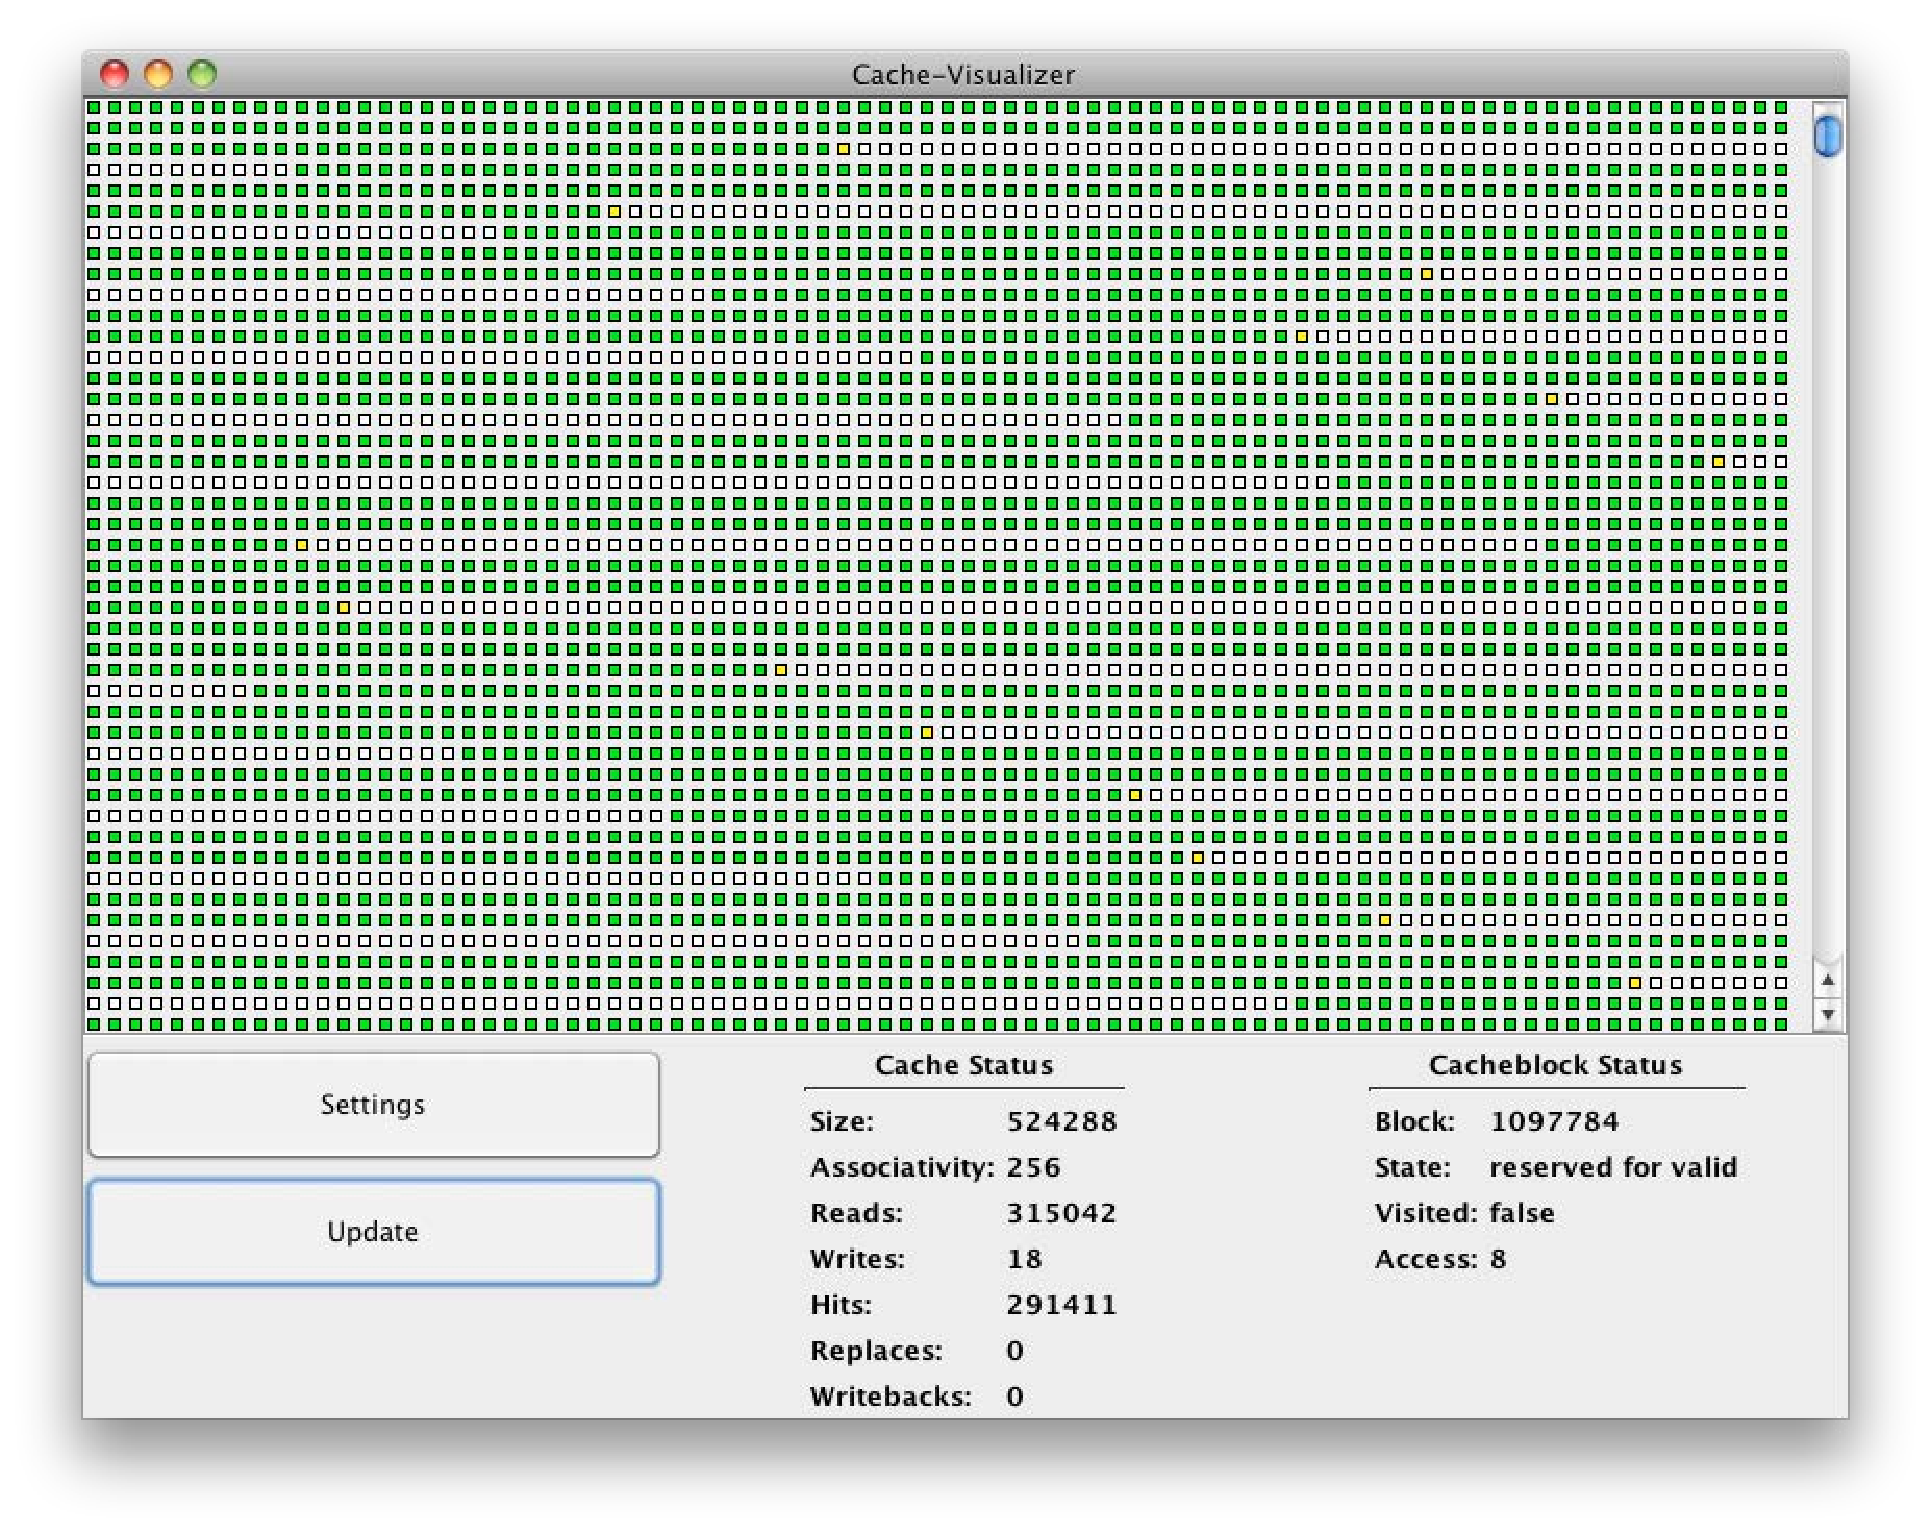
\includegraphics[scale=0.45]{figures/chapter6/screen}
    \caption[Fenster des Visualizers mit aktivem Cache]{Fenster des Visualizers mit aktivem Cache}
    \label{img:debug2}
\end{figure}
\vspace{5mm}
\section{Cache-Algorithmus}
\label{chap6:algo}

Für den in Abschnitt \ref{chap5:algo1} vorgestellten Verdrängungsalgorithmus mussten die Cacheblock-Metadatenstruktur zunächst um ein Feld für den Zähler
erweitert werden und die Cachemetadatenstruktur um einen Zähler je Set. Des Weiteren musste die Konstruktorroutine angepasst werden, so dass die Informationen
über die Werte $i$, $m$ und $s$ zur Laufzeit übergeben werden können. Außerdem wurde der Parameter für die Schreibstrategie erweitert, um das in Kapitel
\ref{chap5:algo1} beschriebene Verfahren zu unterstützen. Dies hat zur Folge, dass sich der Aufruf für das Erstellen eines Caches wie folgt erweitert:

\begin{flushleft}
\hspace{0.25cm} \small \texttt{echo [Startblock] [Endblock] cache [Quellgerät] [Cachegerät] 0 [Cacheblockgröße] [Cacheblöcke] [Assoziativität] [0|1|2]
\textbf{[s] [m] [i]} | dmsetup create [Name]}
\end{flushleft}

Weiterhin wurde die Art der Speicherung der Cacheblockzustände geändert. In der ursprünglichen Implementierung wurden Statusbits genutzt um einen Zustand zu
bestimmen. Dieses führte dazu, dass für das Speichern der Zustände mindestens\footnote{Es wurde in der konkreten Implementierung eine 16 Bit Variable benutzt.}
vier Bit benötigt wurden. Zudem machte es den Quelltext unübersichtlich, da auf den ersten Blick nicht zwingend klar war, in welchem Zustand ein Block beim
Setzen eines Bits gebracht wurde bzw. schon war. Dies ist gerade in Anbetracht der Synchronisation der beiden großen Programmteile kritisch. Aus diesem Grund
wurden die Statusinformationen auf eindeutige Zustände abgebildet und in eine leichter zu verstehende Zustandsmaschine überführt (Abbildungen \ref{img:fsm1} und
\ref{img:fsm2}). Für die bessere Verständlichkeit werden an dieser Stelle Write-Through- und Write-Back-Cache getrennt dargestellt. Die komplette
Zustandsmaschine des Caches findet sich im Anhang unter Abbildung \ref{img:fsm3}. Die Zustandsmaschine für den Write-Hybride-Cache entspricht der des
Write-Back-Caches, wobei der Zustand \texttt{Reserved for Dirty} und die Übergänge dorthin bzw. von dort abgehend entfallen.

\begin{figure}[H]\centering
	\subfigure[]{
		\includetikz[0.66]{figures/chapter6/fsm1}%
		\label{img:fsm1}
	}
	\hfill
	\subfigure[]{
		\includetikz[0.66]{figures/chapter6/fsm2}%
		\label{img:fsm2}
	}
	\caption[Zustände und Zustandsübergänge der Cacheblöcke]{Zustände und Zustandsübergänge der Cacheblöcke -- in (a) für die Write-Through-Konfiguration und in (b) für die Write-Back-Konfiguration}
\end{figure}

\section{Optimierung der Cacheblock-Metadaten}
\label{chap6:meta}

Um einen möglichst geringen Speicherverbrauch zu erreichen, mussten die Metadaten der Cacheblöcke optimiert werden. Diese enthielten in der ursprünglichen
Implementierung jeweils eine Liste, um die Anfragen aufzunehmen, die während der Bearbeitung eines Cacheblockes ankommen und nicht sofort bearbeitet werden
können. Da diese Listen von den beiden zueinander asynchron laufenden Programmteilen genutzt wurden, mussten die Zugriffe synchronisiert werden. Aus diesem Grund
gab es für jeden Cacheblock eine Schlossvariable. Dies bedeutete einen Speicherverbrauch von 38 Byte pro Cacheblock. Welche Auswirkung diese Größe auf den
Gesamtspeicherverbrauch des Caches hat wird in Abschnitt \ref{chap7:mem} ausführlich betrachtet.

Erste Tests ergaben jedoch, dass diese Listen relativ selten genutzt wurden. Aus diesem Grund wurden sie durch eine gemeinsame Liste pro Cacheblock ersetzt,
welche in den Gesamtcache-Metadaten untergebracht wurden. Dies benötigte mehrere Anpassungen im Quelltext. Zunächst wurde der Callback-Funktion für das
Zurückschreiben von Cache\-blö\-cken auf das Quellgerät lediglich eine Referenz auf den geschriebenen Cacheblock übergeben. Das war ausreichend, da der Cacheblock
alle Referenzen auf die zu verändernden Daten enthielt. Durch das Verschieben der Liste für ausstehende \ac{BIO}-Anfragen musste die übergebene Datenstruktur
angepasst werden, da diese Referenz nicht mehr in den Metadaten enthalten war. Hierfür wurden die Cacheblock-Metadaten in eine erweiterte Datenstruktur
verpackt, wie sie in Listing \ref{listing:cache2:adv_cacheblock} zu sehen ist.

\lstset{language=C,
		basicstyle=\ttfamily\scriptsize,
		backgroundcolor=\color{lightgray},
		captionpos=b, 
		tabsize=4,
		showstringspaces=false,
		keepspaces=true,
		linewidth=.85\textwidth,
		xleftmargin=.15\textwidth,
		commentstyle=\color{comment},
		keywordstyle=\bfseries\color{keyword},
		stringstyle=\color{string},
		morecomment=[s][\color{javadoc}]{/**}{*/}}

\lstinputlisting[frame=trbl,caption=Metadatenstruktur für die Übergabe an die Write-Back-Callback-Funktion, label=listing:cache2:adv_cacheblock]{listings/struct_adv_cacheblock.source}

Da es ineffizient wäre, alle \ac{BIO}-Aufträge lediglich hintereinander in eine Liste einzufügen und beim Callback des Kopiervorgangs die zu einem Cacheblock
gehörenden  \acp{BIO} herauszusuchen, sind die Einträge in der neuen Auftragsliste nach Cache\-blö\-cken sortiert. Aus dieser Anforderung ergab sich die
Listenform in Listing \ref{listing:cache2:queue}. Um nun nicht bei jedem Callback die Liste durchsuchen zu müssen, auch wenn keine ausstehenden Anfragen für einen
Cacheblock vorliegen, wurde ein zusätzliches Statusbit in die Cacheblock-Metadaten eingefügt. Dieses zeigt an, ob Aufträge für den Cacheblock vorliegen oder
nicht. Wenn dies nicht der Fall ist, braucht die Liste nicht durchsucht zu werden.

\lstinputlisting[frame=trbl,caption=Listenstruktur für ausstehende BIO-Aufträge, label=listing:cache2:queue]{listings/struct_queued_bios.source}

Durch die vorherigen Änderungen war es möglich, die Cacheblock-Metadatenstruktur im Hinblick auf den
Speicherverbrauch zu optimieren. Mit der bisher verwendeten 64-Bit langen Blocknummervariablen lassen sich bis zu $2^{64}$ Blöcke bzw. 16PB bei einer Blockgröße
von 512 Byte adressieren. Da diese Datenmenge in absehbarer Zeit nicht auf einem Gerät zur Verfügung stehen wird, wurden einige Bits dieser Statusvariablen für
die zusätzlichen Informationen verwendet. Die genaue Aufteilung der 64-Bit Variablen ist in Abbildung \ref{img:block} zu sehen. Die verbleibenden 56-Bit reichen
jedoch immer noch für 64EB Daten zu 512 Byte Blöcken. Da heutige Festplatten eine Kapazität von maximal 2TB aufweisen, ist es unwahrscheinlich, dass das Modul an
seine Grenzen stößt. Das Modul kann jedoch bei Bedarf auf größere Blocknummern umgestellt werden. So ist es in Zukunft möglich, größere Blockgeräte
zu unterstützen. Dabei dürfte auch der wachsende Speicherverbrauch unkritisch sein, da anzunehmen ist, dass die Größe des Arbeitsspeichers parallel zur
Festplattenkapazität wächst.

\begin{figure}[H]\centering
	  \includetikz{figures/chapter6/cacheblockmeta}%
    \caption[Aufbau der Cacheblock-Metadaten für das neue Kernelmodul]{Aufbau der Cacheblock-Metadaten für das neue Kernelmodul}
    \label{img:block}
\end{figure}

Die konkrete Implementierung der Datenstruktur (Listing \ref{listing:cache2:block}) zeigt, dass diese leicht erweiterbar ist. Der Zähler für den
Ersetzungsalgorithmus ist mit einer Länge von vier Bit an dieser Stelle sehr willkürlich gewählt und könnte auf Kosten der maximal addressierbaren Blöcke
problemlos erweitert werden, sollte sich dies zu einem späteren Zeitpunkt als Vorteilhaft erweisen.

\lstinputlisting[frame=trbl,caption=Optimiert Datenstruktur für Cacheblock-Metainformationen, label=listing:cache2:block]{listings/struct_cacheblock2.source}

\section{Anpassung der Metadatensicherung}
\label{chap6:save}

Auf Grund der Änderung der Cacheblock-Metadatenstruktur musste auch die Sicherung dieser Daten angepasst werden. Die Daten werden prinzipiell am Ende des
Cachegeräts gespeichert. Somit muss dieses nicht nur so groß sein wie der Cache, sondern um die Größe der Metadaten größer. Die ursprüngliche Implementierung
sorgte dafür, dass vor dem Speichern der Metadaten alle Cacheblöcke, die sich im \texttt{dirty} Zustand befanden, auf das Quellgerät zurückgeschrieben wurden.
Aus diesem Grund befanden sich beim Sichern alle Cachblöcke im \texttt{valid} oder \texttt{invalid} Zustand. Beim Sichern wurde lediglich der Status der
Cacheblöcke und die bei der Konstruktion übergebenen Parameter gesichert. Die logischen Zeitstempel wurden verworfen. Des Weiteren wurden die Informationen in
einem Puffer kopiert, da nur Datenblöcke mit einer Größe, die ein Vielfaches von 512 Byte sind, auf das Blockgerät geschrieben werden können.

Dieses Vorgehen wurde dahingehend geändert, dass nun sämtliche Metadaten der Cache\-blö\-cken gesichert werden.  Zusätzlich mussten im Gegensatz zu oben die Zeiger
für das Iterieren über den Sets gesichert werden. Es wird außerdem auf die Nutzung eines Puffers verzichtet, was das Schreiben und Wiederherstellen der Daten ein
wenig beschleunigt, da auf Kopiervorgänge im Speicher verzichtet werden kann. Dies bedeutet zwar ggf. einen Verschnitt, da der Speicherblock für die Metadaten
auf ein Vielfaches von 512 Byte aufgerundet werden muss. Da es jedoch nur zwei Speicherblöcke gibt (Cacheblock-Metadaten und Iterierungszeiger), kann der
Verschnitt nicht mehr als ein Kilobyte betragen.

Es wurde des Weiteren die Fehlererkennung bei der Wiederherstellung des Caches verbessert. Bei der ursprünglichen Implementierung wurden die gesicherten
Metadaten lediglich gelesen und wiederhergestellt. Dies führte dazu, dass bei einem Absturz des Systems und anschließendem Neustart die veralteten Metadaten
wiederhergestellt wurden. Dadurch kam es zu einem inkonsistenten Cache und im ungünstigsten Fall zum Datenverlust bzw. Absturz des Systems. Aus diesem Grund
wurde die Wiederherstellung verändert in der Weise, dass der ausgelesenen Cachemetadatenblock modifiziert wurde. Es ist ein Flag eingefügt worden, welches nach dem
Auslesen geändert und verändert zurück geschrieben wird. Dadurch war es möglich zu erkennen, ob die gelesenen Metadaten zu den auf dem Cachegerät gespeicherten
Datenblöcken passen. Sollte dies nicht der Fall gewesen sein, war es weiterhin dennoch möglich den Cache neu aufzubauen, sofern es sich um einen
Write-Through-Cache handelte. Bei einem Write-Back- bzw. Write-Hybrid-Cache kann auch durch dieses Verfahren der Cache nicht wiederhergestellt oder neu aufgebaut
werden, weil durch den Systemabstrurz die Metainformationen über die Cacheblöcke verloren gegangen sind und im Nachhinein nicht mehr festgestellt werden kann,
welche Cacheblöcke ausschließlich auf dem Cacheblockgerät aktuell sind und stattdessen auf dem Quellgerät gentutz werden müssten.

\section{\texttt{TRIM} Unterstützung}
\label{chap6:trim}

Das \texttt{TRIM}-Kommando wurde bereits in Kapitel \ref{chap2:ssd} erläutert. Es wurde ausgeführt, dass eine explizite Unterstützung in das Dateisystem
eingebaut werden muss. Bei der Implementierung des Caches war es jedoch möglich, für einen bestimmten Fall diese Unterstützung auch unabhängig vom Dateisystem
anzubieten. Wie in Abbildung \ref{img:fsm1} dargestellt, existiert beim Writh-Through-Cache ein Übergang in den \texttt{invalid} Zustand. An diesem Punkt ist die
Nutzung des \texttt{TRIM}-Kommandos sinnvoll, da der Inhalt des Cacheblockes nicht mehr benötigt wird und dies somit auch dem \ac{SSD} mitgeteilt werden kann.
Deshalb wird bei der Änderung des Cacheblock-Zustandes das \texttt{TRIM}-Kommando an das \ac{SSD} übermittelt. Dieses Verhalten ist zwar per Compiler-Makro ein-
und auschaltbar, jedoch sollte es selbst bei \acp{SSD} ohne \texttt{TRIM}-Unterstüztung zu keinem Leistungsverlust führen, da der Funktionsaufruf zum Löschen
asynchron ist (siehe \cite{linux:trim}) und sofort returnieren würde.

Das \texttt{TRIM}-Kommando fand jedoch auch Anwendung bei der Erstellung des Caches. Wie ebenfalls in Kapitel \ref{chap2:ssd} angesprochen wurde, nimmt die
Leistung eines \ac{SSD} über einen längeren Nutzungszeitraum ab, da zu wenige freie Blöcke zur Verfügung stehen. Dieses Szenario könnte vielleicht bereits beim
Nauaufbau eines Caches gegeben sein. Aus diesem Grund erschien es sinnvoll, vor der Nutzung den für den Cache vorgesehenen Datenbereich mit dem
\texttt{TRIM}-Kommando zu löschen. Dies ist nicht nur dahingehend sinnvoll, dass das \ac{SSD} bereits vor der Verwendung als Cache anderweitig genutzt wurde,
sondern auch für das Szenario, dass bei jedem Bootvorgang der Cache neu erstellt wird.

\section{Bootfähigkeit des Cachemediums}
\label{chap6:boot}

Das Booten eines Linuxsystems von einem Blockgerät setzt voraus, dass dieses beim Starten des \texttt{init}-Programms zur Verfügung steht. Da das
\texttt{dm-cache}-Modul in der ursprünglichen Implementierung eine Konfiguration aus dem Nutzerraum heraus erfordert, ist diese Voraussetzung nicht gegeben. Um
nun das Booten trotzdem zu ermöglichen gibt es zwei verschiedene Möglichkeiten. Die Erste nutzt das \textit{initramfs}. Da die Erklärung der genauen
Funktionsweise des \textit{initramfs'} den Rahmen dieser Arbeit sprengen würde, wird auf \cite{initramfs} verwiesen. Durch das \textit{initramfs} ist es möglich
zunächst ein gecachetes Blockgerät aus dem Nutzerraum zu erstellen und das Wurzeldateisystem drauf umzulenken.

Die zweite Möglichkeit besteht darin, die nötige Funktionalität für das Erstellen eines \ac{DM}-Blockgeräts direkt im Kernel fest zu implementieren, so dass beim
Übergang zum \texttt{init}-Programm das gecachte Blockgerät bereits existiert. Im offiziellen Entwicklungszweig des Linux-Kernels ist die Funktion zum Erstellen
von \ac{DM}-Geräte direkt aus dem Kernel heraus nicht vorgesehen. Es existiert jedoch bei \cite{boot-patch} ein Patch, der diese Funktion in den Kernel einfügt.
Durch diesen Patch ist es möglich, dem Kernel durch den Bootloader zusätzliche Parameter zu übergeben, um ein \ac{DM}-Gerät während des Bootens zu erzeugen. Der
zusätzliche Parameter sieht dabei wie folgt aus:

\begin{flushleft}
\hspace{0.25cm} \small \texttt{dm=\dq [name] [uuid] [ro], [parameter]\dq}
\end{flushleft}

Das \ac{DM}-Gerät wird zunächst unter dem Gerätepfad \texttt{/dev/dm-*} zur Verfügung gestellt. Hierbei steht das Sternchen für eine Nummerierung, welche bei bei
null beginnt. Dem Kernel muss somit das entsprechende Gerät im \texttt{root}-Parameter übergeben werden. Bei der Nutzung von \textit{udev} wird das Gerät beim
Booten zu \texttt{/dev/mapper/[name]} umbenannt, wobei \texttt{name} dem obigen im Kernelparameter entspricht. Weiterhin steht \texttt{uuid} für den \ac{UUID} ,
den das Gerät erhalten soll. Auf die Funktionsweise des \ac{UUID} soll in dieser Arbeit nicht genauer eingegangen werden, aber es wird hierfür auf \cite{uuid}
verwiesen. Soll dem Gerät kein \ac{UUID} zugewiesen werden, ist in das Feld \texttt{none} einzutragen. Der Parameter \texttt{ro} steht für die Einstellung, ob
vom \ac{DM}-Geräte lediglich gelesen oder sowohl gelesen als auch geschrieben werden kann. Die darauf folgenden Parameter entsprechen im wesentlichen den an
\texttt{dmsetup} übergebenen Parametern zum Erstellen eines \ac{DM}-Geräts. Somit würde der Kernelparameter für ein gecachetes Blockgerät, welches unter
\texttt{/dev/mapper/cached} zur Verfügung gestellt wird, wie folgt aussehen:

\begin{flushleft}
\hspace{0.25cm} \small \texttt{dm=\dq cached none 0, [Startblock] [Endblock] cache [Quellgerät] [Cachegerät] 0 [Cacheblockgröße] [Cacheblöcke] [Assoziativität]
[0|1|2] [s] [m] [i]\dq}
\end{flushleft}

Dabei wird ein neuer Cache erstellt. Um einen bestehenden Cache wiederherzustellen, muss der Kernel-Parameter wie folgt lauten:

\begin{flushleft}
\hspace{0.25cm} \small \texttt{dm=\dq cached none 0, [Startblock] [Endblock] cache [Quellgerät] [Cachegerät] 1\dq}
\end{flushleft}

Mit dem bestehenden Patch funktionierte das Erstellen des gecachten Mediums und Booten an sich problemlos. Der Patch hatte jedoch das Defizit, dass die
Destruktionsroutine des Caches beim Herunterfahren des Systems nicht aufgerufen wurde. Ebenfalls war es nicht möglich die Destruktionsroutine aus dem Nutzerraum
während des Herunterfahrens aufzurufen, da das gecachte Gerät als Rootdateisystem eingebunden war. Dies zog einen Verlust der Metadaten nach sich und verhinderte
das erneute Booten. Somit war der Cache in diesem Zustand als Rootdateisystem nicht nutzbar. Es musste ein Weg gefunden werden, durch den beim Herunterfahren
bzw. Neustart des Systems die Metadaten gesichert werden können. Hierbei gab es wiederum zwei Möglichkeiten. Zum einen eine Erweiterung des \ac{DM}-Frameworks
und zum anderen die Erweiterung des Cachemoduls. Auf Grund der beschränkten Bearbeitungszeit wurde auf die allgemeinere Implementierung im \ac{DM} verzichtet
und statt dessen das Cachemodul entsprechend erweitert.

Zunächst musste das Cachemodul in der Art erweitert werden, dass es über das bevorstehende Herunterfahren informiert wird. Hierfür wurden Linux
\textit{Notifiers} (siehe \cite{notifiers}) genutzt. Diese ermöglichen es, im Kernel einen Funktionsaufruf zu registrieren, welcher beim Herunterfahren bzw.
Neustart des Systems ausgeführt wird. Die hierbei übergebene Funktion wurde in der Art gestaltet, dass sie über alle verbliebenen Caches iteriert und
jeweils die Destrukturfunktion aufruft. Die Erweiterung ist in Listing \ref{listing:reboot} zu sehen.

Wie in den Zeilen 7ff zu erkennen ist, bedurfte es einer Liste aller verbleibenden Caches. Hierfür musste das Kernelmodul wiederum erweitert werden, da das
\ac{DM}-Framework keine Funktionalität vorsieht, welche das Abfragen nach \ac{DM}-Geräten eines bestimmten Typs ermöglicht. Aus diesem Grund wurde die
Cachemetadatenstruktur zu einer Kernel-Liste erweitert (vgl. Zeile 7 Listing \ref{listing:cache2:meta} im Anhang). Vom Modul selbst wird nun eine Liste aller
Cachemetadatenstrukturen verwaltet. Hierbei wird beim Erstellen eines Caches die entsprechende Struktur zur Liste hinzugefügt und beim Entfernen des Caches die
Struktur ebenfalls aus der Liste entfernt. Mit dieser Liste ist es nun möglich, bei der Benachrichtigung über das Herunterfahren die Metadaten aller Caches zu
sichern.

\lstset{language=C,
		basicstyle=\ttfamily\scriptsize,
		backgroundcolor=\color{lightgray},
		captionpos=b, 
		tabsize=4,
		showstringspaces=false,
		keepspaces=true,
		linewidth=.95\textwidth,
		xleftmargin=.05\textwidth,
		commentstyle=\color{comment},
		keywordstyle=\bfseries\color{keyword},
		stringstyle=\color{string},
		morecomment=[s][\color{javadoc}]{/**}{*/}}
\lstinputlisting[frame=trbl,caption=Erweiterung für das automatische Entfernen des Caches beim Herunterfahren,label=listing:reboot]{listings/reboot.source}
 \cleardoublepage{}
\chapter{Auswertung}
\label{chap7}

Nachdem in den beiden vorangegangenen Kapiteln die Architektur und die Implementierung des entwickelten Kernelmoduls thematisiert wurden, sollen nun die damit
erzielten Ergebnisse diskutiert werden. Dabei wird zunächst in Abschnitt \ref{chap7:synth} ein synthetisches Testszenario betrachtet. Im darauf folgenden
Abschnitt \ref{chap7:boot} wird ein reales Szenario ausgewertet. Abchließend wird in Abschnitt \ref{chap7:mem} sowohl die Rechenlast als auch der
Speicherverbrauch des Moduls untersucht und diskutiert. Für die Tests wurden, sofern nicht anders angegeben, als Festplatte eine Western Digital Raptor
mit 73,4GB Kapazität~\cite{wd:raptor} und als SSD eine Intel X25-E mit 32GB Kapazität~\cite{intel:ssd} genutzt.

\section{Synthetische Leistungsbewertung}
\label{chap7:synth}

Die Leistung des implementierten Kernelmoduls wird in diesem Kapitel anhand eines eigens entworfenen Testszenarios ermittelt. Hierfür wird im ersten
Unterabschnitt zunächst das Testszenario genauer beschrieben. Anschließend werden in Unterabschnitt \ref{chap7:synth:results} die mit Hilfe des Szenarios
gewonnen Testergebnisse vorgestellt und diese abschließend in Unterabschnitt \ref{chap7:synth:discu} diskutiert.

\subsection{Testszenario}
\label{chap7:synth:szenario}

Das synthetische Testszenario, das im Rahmen dieser Arbeit entwickelt wurde, musste zunächst die Hauptanforderung der Vergleichbarkeit der Systemkonfigurationen
erfüllen. Hierfür mussten die Simulationen wiederholbar sein. Neben dieser Hauptanforderung musste es zusätzlich verschiedene Nebenanforderungen erfüllen. Die
Erste besteht darin, die besonderen Eigenschaften eines Caches überhaupt nutzen zu können. Ein gecachtes Medium kann gegenüber einem ungecachten Medium
prinzipbedingt nur einen Geschwindigkeitsvorteil realisieren, wenn auf dieselben Daten mehrfach zugegriffen werden kann. Aus diesem Grund sind die meisten
gebräuchlichen Festplattenbenchmarks bereits ungeeignet. Des Weiteren stellen diese Benchmarks meist ein synthetisches Testszenario dar, welches ebenfalls für
diese Arbeit nicht gewünscht war.

Neben den genannten synthetischen Benchmarks wurde eine andere Möglichkeit in den Arbeiten genutzt, die in Kapitel \ref{chap3} vorgestellt wurde und
vergleichbare Szenarien benötigt. Diese besteht darin, zunächst die Anfragen eines realen Systems an ein Blockgerät aufzuzeichnen. Für den eigentlichen
Benchmark können anschließend die Anfragen an die zu testenden Geräte gestellt und die Verarbeitungszeiten verglichen werden. Dieses Testszenario hat jedoch den
Nachteil, sehr zeitintensiv zu sein, denn zunächst müssen die Daten auf einem Produktivsystem gesammelt werden. Um einen repräsentativen Datensatz zu erhalten
müsste dies über mehrere Tage oder gar Wochen geschehen. Anschließend wären vergleichbare zeitliche Dimensionen nötig, um einen Testlauf durchzuführen. Da im Rahmen
dieser Arbeit mehrere Konfigurationen getestet werden sollten, könnte sich der Zeitbedarf leicht auf Monate summieren. Außerdem würde der Aufbau der nötigen
Infrastruktur zur Aufzeichnung von Datensätzen mit einem nicht vernachlässigbaren Aufwand verbunden sein. Aus diesem Grund konnte dieses Testszenario für diese
Arbeit ebenfalls nicht verwendet werden.

Aus den genannten Gründen ist als Kompromiss ein Zwischenweg aus den beiden genannten Möglichkeiten gewählt worden. Es wurde der synthetische
Benchmark \textit{\mbox{bonnie++}}~\cite{bonnie} hierfür angepasst. \textit{\mbox{Bonnie++}} ist ein synthetischer, auf Dateisystemebene arbeitender, nicht
destruktiver\footnote{Bereits bestehende Daten auf dem Datenträger bleiben erhalten.} Benchmark, welcher Daten auf das zu testende Gerät schreibt und geordnet
und ungeordnet ausliest. Dabei werden die benötigte Zeit und die Prozessorlast gemessen. Da jedoch bei jedem Testlauf die Dateien neu generiert werden mußten,
konnten mit der ursprünglichen Implementierung die Eigenschaften eines Caches nicht genutzt werden. Aus diesem Grund wurde das Programm im Rahmen dieser Arbeit
erweitert, so dass es eine Dateiliste einlesen kann und Lese-/Schreibvorgänge entsprechend dieser Liste durchführt. Dabei besteht die Dateiliste aus mehrere
Zeilen, die wie folgt aufgebaut sind:

\begin{flushleft}
\hspace{0.25cm} \small \texttt{[Dateiname], [Dateigröße], [c|s|d]}
\end{flushleft}

Beim Ausführen von  \textit{\mbox{bonnie++}} wird die Liste eingelesen und je nach dem letzten Parameter die Datei mit der gegebenen Größe erstellt (c), gelesen (s)
oder gelöscht (d). Mit Hilfe dieser Modifikation ließ sich nun ein realitätsnahes Testszenario aufbauen. Um ein reales Desktopsystem zu simulieren, musste
zunächst die Installation und der Bootvorgang simuliert werden. Hierfür wurde als erstes die Datei- und Verzeichnisstruktur eines Ubuntu-Linux-Systems extrahiert
und eine Dateiliste mit dem oben gezeigten Format erstellt, die ihrerseits für das Erstellen von Dateien sorgt. So kann die Installation des Systems simuliert
werden. Die Liste beinhaltet hierbei knapp 121000 Dateien mit einer Gesamtgröße von ca. 3,6GB. Als zweiter Schritt wurde die Menge der gelesen Daten beim Booten
des realen Linux-Systems gemessen. Diese lag bei ca. 150MB. Anschließend wurden aus der Dateiliste des Linux-Systems zufällige Dateien gewählt, die eine
Gesamtgröße von 150MB hatten, und damit eine \textit{\mbox{bonnie++}} Dateiliste erstellt, die das Lesen dieser Dateien durch \textit{\mbox{bonnie++}} veranlasst. Diese
Dateiliste wurde einmalig erstellt und während der Tests nicht verändert. Mit der Liste ließ sich das Booten des Systems und das Starten der Programme annähernd
genau simulieren.

Abschließend musste eine Möglichkeit gefunden werden, das Erstellen, Lesen und Löschen von Nutzerdaten zu simulieren. Hierfür wurden Datenlisten erstellt, die
Angaben zu Dateien mit einer Gesamtgröße von 100MB enthielten. In den Listen überwog dabei die Anzahl von kleinen Dateien stark. Diese Listen wurden
ebenfalls einmalig erzeugt und während der Tests nicht mehr verändert. Bei der Simulation wurden nach jedem simulierten Bootvorgang eine gewisse Anzahl $r$
dieser Sets gelesen, $c\,$ Sets geschrieben und $d$ wieder gelöscht. Dabei wurde die Reihenfolge, welche Sets gelesen, geschrieben oder gelöscht werden,
einmalig festgelegt und ebenfalls während aller Tests nicht verändert. Dieses Vorgehen sollte nun zusammen mit dem Bootvorgang einen Arbeitstag simulieren.

Ausnahmen von dem soeben beschriebenen Vorgehen bildeten die ersten Bootvorgänge einer jeden Simulation. Hierbei wurden jeweils doppelt so viele Sets wie
gewöhnlich geschrieben, bis eine Maximalanzahl $M$ von Sets auf der Festplatte vorhanden waren. Beim Lesen wurden alle Sets berücksichtigt, solange die Anzahl
von Sets auf den Datenträgern den Wert $r$ nicht überstiegen. Des Weiteren wurde beim Erstellen der Erstellungs-, Lese- und Löschreihenfolge der Sets darauf
geachtet, dass immer ein Set existierte, welches an jedem Arbeitstag gelesen wurde. Dieses sollte regelmäßig genutzte Daten simulieren. Die Reihenfolge der
Arbeitstage wurde ebenfalls im Vornherein festgelegt und während der verschiedenen Simulationsläufe nicht verändert. Somit soll an dieser Stelle noch einmal
betont werden, dass alle zufälligen Festlegungen vor dem Beginn der Evaluierung stattfanden.

Bei den konkreten Tests auf einem System galt es jedoch noch eine weitere Funktion des Linux-Systems zu beachten -- nämlich den Datencache im Arbeitsspeicher.
Dieser verzerrte die Messergebnisse des Benchmarkprogramms, da das Betriebssystem den Abschluss von Dateioperationen meldet, obwohl diese noch nicht auf dem
Blockgerät abgeschlossen sind. Weiterhin konnten durch den Arbeitsspeichercache Daten von mehreren Arbeitstagen gehalten werden, so dass z.B. die Daten des Bootens
nicht zwingend vom Blockgerät gelesen wurden sondern aus dem Arbeitsspeichercache. Erste Tests zeigten, dass die Verzerrungen durch diesen Mechanismus enorm
waren und ein Vergleich der verschiedenen zu testenden Konfigurationen nicht möglich war. Zwar war es möglich, die Funktion abzuschalten, was jedoch
zu erheblichen Leistungsverlusten führte, die die Messungen wiederum unrealistisch machten. Das Problem der Übertragung von Daten von einem Bootvorgang zum
Nächsten durch den Arbeitsspeichercache ließ sich durch das Neueinhängen des Blockgerätes in das Dateisystem lösen, da dies das Linux-System dazu veranlasste den
Arbeitsspeichercache zu leeren. Jedoch waren die von \textit{\mbox{bonnie++}} gelieferten Messwerte bezüglich der Leserate ungenau. Um dies Problem zu lösen, wurde als
Maßstab für die Leistung die Zeit zwischen Ein- und Aushängen des Blockgerätes genutzt.

\subsection{Ergebnisse}
\label{chap7:synth:results}

Beim Erstellen einer konkreten Testumgebung sind weitere Dinge zu beachten. Zum einen sollte die gelesene Datenmenge größer sein als der Cache. Ist dies nicht
der Fall, können sämtliche Daten im Cache gehalten werden und es sind keine Rückschlüsse auf die Effizienz des Verdrängungalgorithmuses möglich. Zum anderen ist
die Laufzeit des Tests zu beachten. Wenn von einem momentan üblichen \ac{SSD} und somit auch einer Cachegröße von 32GB ausgegangen wird, würde dies bedeuten,
dass pro simuliertem Arbeitstag mehr als diese 32GB gelesen werden sollten. Das würde zunächst im optimalen Fall bei einer Leserate von 250MB/s und 50
simulierten Arbeitstagen eine Testlaufzeit von ca. zwei Stunden bedeuten. Weiterhin bietet der implementierte Cache sehr viele Freiheitsgrade. Das sind die
Assoziativität, die Cacheblockgröße und die Cacheparameter $m$, $s$ und $i$. Beides in Kombination würde Simulationszeiten von mehreren Monaten bedeuten, sofern
sämtliche Konfigurationskombinationen getestet werden sollten. Dies war im Zeitrahmen dieser Arbeit jedoch nicht möglich. Aus diesem Grund mussten sowohl
Einschränkungen bei der Testumgebung hingenommen werden als auch bei der Anzahl der durchgeführten Simulationen.

Zunächst wurde die Größe des Caches künstlich auf zwei Gigabyte beschränkt. Weiterhin wurde darauf verzichtet, an jedem simulierten Arbeitstag mehr Daten zu
lesen, als der Cache halten kann. Durch eine ausreichend große Anzahl an verschiedenen Datensets auf dem Quellmedium und das Löschen und Schreiben von Sets wurde
jedoch sichergestellt, dass die Datenmenge über mehrere simulierte Tage verteilt größer ist als der Cache. Konkret bedeutet dies Werte von $M=20$, $r=9$, $c=1$
und $d=1$.

Außerdem musste bei den Cacheparametern stark selektiert werden. Dies war notwendig, da die Simulationszeiten starken Schwankungen unterlagen. Beim Erstellen
der Vergleichswerte von der genutzten Festplatte und dem \ac{SSD} kam es zu Abweichungen von bis zu 7,3\% bzw. 9,8\% vom Mittelwert bei Festplatte bzw.
\ac{SSD}. Dies bedeutete, dass jede Konfiguration mehrfach getestet werden musste, um Ausreißer zu vermeiden. Daher wurde zunächst die Blockgröße auf vier
Kilobyte festgelegt. Dies ist die kleinstmögliche sinnvolle Größe, da sie der Blockgröße des verwendeten \ac{ext3} entspricht. Weiterhin wurde der Cacheparameter $m$ auf die Werte $\{4;8;16\}$
beschränkt und die Werte $i$ und $s$ auf $\{1;m\}$. Der Wert von $i=1$ bringt hierbei den Cache näher an einen LFU-Cache und der Wert $i=m$ näher an einen
LRU-Cache. In Abbildung \ref{img:time16} sind die Ergebnisse für $m=16$ dargestellt, wobei für die Assoziativität die Werte
$\{2;4;8;16;32;128;512;2048;8192;32768;131072\}$ genutzt wurden. Für die Werte $m=4$ und $m=8$ konnte die Simulation nur einmal durchgeführt werden, wodurch die
Ergebnisse sehr mit Ausreißern behaftet sind. Aus diesem Grund finden sie sich im Anhang unter \ref{img:time4} und \ref{img:time8}. Wie aus den Diagrammen 
ersichtilich ist, war es lediglich möglich ein spezifisches \ac{SSD} zu nutzen, da sich ansonsten der Testaufwand wiederum verdoppelt hätte.

\begin{figure}[b!]\centering
    \includetikz{figures/chapter7/time16}%
    \caption{Benchmarkergebnisse des Caches für $m=16$}
    \label{img:time16}
\end{figure}

Die Tests konzentrierten sich im weiteren Versuchsaufbau auf die Write-Through-Kon\-fi\-gu\-ra\-tion. Dies liegt zum einen darin begründet, dass die beiden anderen
Konfigurationen nicht im Zeitrahmen dieser Arbeit stabil implementiert werden konnten. So kam es zu sporadischen Synchronisationsproblemen, welche zukünftig noch genauer
analysiert werden müssen. Zum anderen konnten bei stichprobenartigen Tests der Write-Hybrid-Strategie nur unwesentliche Leistungsunterschiede zur
Write-Through-Strategie festgestellt werden. Die Write-Through Strategie lieferte bei der Simulation sehr schlechte Ergebnisse. Die Laufzeit der Simulationen lag
bei allen getesteten Konfigurationen um mehr als das Doppelte über denen der Festplatte. Die genauen Ursachen hierfür werden im Diskussionsteil näher ergründet.

Neben dem Vergleich mit den ungecachten Medien sollte der implementierte Cache zusätzlich mit dem von ZFS verglichen werden. Hierfür wurde die Testumgebung
zunächst für OpenSolaris portiert, da für Linux keine ausgereifte ZFS Implementierung existiert. Anschließend wurden erneut Messwerte für Festplatte und
\ac{SSD} ermittelt, da ein anderes Dateisystem neben der Nutzung eines Caches auch hier eine andere Leistung aufweisen könnte. Wie jedoch in Abbildung \ref{img:time-zfs}
zu sehen ist, war dies nicht der Fall. Anschließend wurde der Test für einen durch das \ac{SSD} gecachten Pool wiederholt. Dieses Ergebnis findet sich ebenfalls
in Abbildung \ref{img:time-zfs} mit dem Messwert für eine Assoziativität von 2048 aus der obigen Messung.

\begin{figure}[b!]\centering
    \includetikz{figures/chapter7/zfs}%
    \caption{Vergleich zwischen dem implementierten Cache und ZFS}
    \label{img:time-zfs}
\end{figure}

Die oben beschriebenen Messungen wurden mit dem sehr performanten Intel-\ac{SSD} durchgeführt. Bei der Simulation mit einem midrange \ac{SSD} (OCZ Vertex Series
32GB~\cite{ocz:ssd}) kam es zu massiven Leistungseinbrüchen. Die Ursache hierfür war in der Größe der Cache\-block\-größe zu finden, welche ungünstig für das
spezifische \ac{SSD} war. Das Diagramm in Abbildung \ref{img:size} zeigt die Leistung des midrange \ac{SSD} in Abhängigkeit von der genutzten Cacheblockgröße.
Die Gründe für die Leistungsunterschiede sollen im nun folgenden Unterabschnitt \ref{chap7:synth:discu} diskutiert werden.

Es konnten im Rahmen dieser Arbeit keine fundierten Messwerte ermittelt werden be\-züg\-lich des Nutzens des \texttt{TRIM}-Kommandos. Dies lag daran, dass lediglich
ein \ac{SSD} zur Verfügung stand, die diese Funktion unterstützt. Bedauerlicherweise konnten mit ihr jedoch keine verwertbaren Messwerte bezüglich der
Cache-Leistung gewonnen werden, so dass auch kein Vergleich zwischen ein- und ausgeschalteter \texttt{TRIM}-Unterstützung ermittelt werden konnte.

\begin{figure}[b!]\centering
    \includetikz{figures/chapter7/size}%
    \caption[Benchmarkergebnisse des Caches für verschiedene Cacheblockgrößen]{Benchmarkergebnisse des Caches für verschiedene Cacheblockgrößen ($m=16$, $s=1$,
    $i=1$)}
    \label{img:size}
\end{figure}

\subsection{Diskussion}
\label{chap7:synth:discu}

Die Ursachen für die Leistungsunterschiede, die im vorangegangenen Abschnitt aufgezeigt wurden, lassen sich über die
verschiedenen internen Blockgrößen und Controller der \acp{SSD} erklären. Abbildung \ref{img:cb} zeigt die Leistung verschiedener \acp{SSD} in Abhängigkeit von
der angeforderten Blockgröße. Es ist klar zu erkennen, dass die Leistung des \ac{SSD}s unter einer individuellen Blockgröße stark sinkt. Dies bedeutet, dass
bei der Wahl der Cacheblockgröße dieser Sachverhalt zu beachten ist. Allerdings kann die Cacheblockgröße nicht ohne weiteres an die native Blockgröße des
jeweiligen \ac{SSD}s angepasst werden. Die Vergrößerung der Cacheblockgröße über das der Dateisystemblockgröße hinaus hat den Nachteil, dass ggf. Daten im Cache
liegen, die nicht benötigt werden. Sollte die Cacheblockgröße z.B. 256kB betragen und eine Datei von vier Kilobyte oft genutzt werden, würde zunächst für diese
Datei ein 256kB Block im Cache eingelagert werden. Im ungünstigsten Fall werden die restlichen 252kB Daten extrem selten bis gar nicht genutzt. Dies könnte z.B.
bei Sicherungskopien der Fall sein. Also würden über 98\% der Daten in diesem Block unnötig vorgehalten werden. Wenn dieses Verhältnis auf den Rest des
Caches übertragen wird, würde im Realfall dieser Wert bei weitem nicht erreicht werden, da es extrem unwahrscheinlich ist, dass die Daten auf dem Quellmedium
entsprechend ungünstig verteilt sind. Es ist jedoch möglich, dass ein nicht unerheblicher Teil des Platzes im Cache blockiert wird, was zu Leistungseinbußen
führt. Dies ist bei der Leistungskurve des zwei Gigabyte Caches zu beobachten. Darum sollte die individuelle Größe der Cacheblockgröße insbesondere bei kleinen
Cachegeräten durch Benchmarks ermittelt werden.

\begin{figure}[b!]\centering
    \includetikz{figures/chapter7/cb}%
    \caption[Datendurchsatz verschiedener SSDs]{Datendurchsatz verschiedener SSDs in Kilobyte pro Sekunde in Abhängigkeit der Blockgröße (Quelle: \textcite{cb} und Eigenmessungen)}
    \label{img:cb}
\end{figure}

Wie in Abbildung \ref{img:time16} zu erkennen ist, hängt die Leistung des Caches bei gleicher Größe in erster Linie von der Assoziativität ab. Es ist mit
Ausnahme der Konfiguration $m=16$, $s=1$, $i=16$ sichtbar, dass die Leistung des Systems mit zunehmender Assoziativität steigt. Dieses Verhalten war zu erwarten,
da bei einer niedrigen Assoziativität die Wahrscheinlichkeit einer Kollision steigt. Bei der Betrachtung des Extremfalls mit einer Assoziativität von eins würden
alle Festplattenblöcke, die voneinander einen Abstand haben, der der Cachegröße entspricht, in den selben Cacheblock fallen. Die Wahrscheinlichkeit, dass dies
passiert, ist sehr hoch und führt zu Leistungseinbußen, da ggf. leere Teile des Caches nicht genutzt werden können. Wenn nun die Assoziativität erhöht wird,
können kollidierende Blöcke eher in einen leeren Bereich des Caches eingelagert werden. Dies ist bei dem anderen Extrem der Fall, bei dem die Assoziativität
genauso groß ist wie der Cache, d.h. der Cache nur aus einem Set besteht. Hierbei kommt es erst zu Verdrängungen, wenn der Cache komplett gefüllt ist. Wie in
Abbildung \ref{img:time16} zu erkennen ist, sinkt die Leistung des Caches ab einem bestimmten Assoziativitätsgrad wieder. Die Ursache hierfür ist die Größe der
Sets. Je größer ein Set ist, umso größer ist der Aufwand, einen Block zu finden, der potentiell in diesem Set liegt. Somit lässt sich ein Tradeoff zwischen
ineffizienter Verdrängung und Rechenleistung feststellten.

Das Abweichen der Konfiguration $s=1$ und $i=16$, lässt sich nicht ohne weiteres erklären, insbesondere da die Simulationen mit $m=4$ und $m=8$ diese Anomalie
bei vergleichbaren Werten für $s$ und $i$ nicht aufweisen. Ganz im Gegenteil, sie zeigen eine ähnliche Anomalie jedoch für andere $s$- und $i$-Werte. Es müsste
zunächst durch längere Simulationen ermittelt werden, ob es sich bei den Messwerten lediglich um statistische Ausreißer handelt oder ob die Ergebnisse
representativ sind. Sollte dies der Fall sein, ist es nötig, dass die genauen Ursachen detailliert untersucht werden. Des Weiteren ist festzustellen, dass
abgesehen von den Anomalien die Manipulation der Werte $s$ und $i$ keine signifikanten Unterschiede liefern. Die Wirkung der Änderung des Wertes $m$ kann nicht
genau bestimmt werden, da die Messwerte bei einer zu hohen Varianz zu dicht beieinander liegen.

Ferner wurde oben festgestellt, dass die Write-Back-Konfiguration eine sehr schlechte Leistung liefert. Die Ursache hierfür ist im Aufbau des Tests zu suchen;
genauer gesagt beim Schreiben neuer Daten. Diese werden sequenziell auf den Datenträger geschrieben, was sowohl bei der Festplatte als auch bei dem \ac{SSD} sehr
schnell vor sich geht. Durch den Write-Back-Cache werden diese sequenziellen Schreibvorgänge jedoch in ungeordnete transformiert. Dies geschieht dadurch, dass
ein Teil des sequenziellen Datenstroms auf das Cachegerät geschrieben wird und der andere Teil direkt auf das Quellgerät. Dies teilt den sequenziellen Datenstrom
zunächst in zwei ungeordnete Datenströme auf, was direkt zu massiven Leistungseinbußen führt, da die Festplatten beim ungeordneten Schreiben signifikant
langsamer werden als beim geordneten. Auch beim \ac{SSD} ist ein ähnliches Verhalten zu beobachten, wenn auch bei weitem nicht im selben Ausmaß. Das Problem wird
jedoch sogar weiter intensiviert, da die Wahrscheinlichkeit groß ist, dass die auf dem Cachegerät eingelagerten Daten zu einem späteren Zeitpunkt wieder auf das
Quellgerät zurückgeschrieben werden müssen. Auch dies geschieht wieder ungeordnet, so dass der ursprünglich gesamte sequenzielle Datenstrom als ungeordneter
Datenstrom auf die Festplatte geschrieben wird.

Abschließend gilt es noch, die Leistung des blockbasierten Caches gegenüber dem Cache des ZFS-Dateisystems zu beurteilen. Es ist in Abbildung \ref{img:time-zfs}
ganz klar und deutlich erkennbar, dass bei guter Wahl der Cacheparameter der blockbasierte Cache dem von ZFS in nichts nachsteht. Ganz im Gegenteil, er kann
sogar einen kleinen Leistungsvorsprung für sich verbuchen. So kann an dieser Stelle festgehalten werden, dass ein blockbasierter Cache gegenüber einem
Dateisystem basierten Cache konkurrenzfähig ist. In Anbetracht dessen, dass der blockbasierte Cache universeller einsetzbar ist, sollte die Nutzung dessen weiter
erforscht werden.

\section{Reale Leistungsbewertung}
\label{chap7:boot}

Nachdem im vorangegangenen Abschnitt die Leistung unter einem synthetischen Test betrachtet wurde, soll in diesem Abschnitt die Leistung unter einem realen Test
bewertet werden. Erneut wird im ersten Unterabschnitt das Testszenario beschrieben, im Zweiten die Ergebnisse dargestellt und im Dritten die Ergebnisse
diskutiert.

\subsection{Testszenario}

Als Testszenario dient der Bootvorgang eines Linux Systems. Dafür wurde die Gentoo-Distribution gewählt, da sich mit ihr der Startvorgang sehr einfach
benutzerspezifisch anpassen lässt. Andere Distributionen, wie z.B. die im vorherigen Kapitel simulierte Ubuntu-Distribution, sind auf Benutzerfreundlichkeit und
einfache Wartung ausgelegt. Hierbei ist eine Anpassung des Bootvorgangs relativ kompliziert, da von den Entwicklern eine weitreichende Nutzeranpassung des
selbigen nicht vorgesehen ist. Bei der Gentoo-Distribution ist dies nicht der Fall, weil sie sich hauptsächlich an Experten wendet und jedes Details des
Bootvorgangs einfach kontrollier- und anpassbar ist.

Für die Leistungsmessung wurde zunächst ein Standardsystem mit Gnome-Desktop installiert. Zur detaillierten Bewertung des Bootvorgangs wurde weiterhin das
Evaluierungsprogramm \textit{Bootchart} \cite{bootchart} installiert. Dieses misst die Zeit zwischen dem Start des \texttt{init}-Programms und des
Login-Bildschirms des Gnome-Desktops. Weiterhin werden Informationen über die Prozessorauslastung, Ein-/Ausgabewartezeiten, Datendurchsatz der Plattengeräte und
deren Auslastung gelogt. Ferner werden die gestarteten Prozesse in Abhängigkeit voneinander dargestellt. Somit ist es möglich den Bootvorgang zu analysieren
und ggf. Leistungsengpässe zu bestimmen.

\subsection{Ergebnisse}

\begin{figure}[b!]
    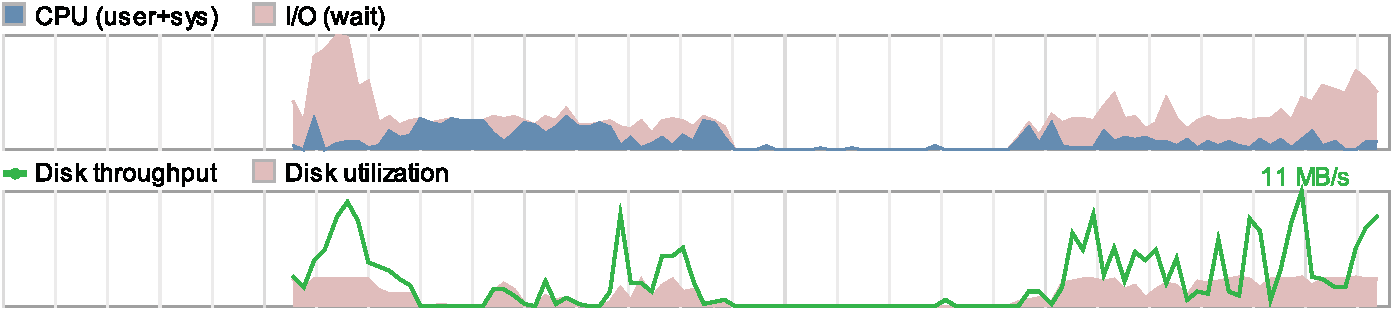
\includegraphics[scale=0.543]{figures/chapter7/boot-hdd}%
    \caption{Leistungsdaten eines HDD-Bootvorgangs}
    \label{img:boot:hdd}
\end{figure}

\begin{figure}[b!]
    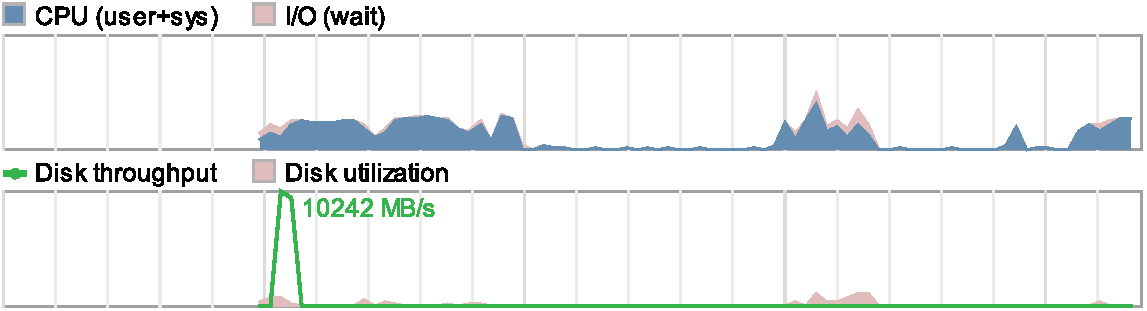
\includegraphics[scale=0.543]{figures/chapter7/boot-ssd}%
    \caption{Leistungsdaten eines SSD-Bootvorgangs}
    \label{img:boot:ssd}
\end{figure}

\begin{figure}[b!]
    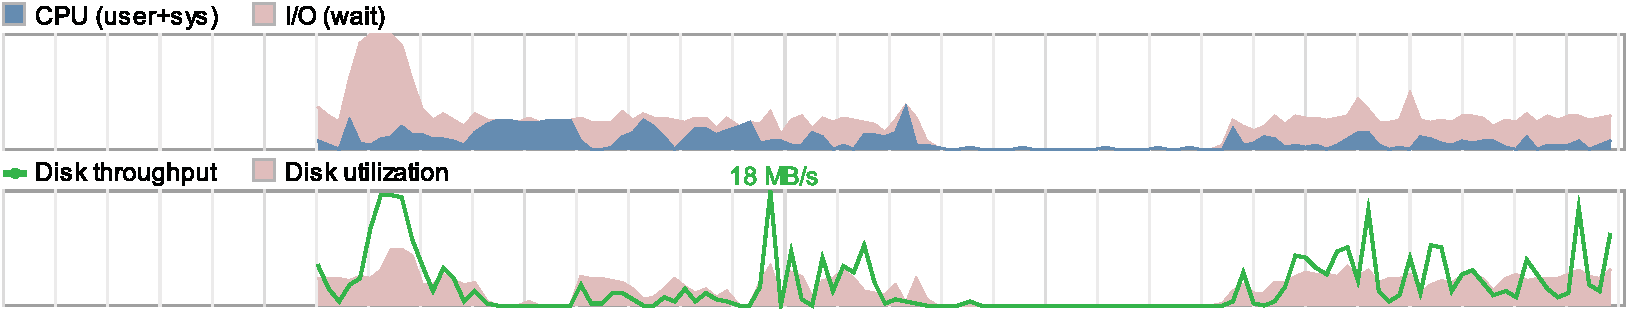
\includegraphics[scale=0.543]{figures/chapter7/boot-cache1}%
    \caption{Leistungsdaten des ersten Cache-Bootvorgangs}
    \label{img:boot:cache1}
\end{figure}

\begin{figure}[b!]
    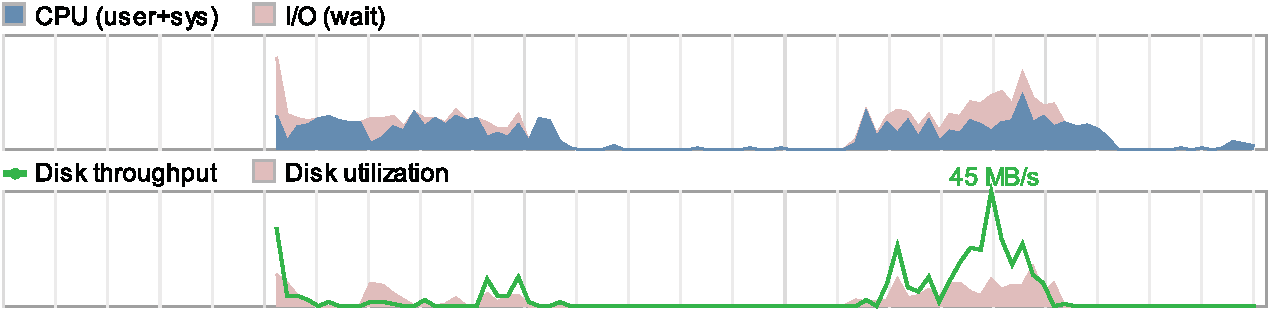
\includegraphics[scale=0.543]{figures/chapter7/boot-cache2}%
    \caption{Leistungsdaten des zweiten Cache-Bootvorgangs}
    \label{img:boot:cache2}
\end{figure}

Die Analyse der Bootvorgänge erfolgte für vier konkrete Szenarien. Es wurde die im letzten Abschnitt erwähnte Western Digital Raptor als Festplatte
und als \acp{SSD} sowohl die OCZ SSD als auch die Intel SSD genutzt. Wobei die Ergebnisse in diesem Unterabschnitt und die Diskussion im nächsten Unterabschnitt
sich auf die Ergebnisse der OCZ \ac{SSD} beziehen. Die Ergebnisse der Intel \ac{SSD} finden sich im Anhang in den Abbildungen \ref{img:bootchart-ssd:intel} bis
\ref{img:bootchart-cache2:intel}.

Es wurden zunächst die Daten für den Bootvorgang eines Systems mit einer herkömmlichen Festplatte ermittelt (Abbildung \ref{img:boot:hdd}). Weiterhin wurden die
Daten für ein identisches System mit einem \ac{SSD} als Bootdatenträger ermittelt (Abbildung \ref{img:boot:ssd}). Abschließend wurden die Werte für das selbe
System mit der Festplatte als Quellmedium und dem \ac{SSD} als Cachemedium aufgezeichnet. Dabei wurden zwei Bootvorgänge betrachtet. Zum einen der Bootvorgang
beim Erstellen des Caches (Abbildung \ref{img:boot:cache1}) und zum anderen der darauf folgende Bootvorgang (Abbildung \ref{img:boot:cache2}). Zur besseren
Übersichtlichkeit sind an dieser Stelle lediglich die Log-Ausschnitte der Prozessorlast und Ein-/Ausgabeaktivität zu sehen, wobei die Breiten der Diagramme
proportional zur Bootzeit sind. Die kompletten Datensätze finden sich im Anhang in den Abbildungen \ref{img:bootchart-hdd} bis \ref{img:bootchart-cache2}.

Des Weiteren wurden die Bootzeiten der verschiedenen Systemkonfigurationen in Abbildung \ref{img:boot:boot} zusammengefasst. Hierbei steht "`Cache 1"' für den
Bootvorgang während des Aufbaus des Caches und "`Cache 2"' für den darauf folgenden.

\begin{figure}[H]\centering
    \includetikz[1.05]{figures/chapter7/boot}%
    \caption{Bootzeiten mit HDD, SSD und Cache als Systemdatenträger}
    \label{img:boot:boot}
\end{figure}

\subsection{Diskussion}

Der Vergleich zwischen den Ein-/Ausgabe-Wartezeiten beim Booten von der Festplatte und dem \ac{SSD} zeigt, dass die Wartezeiten beim Booten von der Festplatte
wesentlich größer sind als die beim \ac{SSD}. Weiterhin ist ein Unterschied beim Datendurchsatz zu erkennen, jedoch muss es sich beim angegebenen
Spitzendurchsatz des \ac{SSD}s von zehn Gigabyte pro Sekunde um einen Auslesefehler handeln. Aus diesem Grund sind diese Werte zwischen Festplatte und \ac{SSD}
nicht vergleichbar. Beim Vergleich dieser Ein-/Ausgabe-Wartezeiten ist zu sehen, dass die Wartezeiten des ersten Cache-Bootvorgangs sich mit denen der
Festplatte ähneln. Sie sind lediglich ein wenig länger, was durch das zusätzliche Schreiben der Bootdaten auf das Cachegerät neben dem Auslesen für den
Bootvorgang erklärt werden kann. Die Wartezeiten des zweiten Bootvorgangs mit Cache ähneln eher denen des \ac{SSD}s, was zu erwarten war, da nach dem ersten
Bootvorgang nahezu alle Anfragen aus dem Cache bedient werden konnten.

In den Abbildungen \ref{img:boot:cache1} und \ref{img:boot:cache2} ist ebenfalls zu erkennen, dass die Prozessorlast nicht wesentlich größer ist als bei den
beiden Bootvorgängen ohne Cache. Dies bestätigt somit die Messungen aus Abschnitt \ref{chap7:synth}.

Bei der Betrachtung der Bootzeiten in Abbildung \ref{img:boot:boot} ist zunächst eine Verlangsamung des Bootvorgangs beim Erstellen des Caches gegebenüber der
Festplatte zu beobachten. Auch dieses Verhalten war zu erwarten, da keine gültigen Daten im Cache vorlagen. Somit konnte der Bootvorgang maximal so schnell
sein, wie derjenige mit der Festplatte. Da jedoch neben dem reinen Auslesen der Bootdaten diese gleichzeitig auf das Quellgerät
geschrieben werden mussten, fiel ein Overhead an, welcher die längere Bootzeit erklärt. Ab dem zweiten Bootvorgang mit Cache konnten die Anfragen jedoch aus
dem Cache bedient werden. Somit verkürzte sich die Bootzeit um 11\% gegenüber der Festplatte und liegt 9\% über der des \ac{SSD}s. Auch in diesem Bereich
spiegeln sich somit die Messergebnisse aus Abschnitt \ref{chap7:synth} wieder.

\section{Ressourcenverbrauch}
\label{chap7:mem}

Da die Nutzung des Caches wenig sinnvoll ist, wenn dieser viele Systemressourcen belegt und somit das System verlangsamt, soll in diesem Abschnitt der
Ressourcenverbrauch näher betrachtet werden. Hierbei wird konkret die Belegung von Rechenkapazität und Speicher genau untersucht.

\subsection{Ergebnisse}

\subsubsection{Prozessorauslastung}

\begin{figure}[b!]\centering
    \includetikz{figures/chapter7/cpu}%
    \caption{Prozessorlast in Abhängigikeit von der Assoziativität}
    \label{img:cpu}
\end{figure}

Ein Maß für die Auslastung wurde ebenfalls mit Hilfe des modifizierten Programmes \textit{\mbox{bonnie++}} ermittelt. Neben dem Datendurchsatz misst
\textit{\mbox{bonnie++}} die Prozessorlast während des Tests. Für die Auswertung der Prozessorlast wurden lediglich die Daten während des simulierten Bootvorgangs
herangezogen, da diese jeweils die stärkste Last aufwiesen. Also sind die Daten der Messung eine Worst-Case-Betrachtung. Die prozentuale Prozessorlast ist im
Diagramm in Abbildung \ref{img:cpu} dargestellt in Abhängigkeit von der Assoziativität. Dabei ist zu beachten, dass eine Last von 100\% die Auslastung einer
CPU bedeutet. Bei einem 4-Kernsystem würde eine Wert von 400\% für eine komplette Auslastung aller Prozessoren stehen. Die Messwerte wurden bei der Simulation mit
den Parametern $m=16$, $s=1$ und $i=1$ ermittelt. Neben der Prozessorlast sind zur besseren Übersicht die Leistungsdaten des Caches aus der Abbildung
\ref{img:time16} mit eingetragen. Diese wurden auf einen Wert von 50 Sekunden normiert.

\subsubsection{Speicher}

Der Speicherverbrauch der ursprünglichen Cacheimplementierung wurde hauptsächlich von den Cacheblock-Metadaten bestimmt. Bei der neuen Implementierung spielen
diese zwar weiterhin eine zentrale Rolle, jedoch wird durch die Iteratorzähler jedes Sets ggf. eine nennenswerte Menge zusätzlichen Speichers belegt je nach
Anzahl der Sets. Dies wird jedoch durch die erhebliche Reduktion des Speicherverbrauchs der Cacheblock-Metadaten überkompensiert. Die Strukturen der beiden
Metadaten sind in den Listings \ref{listing:cache1:block_size} und \ref{listing:cache2:block_size} noch einmal gegenübergestellt, wobei die Kommentare zu jedem
Eintrag durch Größenangaben ersetzt wurden. Es sollte hierbei angemerkt werden, dass die ursprüngliche Implementierung des Caches nicht nur 38 Byte pro
Cacheblock in Anspruch nimmt, sondern 48 Byte. Dies liegt daran, dass auf einem 64-Bit System jedes Element einer Datenstruktur vom GCC-Compiler an eine Adresse,
die ein Vielfaches von acht ist, gelegt wird. Dies Problem hätte jedoch durch eine einfache Compileranweisung behoben werden können, weshalb im Weiteren von
einer Größe von 38 Byte ausgegangen wird.

\lstset{language=C,
		basicstyle=\ttfamily\scriptsize,
		backgroundcolor=\color{lightgray},
		captionpos=b, 
		tabsize=4,
		showstringspaces=false,
		keepspaces=true,
		linewidth=\textwidth,
		xleftmargin=0mm,		
		commentstyle=\color{comment},
		keywordstyle=\bfseries\color{keyword},
		stringstyle=\color{string},
		morecomment=[s][\color{javadoc}]{/**}{*/}}

\hfill
\begin{minipage}{.45\textwidth}
\lstinputlisting[frame=trbl,caption=Gesamtgröße 38 Byte, label=listing:cache1:block_size]{listings/struct_cacheblock1_size.source}
\end{minipage}
\hfill
\begin{minipage}{.45\textwidth}
\lstinputlisting[frame=trbl,caption=Gesamtgröße 8 Byte, label=listing:cache2:block_size]{listings/struct_cacheblock2_size.source}
\end{minipage}\hfill

Der exakte Speicherbedarf lässt sich in Abhängigkeit von Cachegröße, Blockgröße und Assoziativität berechnen. Mit der Formel \ref{eqn:blocks} lässt sich
in einem ersten Schritt die Blockanzahl des Caches berechnen:

\begin{equation}\label{eqn:blocks}
\text{Blockanzahl} \cdot 2^{20} = \frac{\displaystyle \text{Cachegröße [MB]}}{\displaystyle 512\text{B} \cdot \text{Cacheblockgröße}}
\end{equation}

Im Weiteren lässt sich mit der Formel \ref{eqn:size1} der Speicherverbrauch für die Cacheblock-Metadaten der ursprünglichen Implementierung berechnen:

\begin{equation}\label{eqn:size1}
\text{Speicherverbrauch [MB]} = \text{Blockanzahl} \cdot 2^{20} \cdot 38 \text{B}
\end{equation}

\clearpage

Für den Speicherverbrauch der neuen Implementierung müssen zusätzlich die Iterationszähler berücksichtigt werden. Aus diesem Grund erweitert sich die Formel wie
in der Gleichung \ref{eqn:size2} zu sehen ist:

\begin{equation}\label{eqn:size2}
\text{Speicherverbrauch [MB]} = \underbrace{\text{Blockanzahl} \cdot 2^{20} \cdot 8 \text{B}}_{\text{Cacheblock-Metadaten}} + \underbrace{\frac{\displaystyle \text{Blockanzahl} \cdot 2^{20}}{\displaystyle \text{Assoziativität}} \cdot 4 \text{B}}_{\text{Iterationszähler}}
\end{equation}

Zur besseren Veranschaulichung ist in Abbildung \ref{img:memory} der Speicherverbrauch der Cache\-block-Metadaten in Abhängigkeit von der Cachegröße dargestellt.
Für die optimierte Implementierung wurde eine Assoziativität von 2048 angenommen, da sich diese, wie oben diskutiert, als effizient herausgestellt hat. Das Diagramm
stellt dabei den Bedarf für die beiden Cachblockgrößen von 4kB und 128kB dar.

\begin{figure}[t!]\centering
  \includetikz{figures/chapter7/mem}%
  \caption[Speicherverbrauch der Cacheblock-Metadaten]{Speicherverbrauch der Cacheblock-Metadaten in Abhängigkeit von der Cachegröße}
  \label{img:memory}
\end{figure}

\subsection{Diskussion}

Das Diagramm der Prozessorlast in Abbildung \ref{img:cpu} verdeutlicht das in Abschnitt \ref{chap7:synth} bereits angesprochene Problem der steigenden
Prozessorlast bei größer werdender Assoziativität. Demzufolge kann festgestellt werden, dass es sinnvoll ist für jedes System das optimale Assoziativitätsmaß zu
finden. Weiterhin ist ersichtlich, dass sich die Prozessorlast bezogen auf einen Kern bei optimaler Assoziativität  zwischen 10\% und 20\% bewegt, bei nahezu
vollständiger Auslastung des Cachegeräts. Dieser Wert ist gut akzeptierbar, insbesondere da dies bei einem modernen 4-Kern System eine Gesamtsystemlast
von weniger als 5\% bedeutet. Folglich steht der Nutzung des Caches aus Sicht der Prozessorauslastung nichts im Wege.

Weiterhin gilt es den Speicherverbrauch des Caches zu beurteilen. Hierbei kann zunächst festgestellt werden, dass durch die Optimierungen, die an der
\textit{dm-cache} Implementierung im Rahmen dieser Arbeit durchgeführt wurden, selbst im ungünstigsten Szenario einer Assoziativität von lediglich eins, der
Speicherverbrauch um knapp 70\% gesenkt wurde. Dies zeigt die folgende Rechnung:

\[
\begin{split}
\text{Blockanzahl} \cdot 2^{20} \cdot 38 \text{B} & \stackrel{?}{>} \text{Blockanzahl} \cdot 2^{20} \cdot 8 \text{B} + \max_\text{Assoziativität} \left\{
\frac{\displaystyle \text{Blockanzahl} \cdot 2^{20}}{\displaystyle \text{Assoziativität}} \cdot 4 \text{B} \right\} \\
\text{Blockanzahl} \cdot 2^{20} \cdot 38 \text{B} & \stackrel{?}{>} \text{Blockanzahl} \cdot 2^{20} \cdot 8 \text{B} + \frac{\displaystyle \text{Blockanzahl} \cdot 2^{20}}{\displaystyle 1} \cdot 4 \text{B}\\
38 \text{B} & > 12 \text{B}\\
\end{split}
\]

Wie Abbildung \ref{img:memory} zu entnehmen ist, ist der Speicherverbrauch des Caches bei einem ein Terabyte großen Cache mit einer Blockgröße von vier Kilobyte
ca. zwei Gigabyte groß. Zunächst ist anzumerken, dass es momentan nicht sinnvoll ist, Caches mit mehr als einem Terabyte zu betrachten, da in nächster Zeit
kein solches \acp{SSD} auf dem Consumer-Markt verfügbar sein wird. Der Speicherverbrauch von zwei Gigabyte ist sehr kritisch zu sehen, da dies einen Großteil
des bei aktuellen Systemen verfügbaren Speichers in Anspruch nehmen würde. Jedoch verdeutlichen Abbildungen \ref{img:size} und \ref{img:cb}, dass eine
Blockgröße im Bereich von 128kb-256kB besser geeignet ist, als eine von vier Kilobyte . Hierbei sinkt der Speicherverbrauch auf ca. 128MB bzw. 64MB. Dies
sollte für aktuelle Systeme kein Problem darstellen. Daher kann auch in Bezug auf den Speicherverbrauch festgestellt werden, dass ein blockbasierter Cache
vorteilhaft ist.
     \cleardoublepage{}
\chapter{Zusammenfassung und Ausblick}
\label{chap8}

Zusammenfassend kann konstatiert werden, dass die Erweiterung der Speicherhierarchie, wie sie in der Einleitung dargestellt wurde, realisierbar und sinnvoll ist.
Es wurde gezeigt, dass eine Implementierung auf Blockebene mindestens dieselbe Leistung erbringt wie eine Implementierung auf Dateisystemebene. Auf Grund der
universelleren Einsetzbarkeit sollte die blockbasierte Implementierung vorgezogen werden und die Entwicklung weiter vorangetrieben werden.

Auf systemspezifischer Ebene des Linux Betriebssystems hat sich die Nutzung des \ac{DM}-Framework als solide und effizient herausgestellt. Des Weiteren wurde
gezeigt, dass es prinzipiell möglich ist, von einem in dieser Arbeit entworfenen Cache zu booten. Da diese Funktionalität jedoch eine Kernelerweiterung nutzt,
von der momentan nicht klar ist, ob sie in den offiziellen Kernel einfließt, ist zur Zeit auch unklar, ob der beschrittene Weg der richtige ist. Sollte die
Erweiterung in den Kernel aufgenommen werden, ist diese Frage ganz klar mit ja zu beantworten, sollte sie jedoch nicht aufgenommen werden, sollte auch der Weg
über eine moduleigene Lösung betrachtet werden. Ähnliches gilt für das in Abschnitt \ref{chap6:boot} angesprochene Problem beim Neustart. Auch hier sollte
zunächst versucht werden, eine einheitliche Lösung durch Erweiterung des \ac{DM}-Frameworks zu finden. Sollte dies scheitern, muss auch hier der Ansatz der
modulinternen Lösung weiterverfolgt werden.

Bei der weiteren Erforschung des Themenbereichs ist es notwendig eine Reihe von Problemen auf der Seite der Implementierung zu lösen. Zunächst gilt es
die Synchronisationsprobleme der Write-Back- und Write-Hybrid-Strategie zu betrachten. Hierfür bedarf es einer detaillierten Analyse des bestehenden Codes in
Hinblick auf Konkurrenzsituationen und mögliche Deadlock-Gefahren. Nachdem dieses Problem gelöst ist, müssen die Leistungsdefizite des Write-Back-Caches
beseitigt werden. Dies könnte in der Art geschehen, dass in die \texttt{map}-Funktion ein Filter eingefügt wird, der sequenzielle Schreibzugriffe erkennt und
entsprechende Anfragen direkt an das Quellgerät weiterleitet. Die Implementierung des Filters wird dabei vor die Herausforderung gestellt, dass die
\texttt{map}-Funktion nur Anfragen in Größe der Cacheblockgröße erhält. Darum ist es problematisch die Gesamtgröße einer Anfrage zu bestimmen.

Nach der erfolgreichen Implementierung des Write-Back-Caches muss unbedingt die Sicherung der Cachemetadaten verbessert werden. Bei einem Write-Through-Cache
kann beim Verlust der Metadaten der Cache problemlos neu aufgebaut werden. Beim Write-Back- und Write-Hybrid-Cache ist dies nicht möglich, da eine Menge
gültiger Daten exklusiv auf dem Cachegerät vorliegen. Demzufolge ist es schwierig die Metainformationen über diese Daten nicht zu verlieren. Die momentane
Implementierung nimmt auf diesen Sachverhalt keinerlei Rücksicht, so dass hierbei eine weitere Analyse notwendig ist.

Nach der Behebung der Implementierungsdefizite sollte die Leistungsmessung verbessert werden. Es wäre wünschenswert ähnlich wie in den Arbeiten aus Kapitel
\ref{chap3} die Leistungsbewertung anhand realer Zugriffe durchzuführen. Hierfür müsten zunächst Blockgerätzugriffe auf Produktivsystemen aufgezeichnet werden.
Anschließend sollten diese auf den implementierten Cache angewendet werden. Da gerade Letzteres sehr zeitaufwendig ist, kann die in dieser Arbeit verwendete
Messungsmethode als Vorauswahl für vielversprechende Konfigurationen genutzt werden. Diese können dann in einer länger andauernden Testreihe mit den
aufgezeichneten Realdaten evaluiert werden.
     \cleardoublepage{}
\renewcommand{\thechapter}{\Alph{chapter}} 
\phantomsection
\addcontentsline{toc}{chapter}{Anhang}
\chapter*{Anhang}
\setcounter{chapter}{1} \setcounter{figure}{0} 
\renewcommand{\chaptermark}[1]{\markboth{\MakeUppercase{#1}}{}}
\renewcommand{\sectionmark}[1]{\markright{\MakeUppercase{#1}}}
\chaptermark{Anhang}

\section*{Abbildungen}
\sectionmark{Abbildungen}
\addcontentsline{toc}{section}{Abbildungen}

\begin{figure}[H]\centering
    \includetikz[0.95]{figures/appendix/fsm}%
    \caption{Vollständige Zustandsmaschine des Caches}
    \label{img:fsm3}
\end{figure} 

\begin{figure}[H]\centering
    \includetikz{figures/chapter7/time4}%
    \caption{Benchmarkergebnisse des Caches für $m=4$}
    \label{img:time4}
\end{figure}

\begin{figure}[H]\centering
    \includetikz{figures/chapter7/time8}%
    \caption{Benchmarkergebnisse des Caches für $m=8$}
    \label{img:time8}
\end{figure}

\begin{figure}[H]\centering
	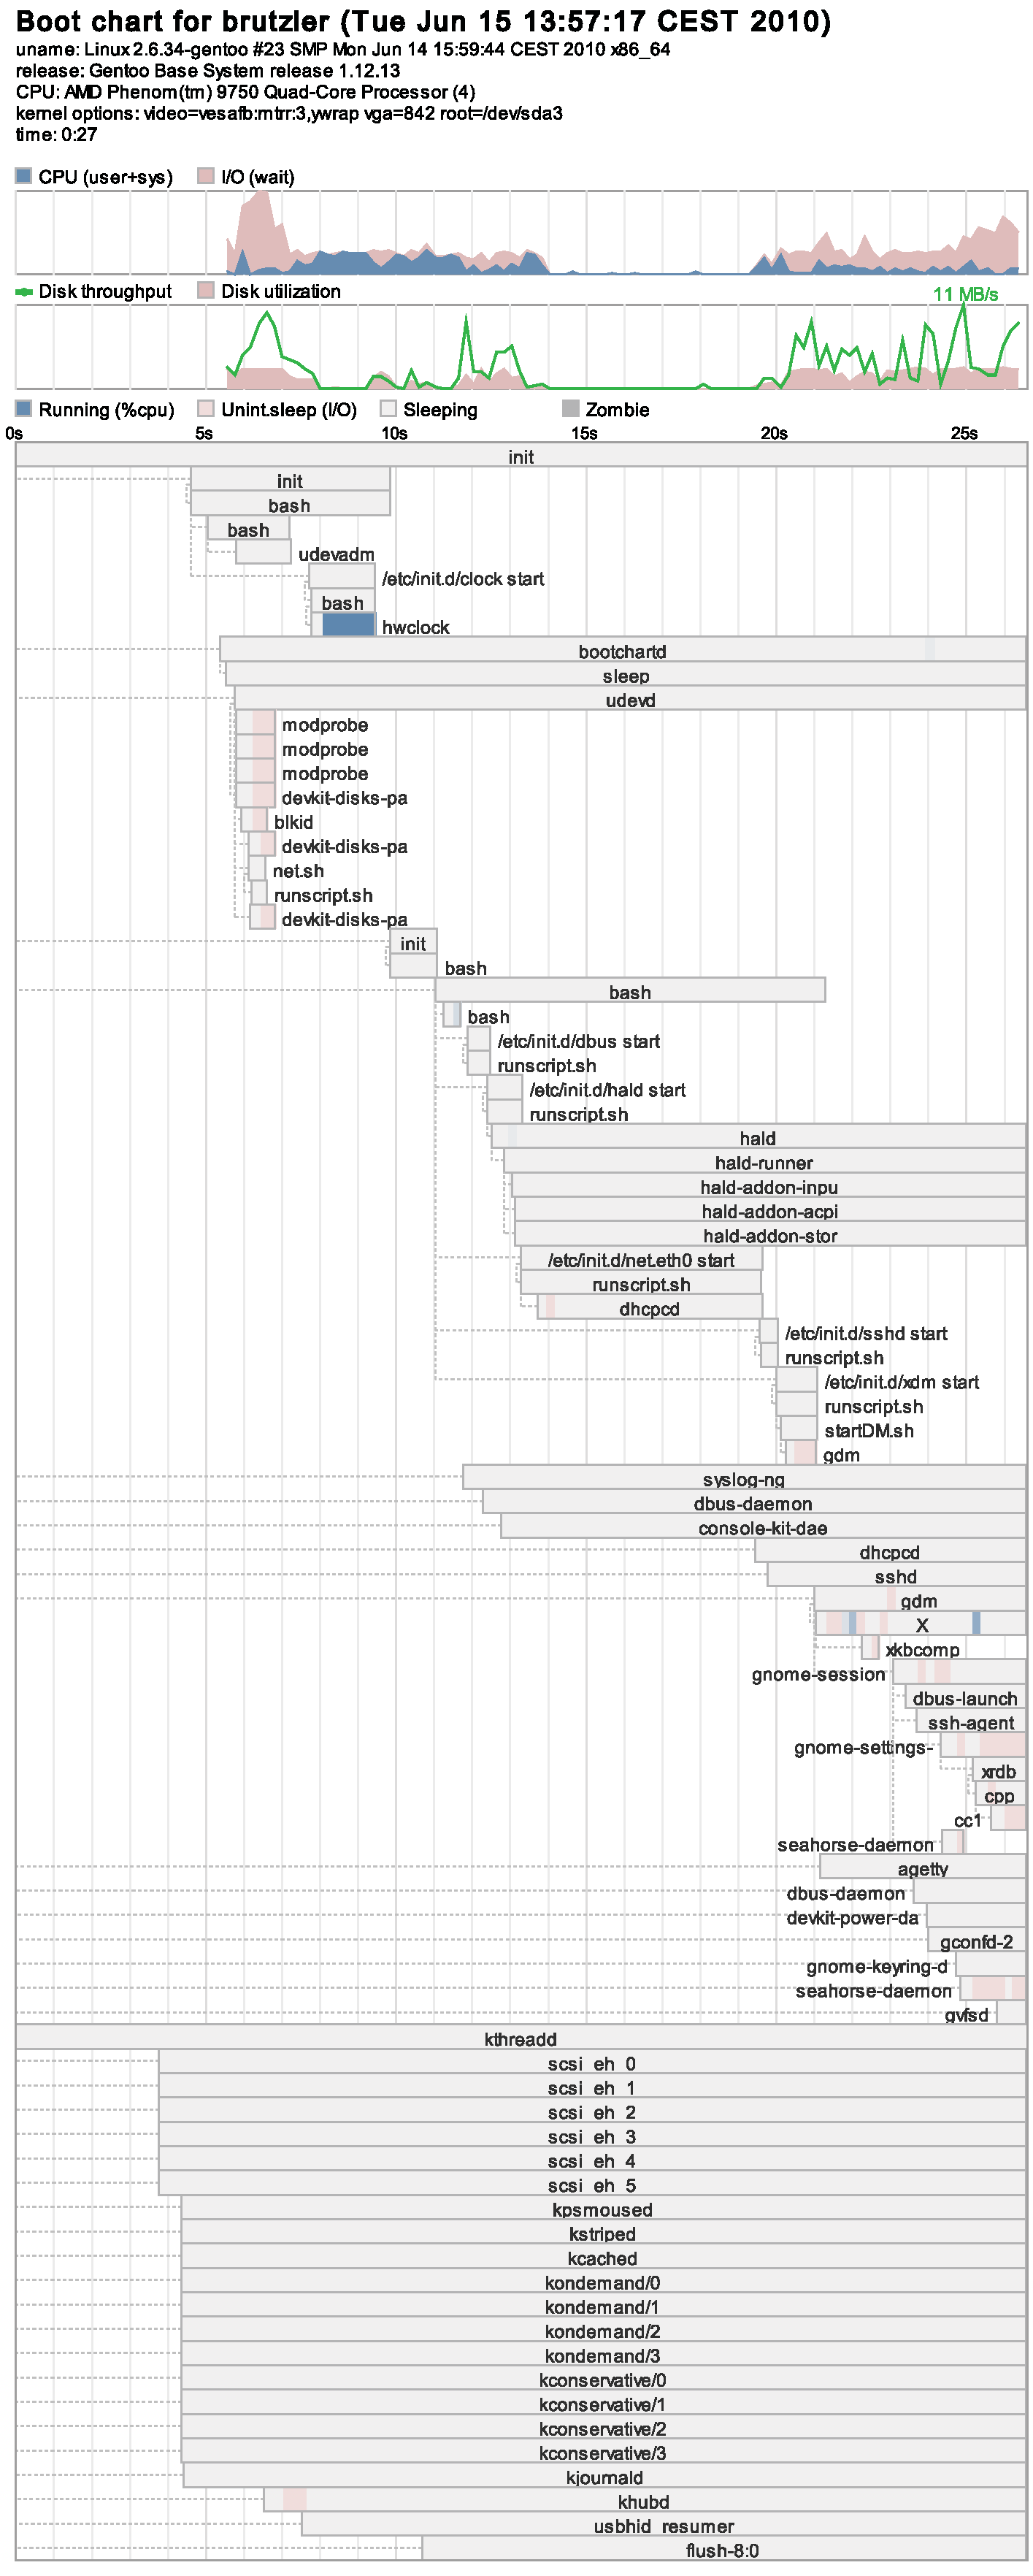
\includegraphics[scale=0.4]{figures/appendix/bootchart-hdd}
    \caption{Ausführliches Log eines HDD-Bootvorgangs}
    \label{img:bootchart-hdd}
\end{figure}

\begin{figure}[H]\centering
	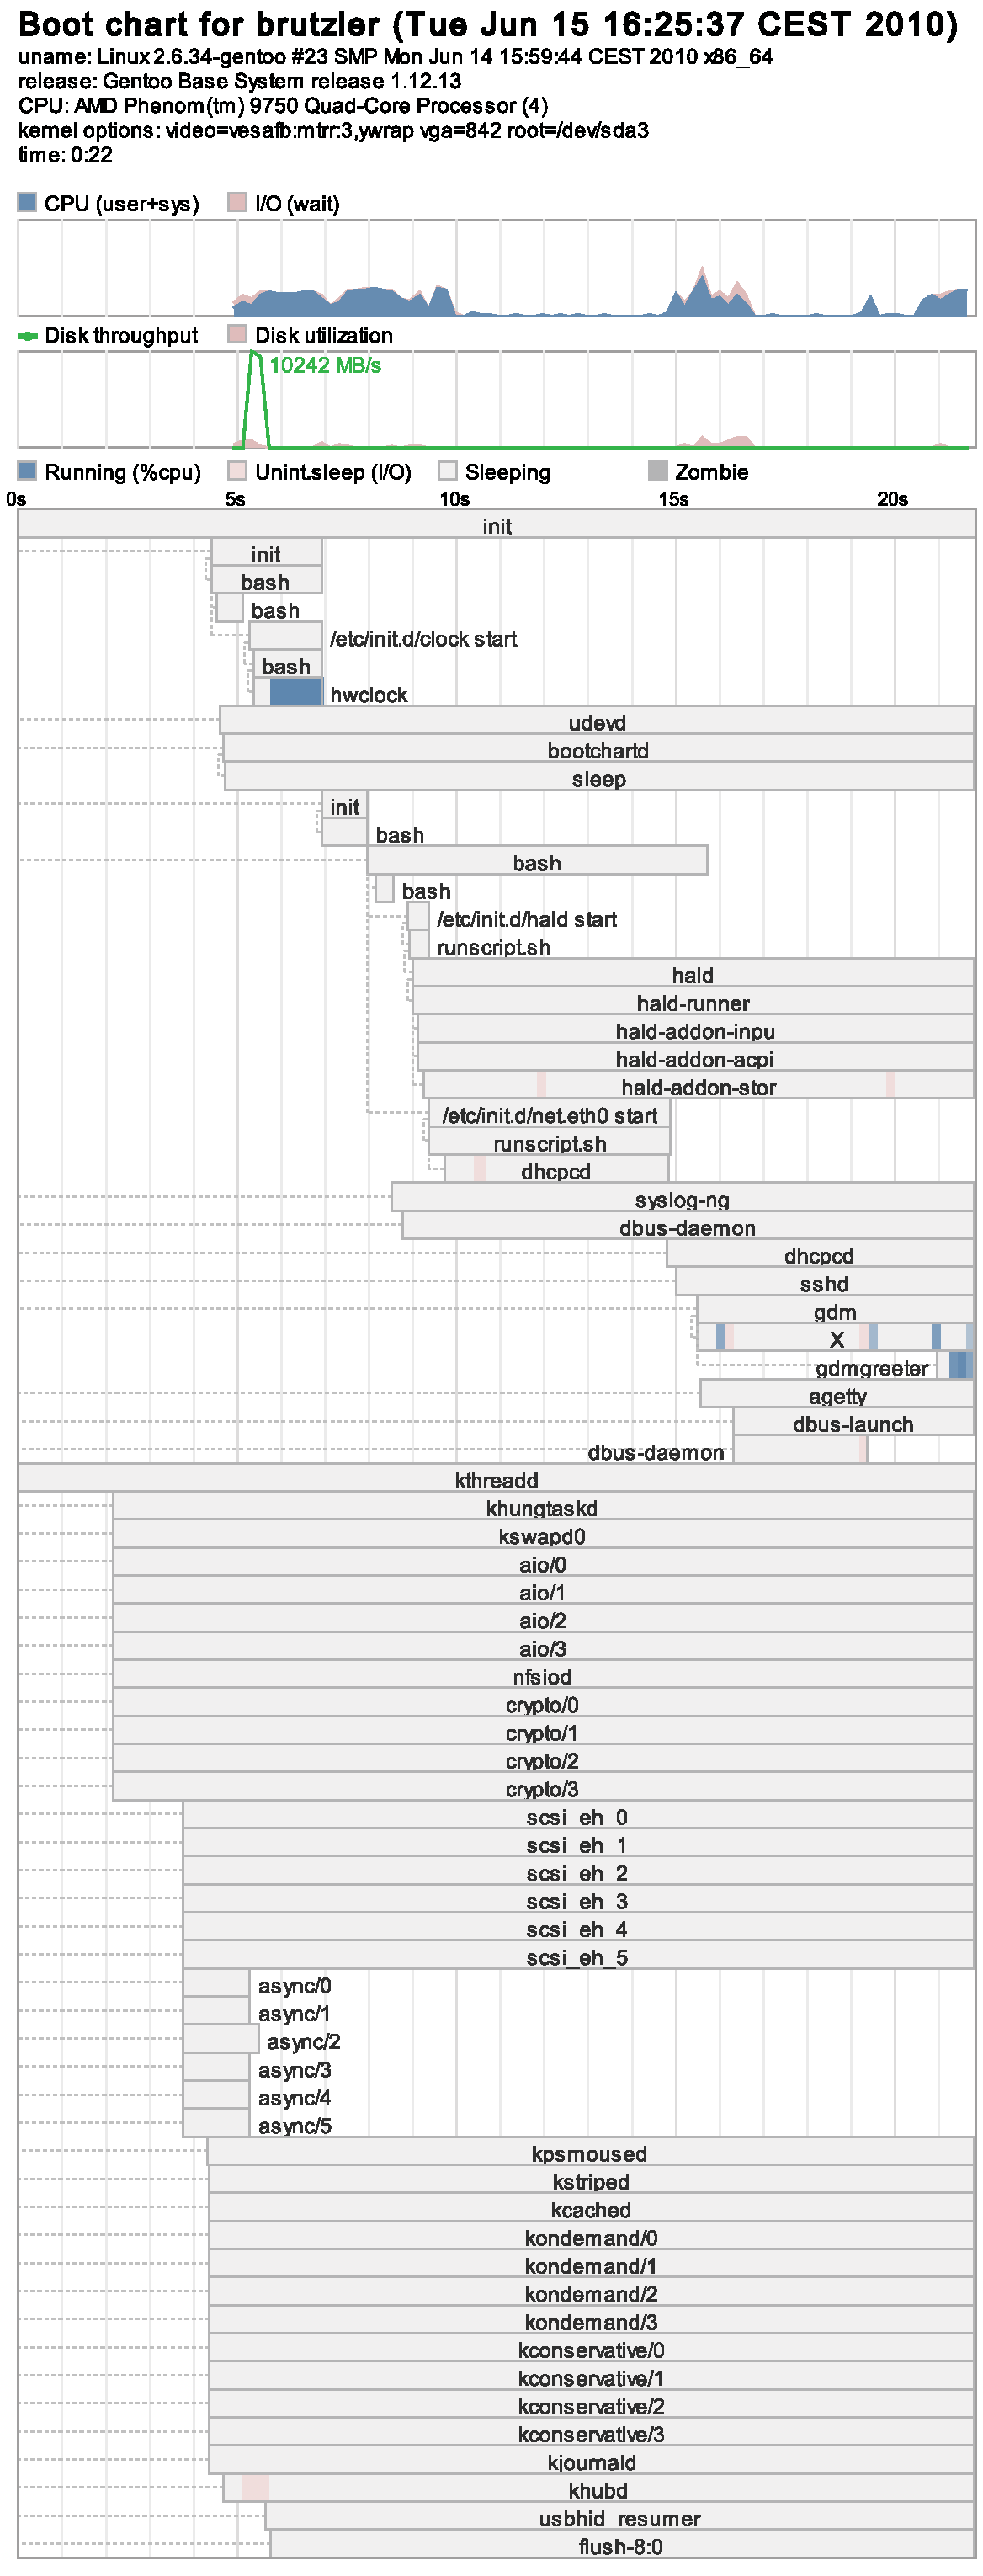
\includegraphics[scale=0.4]{figures/appendix/bootchart-ssd}
    \caption{Ausführliches Log eines SSD-Bootvorgangs mit OCZ SSD}
    \label{img:bootchart-ssd}
\end{figure}

\begin{figure}[H]\centering
	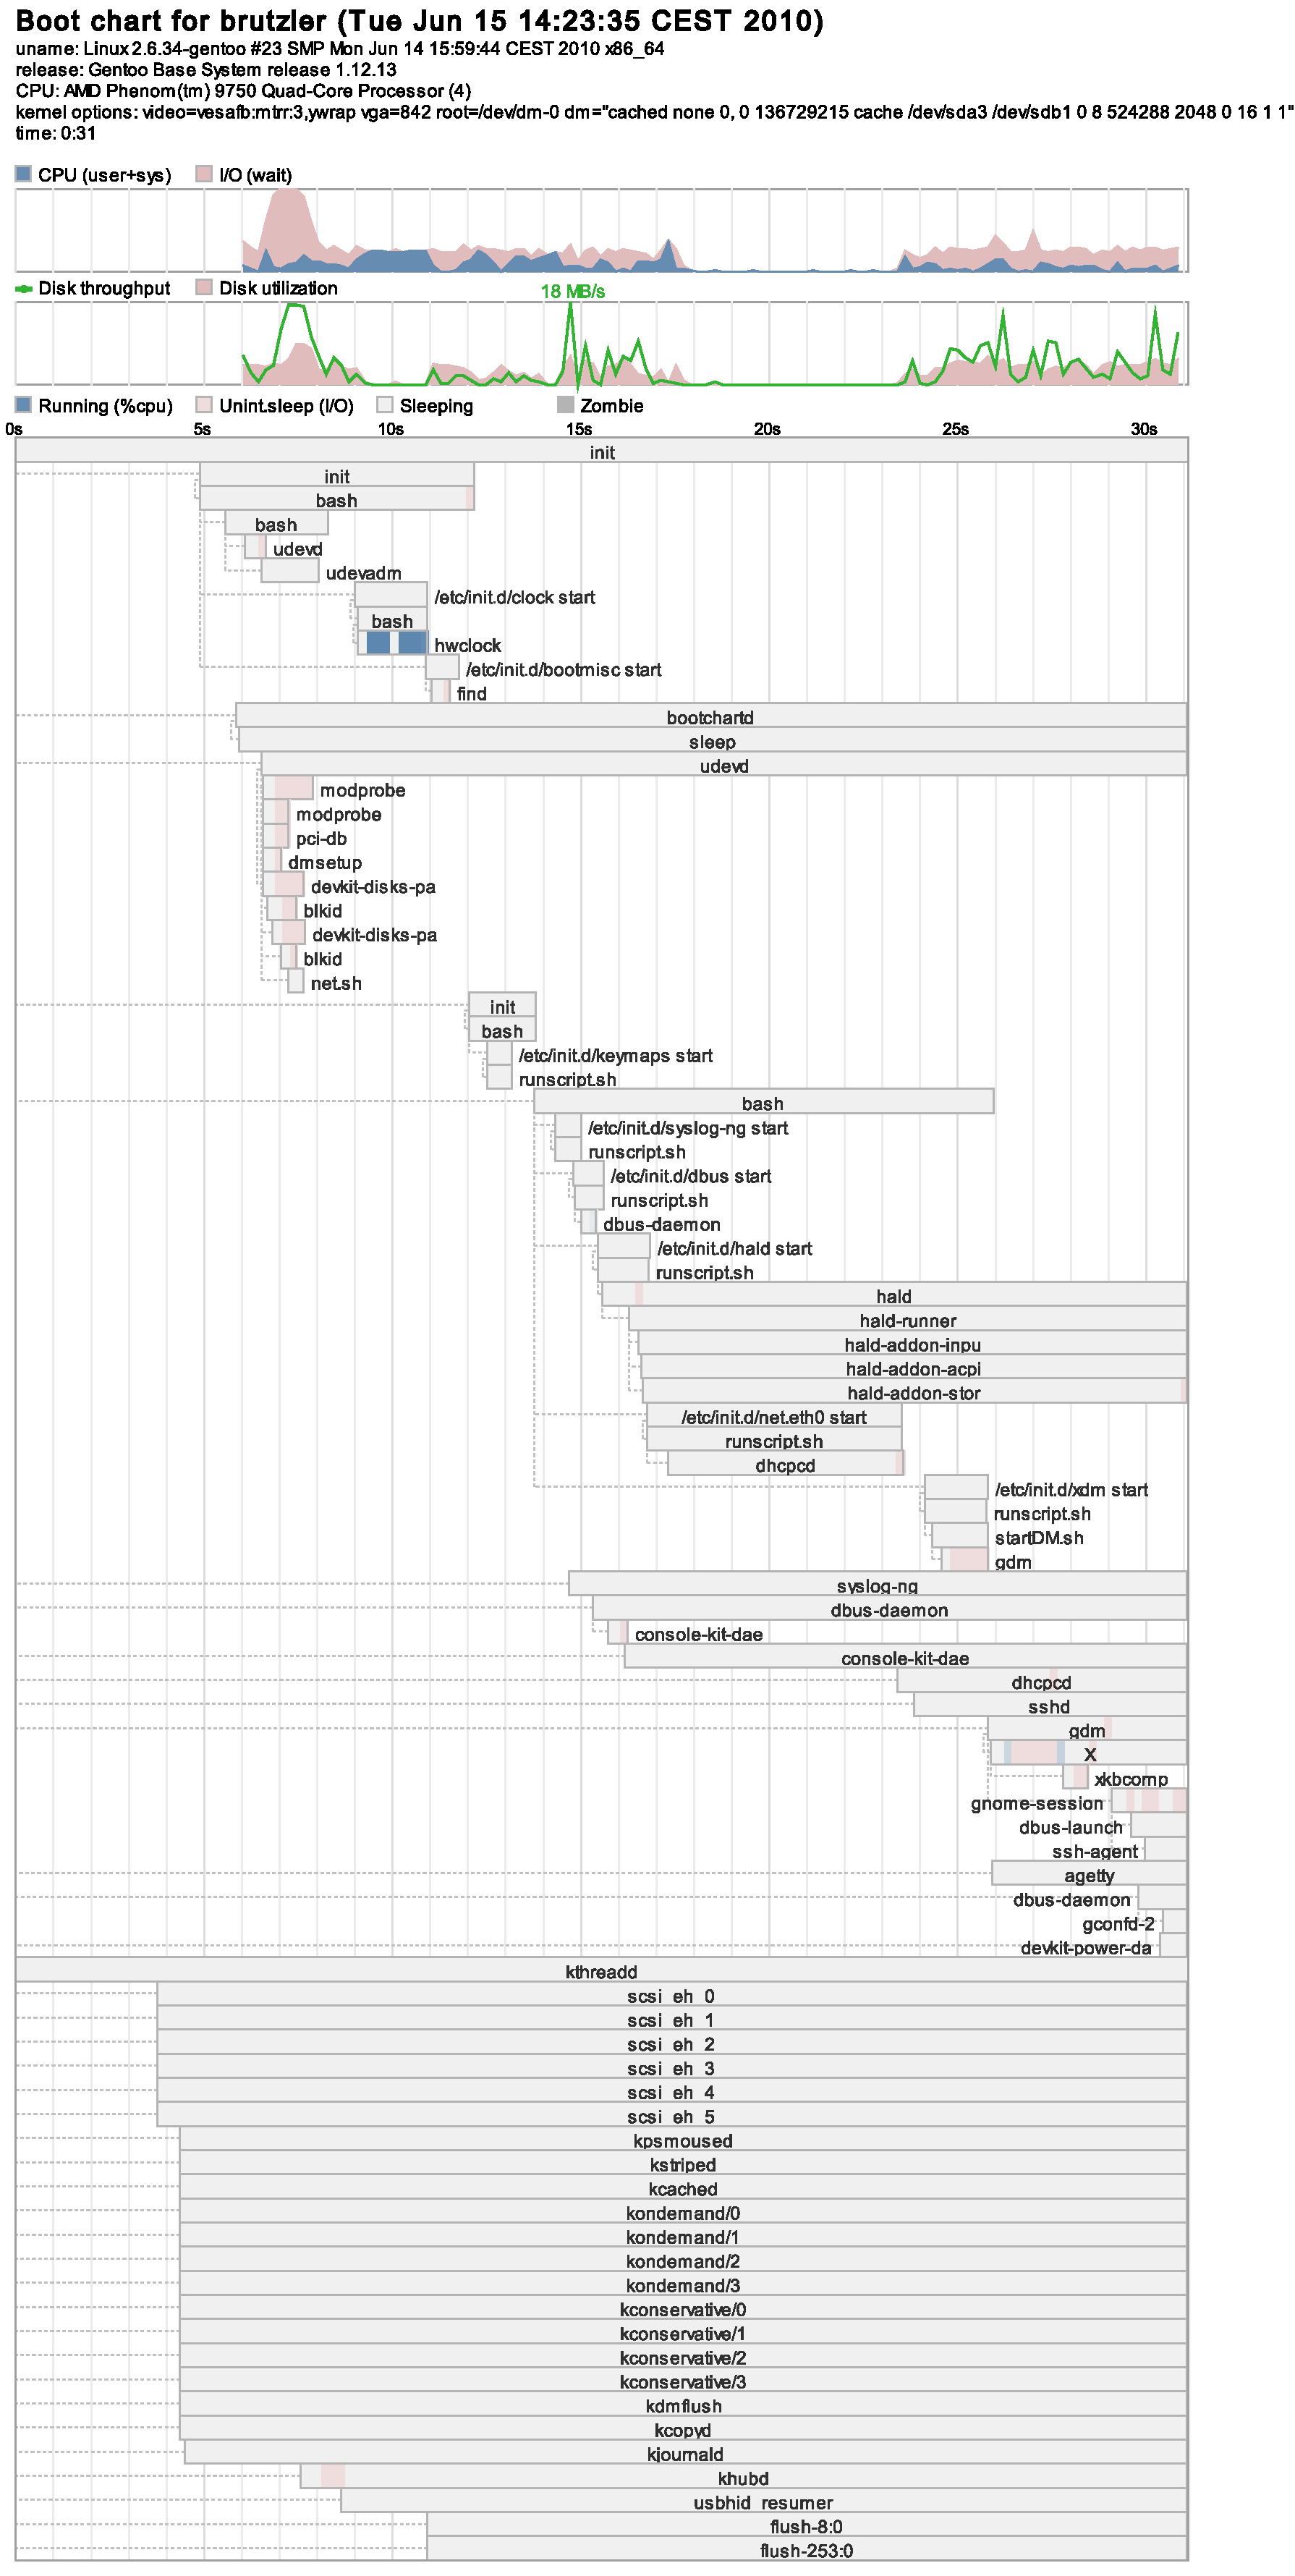
\includegraphics[scale=0.4]{figures/appendix/bootchart-cache1}
    \caption{Ausführliches Log des ersten Cache-Bootvorgangs mit OCZ SSD}
    \label{img:bootchart-cache1}
\end{figure}

\begin{figure}[H]\centering
	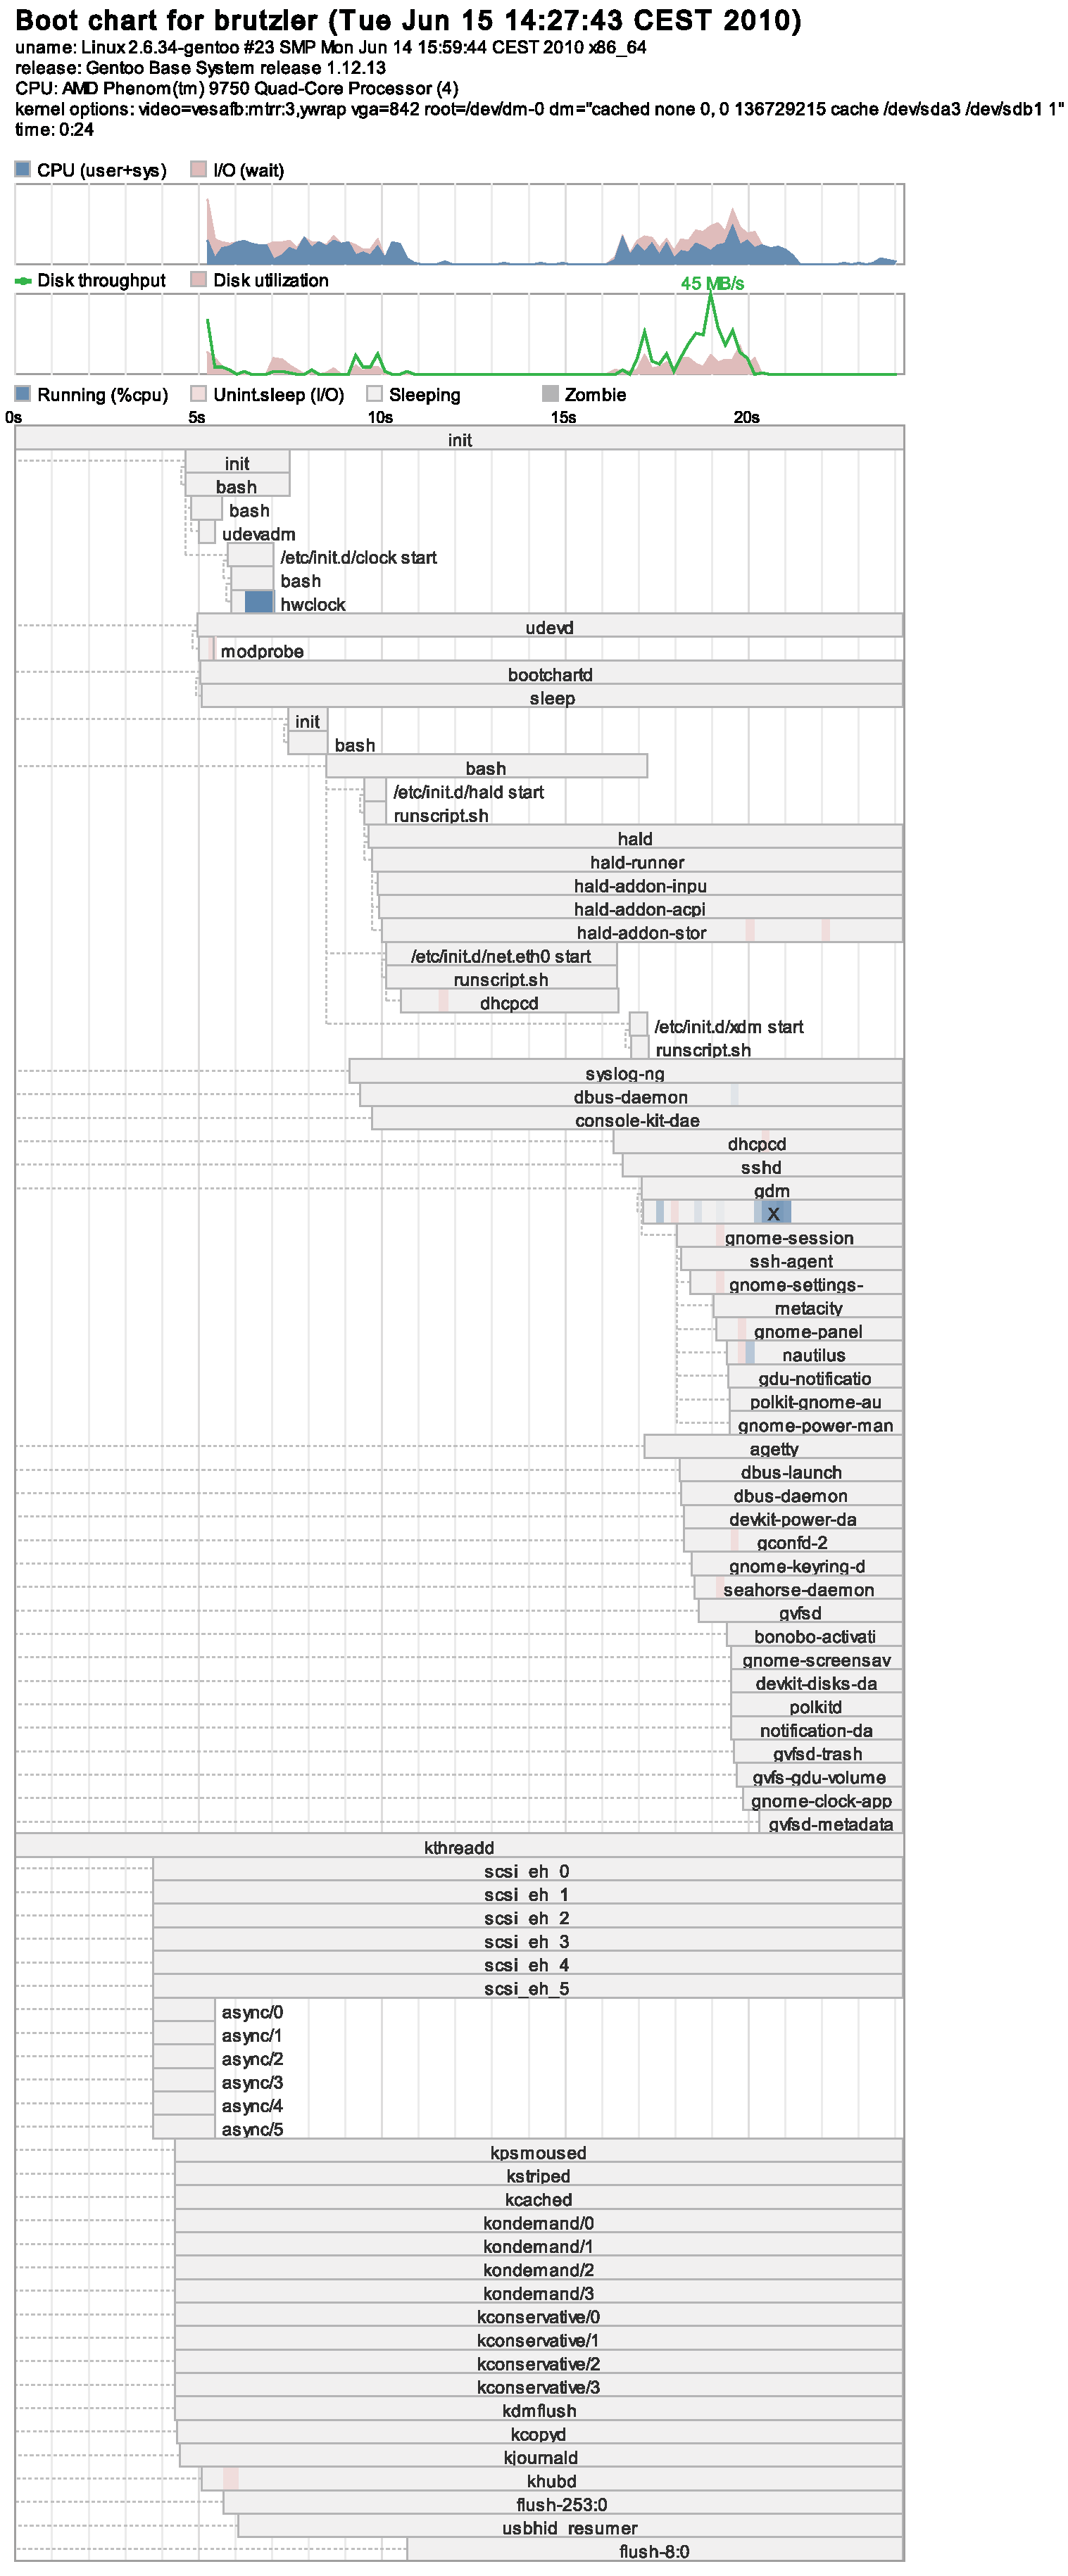
\includegraphics[scale=0.4]{figures/appendix/bootchart-cache2}
    \caption{Ausführliches Log des zweiten Cache-Bootvorgangs mit OCZ SSD}
    \label{img:bootchart-cache2}
\end{figure}

\begin{figure}[H]\centering
	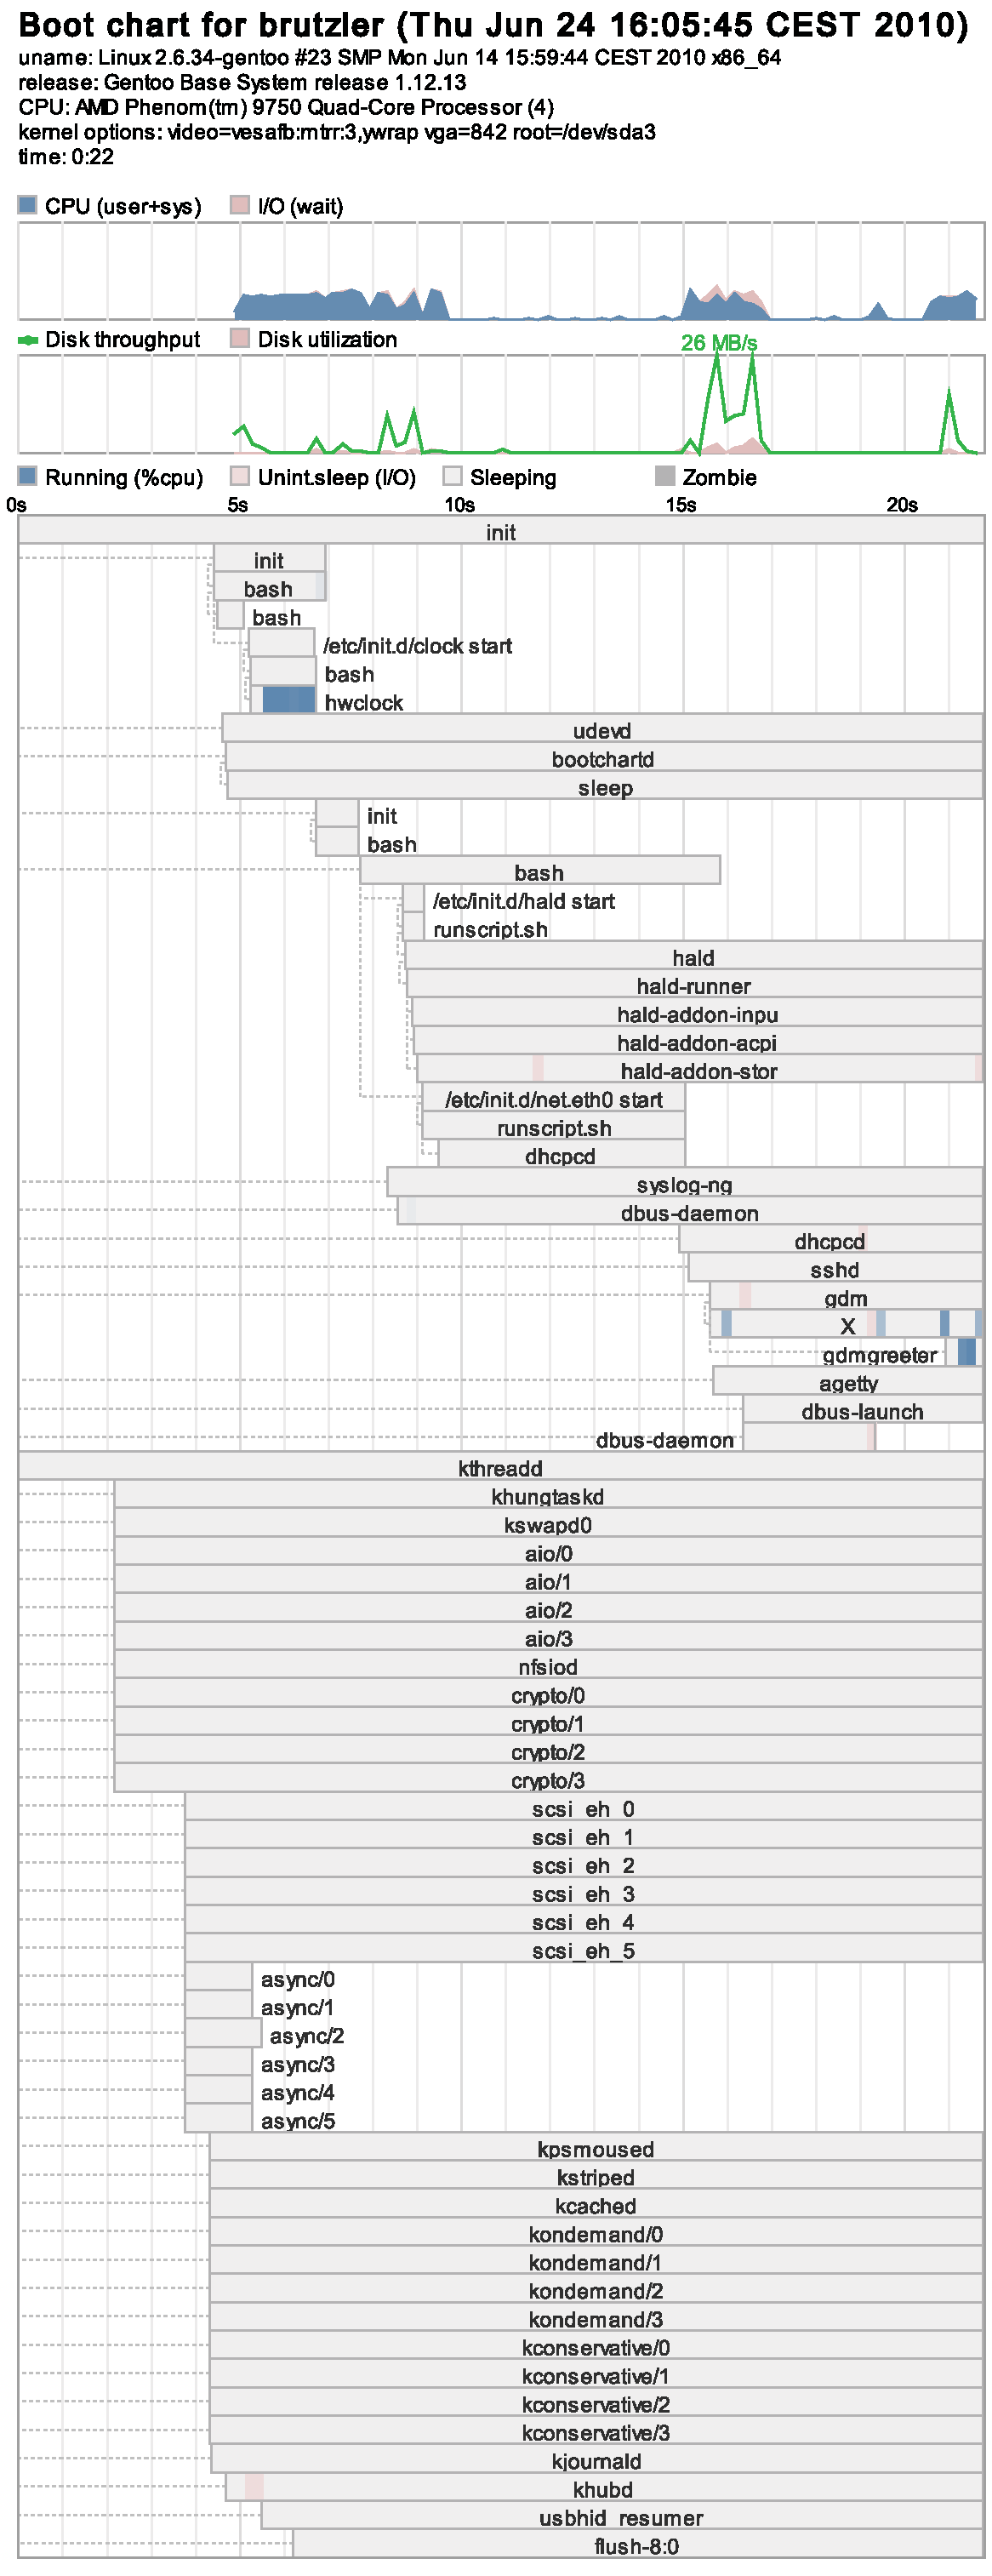
\includegraphics[scale=0.4]{figures/appendix/bootchart-ssd_intel}
    \caption{Ausführliches Log eines SSD-Bootvorgangs mit Intel SSD}
    \label{img:bootchart-ssd:intel}
\end{figure}

\begin{figure}[H]\centering
	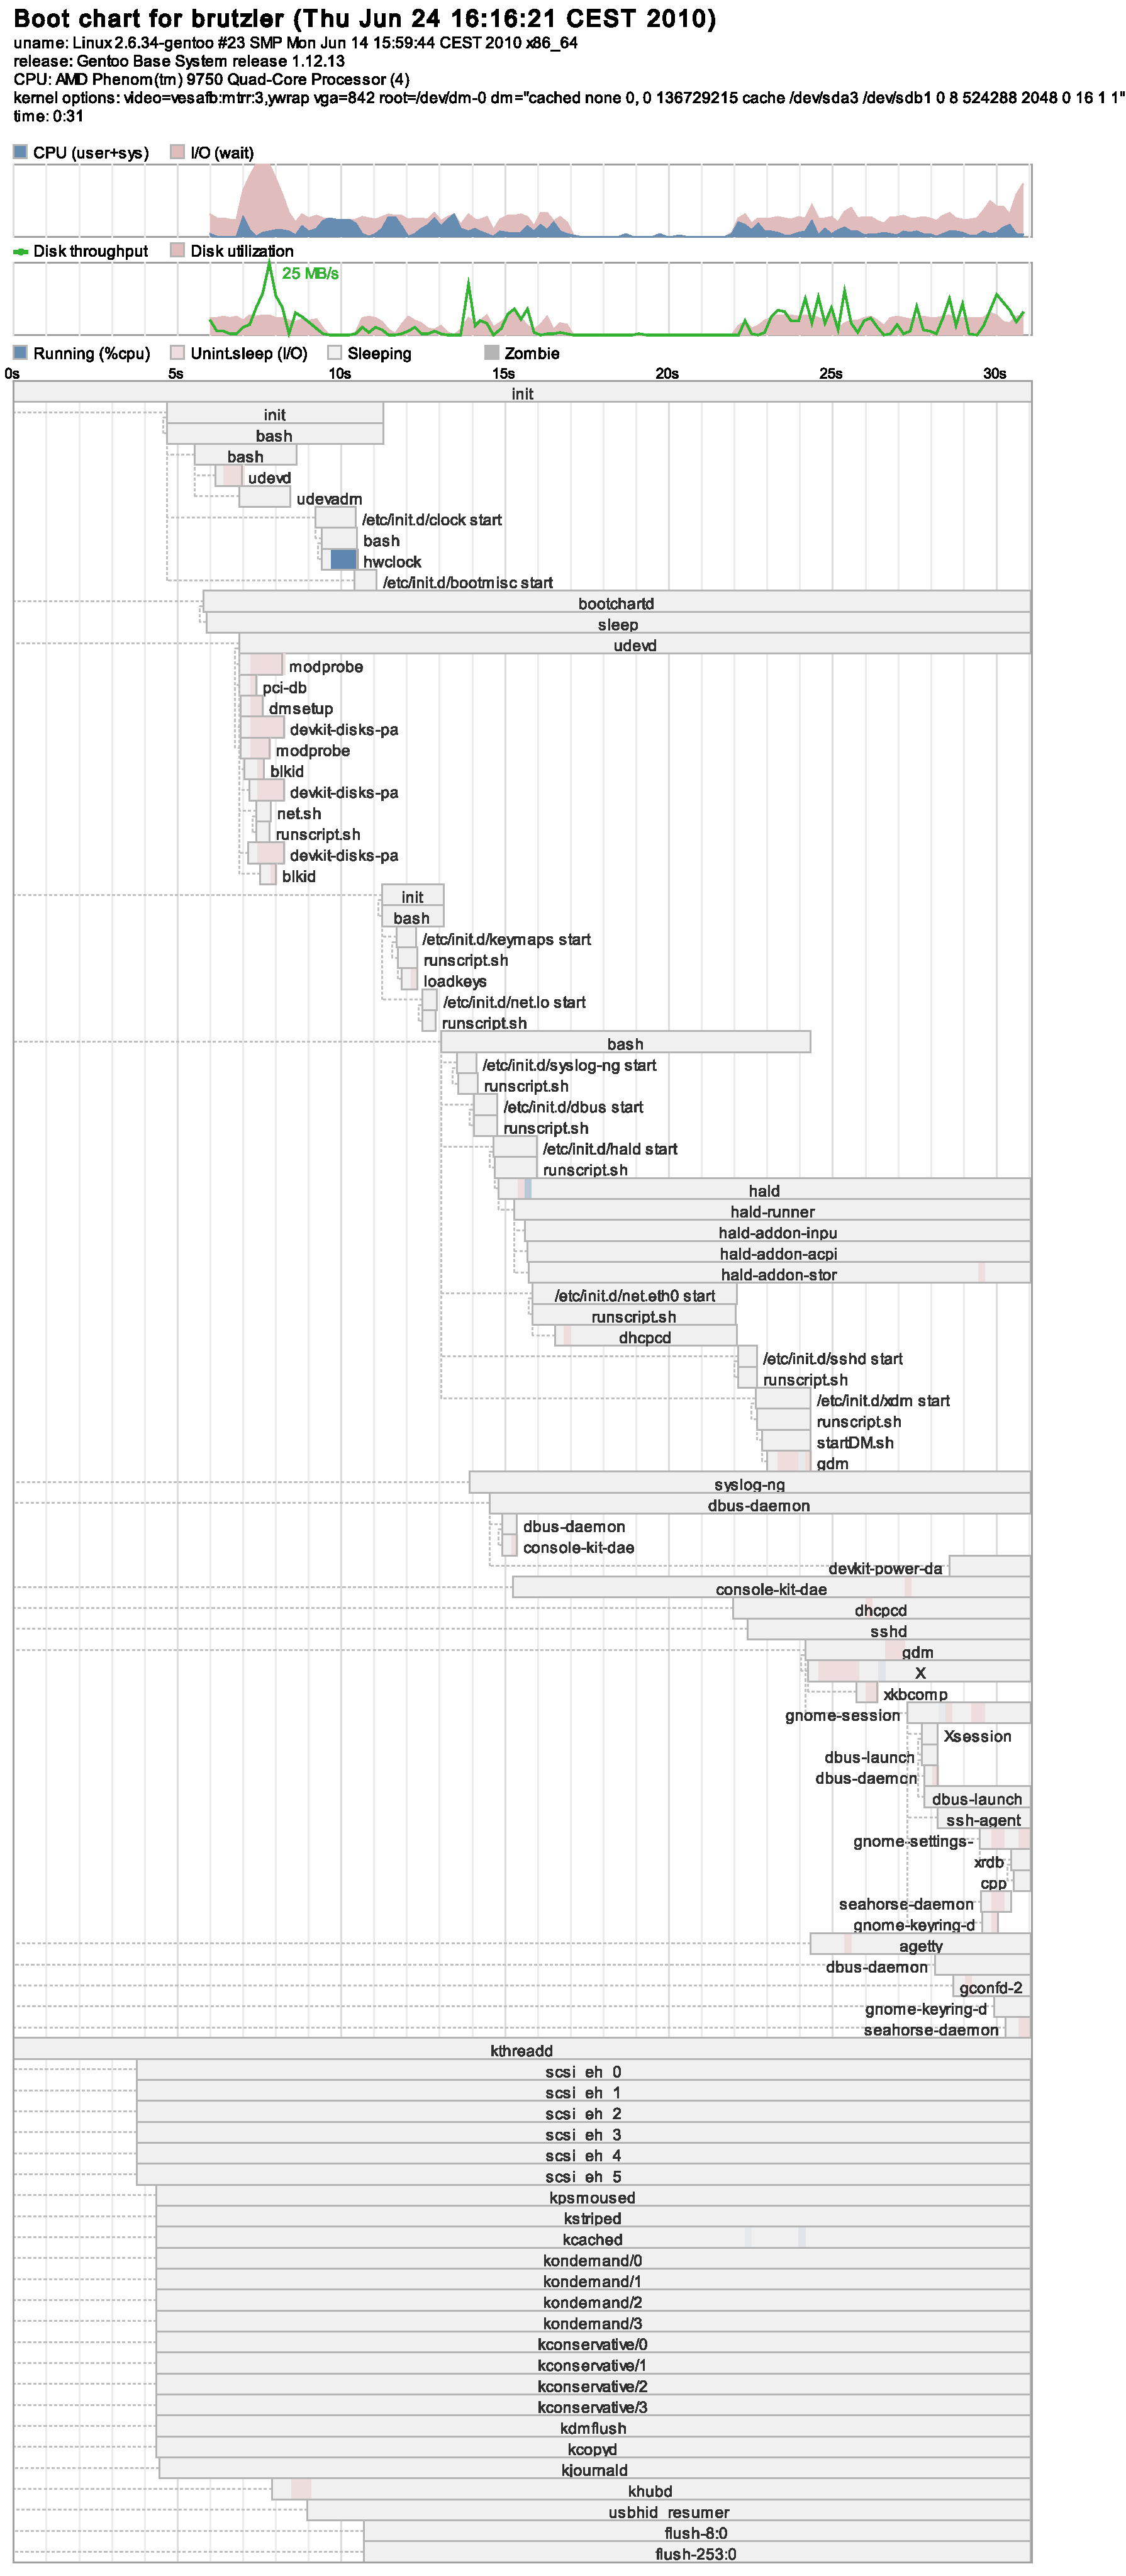
\includegraphics[scale=0.35]{figures/appendix/bootchart-cache1_intel}
    \caption{Ausführliches Log des ersten Cache-Bootvorgangs mit Intel SSD}
    \label{img:bootchart-cache1:intel}
\end{figure}

\begin{figure}[H]\centering
	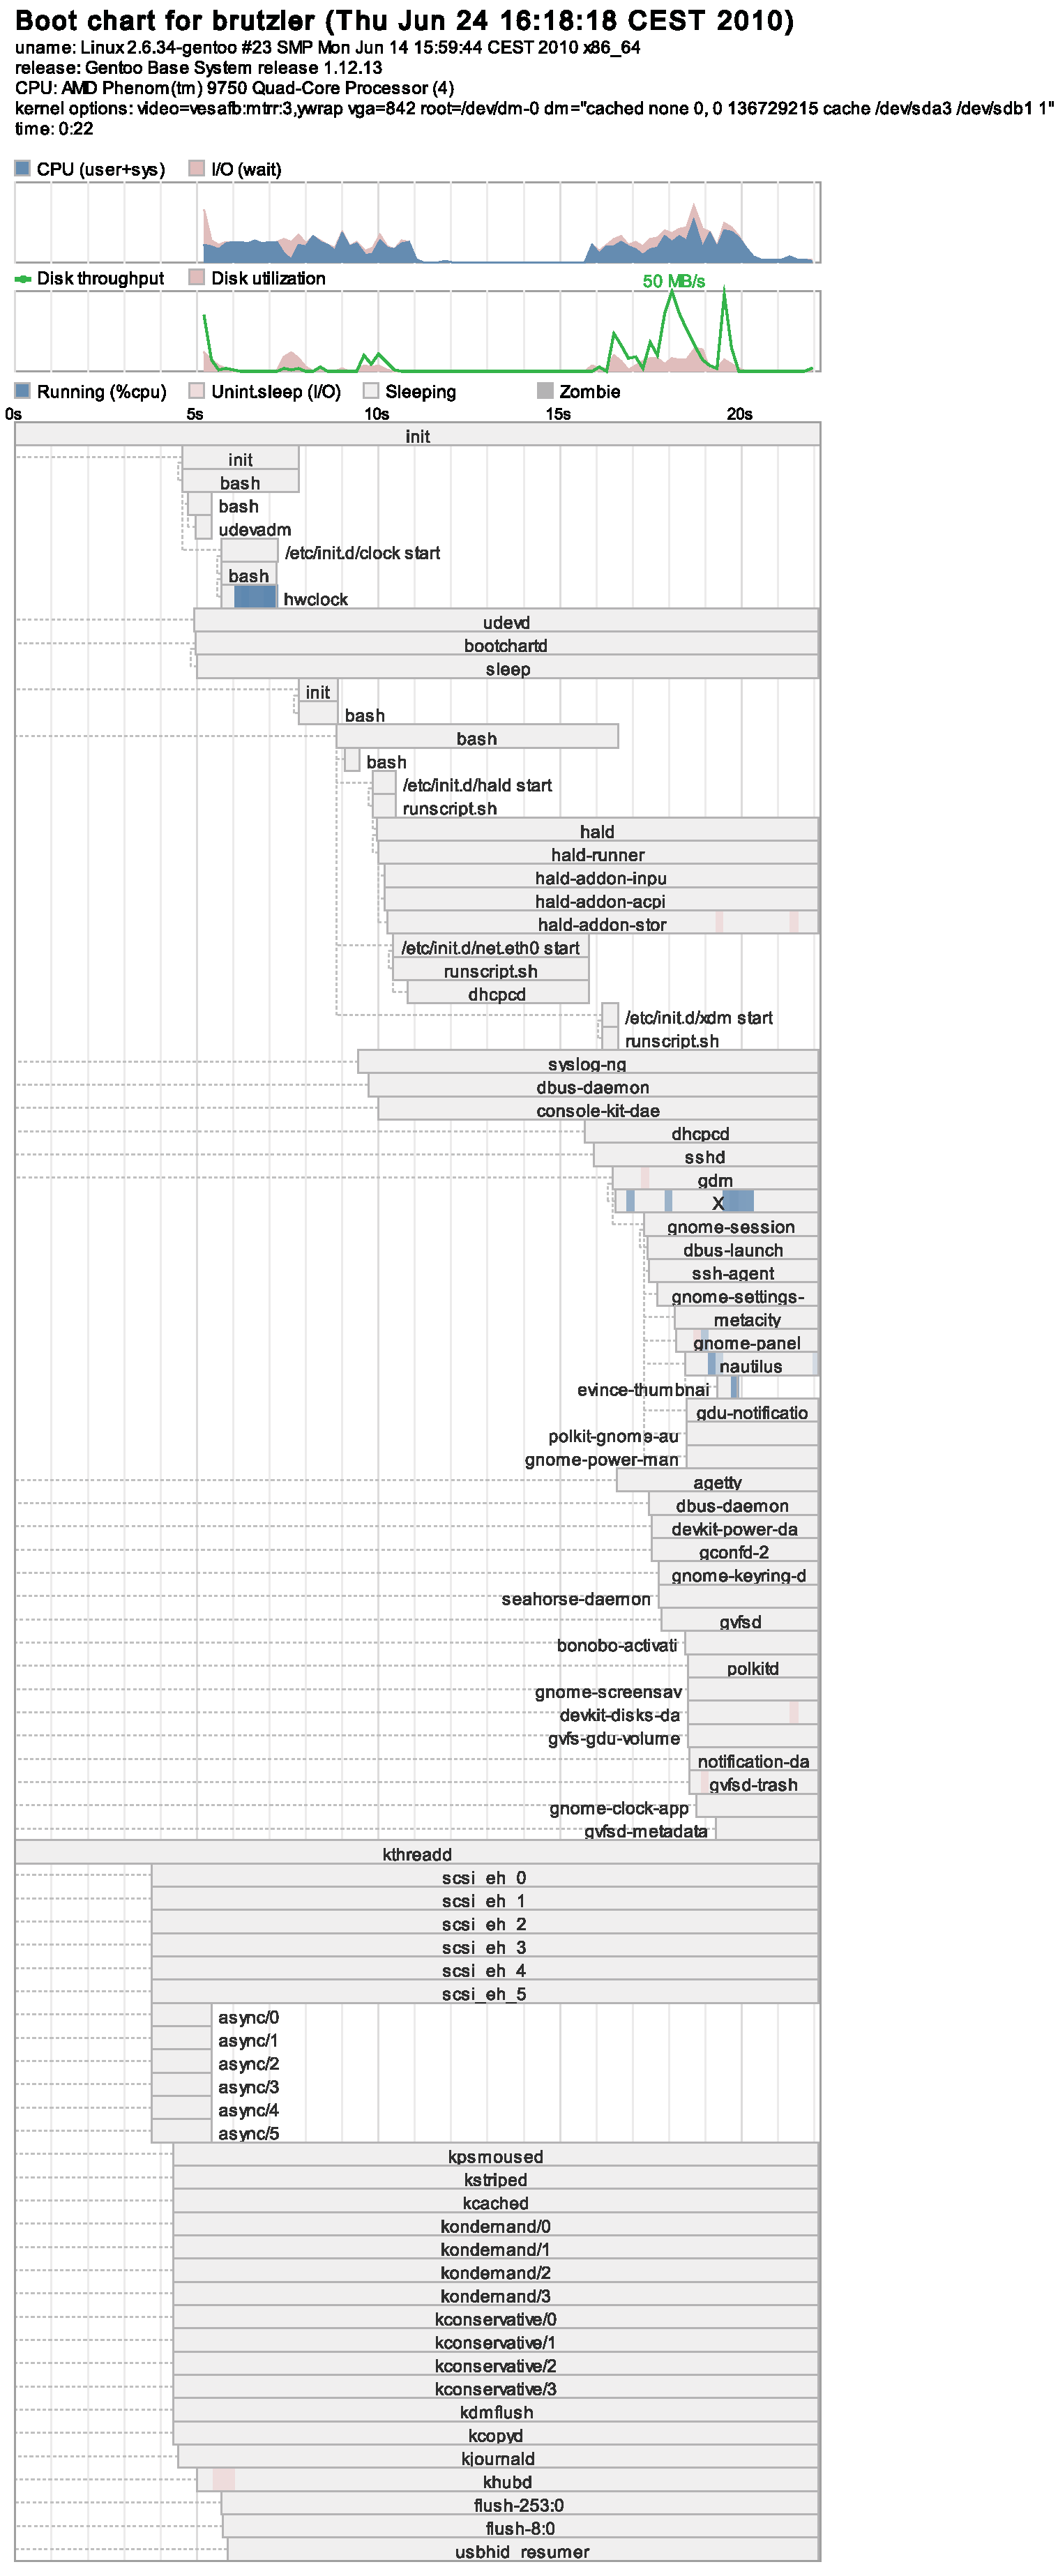
\includegraphics[scale=0.4]{figures/appendix/bootchart-cache2_intel}
    \caption{Ausführliches Log des zweiten Cache-Bootvorgangs mit Intel SSD}
    \label{img:bootchart-cache2:intel}
\end{figure}

\section*{Listings}
\sectionmark{Listings}
\addcontentsline{toc}{section}{Listings}

\subsection*{Linux Kernel}

\lstinputlisting[frame=trbl,caption=Kernelinterne Respräsentation eines \ac{BIO} (Quelle: \cite{src:linux}), label=listing:bio]{listings/struct_bio.source}

\newpage

\subsection*{dm-cache Modul}

\begin{minipage}{\textwidth}
\lstinputlisting[frame=trbl,caption=Datenstruktur für Cachemetainformationen (Quelle: \cite{src:dm-cache}), label=listing:cache1:meta]{listings/struct_cache_c1.source}

\lstinputlisting[frame=trbl,caption=Datenstruktur für Cacheblock-Metainformationen (Quelle: \cite{src:dm-cache}), label=listing:cache1:block]{listings/struct_cacheblock1.source}

\lstinputlisting[frame=trbl,caption=Datenstruktur für Auftragsliste des dm-cache (Quelle: \cite{src:dm-cache}), label=listing:cache1:job]{listings/struct_kcached_job.source}
\end{minipage}

\newpage

\subsection*{Erweitertes und optimiertes dm-cache Modul}

\lstinputlisting[frame=trbl,caption=Erweiterte Datenstruktur für Cache-Metainformationen, label=listing:cache2:meta]{listings/struct_cache_c2.source}
       \cleardoublepage{}

% References %%%%%%%%%%%%%%%%%%%%%%%%%%%%%%%%%%%%%%%%%%%%%%%%%%%%%%%%%%%%%%%%%
%%%%%%%%%%%%%%%%%%%%%%%%%%%%%%%%%%%%%%%%%%%%%%%%%%%%%%%%%%%%%%%%%%%%%%%%%%%%%%
\phantomsection
\addcontentsline{toc}{chapter}{Literaturverzeichnis}
\chaptermark{Literaturverzeichnis}
\sectionmark{Literaturverzeichnis}
\printbibliography                \clearpage{}
\chaptermark{} \sectionmark{}     \cleardoublepage{}

%% Temporarily enlarge this page to push
%% down the bottom margin
\pagestyle{empty}
\mbox{}\clearpage{}
\vspace*{5mm}
\begin{center}
\begin{minipage}{.8\textwidth}
\titleFont \large
\Author \newline
\titleFontBold \Large
\Title \newline
\titleFont \normalsize

\setlength{\parskip}{1em}

Diese Arbeit beschäftigt sich mit der Frage, ob es möglich und sinnvoll ist ein
Solid State Drive (SSD) als Cache für eine herkömmliche Magnetscheiben-basierte
Festplatte zu nutzen.

In aktuellen Rechnersystemen stellt häufig der Massenspeicher in Form einer
Festplatte den Flaschenhals des Systems dar. Dies ist darauf zurückzuführen,
dass Festplatten auf Grund ihres mechanischen Aufbaus eine Zugriffszeit haben,
die um mehrere Größenordnungen schlechter ist als die der nächsten Stufe in der
Speicherhierarchie -- dem Arbeitsspeicher. Um dieses Problem zu beseitigen,
wurde in den letzten Jahren halbleiterbasierter Massenspeicher als Ersatz für
Festplatten eingeführt, der dieses Defizit nicht besitzt. Diese Laufwerke werden
unter der Bezeichnung SSD vermarktet. SSDs haben jedoch den Nachteil, dass die
Kosten pro Byte wesentlich über denen von Festplatten liegen. Darum ist mit
einer vollständigen Substitution von Festplatten durch SSDs in den kommenden
Jahren kaum zu rechnen.

Die momentane Situation, die daraus resultiert, ist die, dass Anwender häufig
genutzte Daten auf einer meist kleinen SSD speichern und die restlichen Daten
auf einer langsameren Festplatte. Dieses Vorgehen ist für den Nutzer jedoch sehr
umständlich. Deshalb wird in dieser Arbeit die Nutzung von SSDs als
transparenter Cache für Festplatten vorgeschlagen. Dadurch würde nur ein
geringes Eingreifen des Nutzers erforderlich sein und es ihm trotzdem
ermöglicht, die Vorteile von SSDs zu nutzen.

Es werden im Verlauf dieser Arbeit dafür zunächst die technischen Grundlagen von
Festplatten und SSDs dargestellt und andere Arbeiten betrachtet, die ein
ähnliches Konzept verfolgen bzw. für die praktische Realisierung des Cache von
Bedeutung sind. Auf Grundlage dieser technischen und theoretischen
Rahmenbedingungen wird eine konkrete Problem- und Aufgabenstellung formuliert.
Basierend auf dieser wird eine Architektur für einen blockbasierten Cache
vorgeschlagen, deren konkrete Implementierung ebenfalls in dieser Arbeit
beispielhaft dargestellt wird. Mit Hilfe dieser Beispielimplementierung wurden
für diese Arbeit Simulationen und Messungen durchgeführt. Sie ermöglichen es die
Frage zu beantworten, ob es sinnvoll ist, eine SSD als Cache zu nutzen. Somit
wird abschließend diese Fragestellung anhand der gewonnenen Messergebnisse unter
den Gesichtspunkten der Leistungssteigerung und des zusätzlichen
Ressourcenverbrauchs durch den Cache diskutiert.

\end{minipage}
\end{center}


\end{document}
